% Options for packages loaded elsewhere
\PassOptionsToPackage{unicode}{hyperref}
\PassOptionsToPackage{hyphens}{url}
%
\documentclass[
]{book}
\usepackage{amsmath,amssymb}
\usepackage{lmodern}
\usepackage{iftex}
\ifPDFTeX
  \usepackage[T1]{fontenc}
  \usepackage[utf8]{inputenc}
  \usepackage{textcomp} % provide euro and other symbols
\else % if luatex or xetex
  \usepackage{unicode-math}
  \defaultfontfeatures{Scale=MatchLowercase}
  \defaultfontfeatures[\rmfamily]{Ligatures=TeX,Scale=1}
\fi
% Use upquote if available, for straight quotes in verbatim environments
\IfFileExists{upquote.sty}{\usepackage{upquote}}{}
\IfFileExists{microtype.sty}{% use microtype if available
  \usepackage[]{microtype}
  \UseMicrotypeSet[protrusion]{basicmath} % disable protrusion for tt fonts
}{}
\makeatletter
\@ifundefined{KOMAClassName}{% if non-KOMA class
  \IfFileExists{parskip.sty}{%
    \usepackage{parskip}
  }{% else
    \setlength{\parindent}{0pt}
    \setlength{\parskip}{6pt plus 2pt minus 1pt}}
}{% if KOMA class
  \KOMAoptions{parskip=half}}
\makeatother
\usepackage{xcolor}
\IfFileExists{xurl.sty}{\usepackage{xurl}}{} % add URL line breaks if available
\IfFileExists{bookmark.sty}{\usepackage{bookmark}}{\usepackage{hyperref}}
\hypersetup{
  pdftitle={Diagnóstico nacional de manejo territorial de recetarios oficiales, informes y medicamentos monopolio del Estado},
  pdfauthor={Proyecto de Inversión Mision PRI - 1901 Fondo Nacional de Estupefacientes},
  hidelinks,
  pdfcreator={LaTeX via pandoc}}
\urlstyle{same} % disable monospaced font for URLs
\usepackage{longtable,booktabs,array}
\usepackage{calc} % for calculating minipage widths
% Correct order of tables after \paragraph or \subparagraph
\usepackage{etoolbox}
\makeatletter
\patchcmd\longtable{\par}{\if@noskipsec\mbox{}\fi\par}{}{}
\makeatother
% Allow footnotes in longtable head/foot
\IfFileExists{footnotehyper.sty}{\usepackage{footnotehyper}}{\usepackage{footnote}}
\makesavenoteenv{longtable}
\setlength{\emergencystretch}{3em} % prevent overfull lines
\providecommand{\tightlist}{%
  \setlength{\itemsep}{0pt}\setlength{\parskip}{0pt}}
\setcounter{secnumdepth}{5}
\newlength{\cslhangindent}
\setlength{\cslhangindent}{1.5em}
\newlength{\csllabelwidth}
\setlength{\csllabelwidth}{3em}
\newlength{\cslentryspacingunit} % times entry-spacing
\setlength{\cslentryspacingunit}{\parskip}
\newenvironment{CSLReferences}[2] % #1 hanging-ident, #2 entry spacing
 {% don't indent paragraphs
  \setlength{\parindent}{0pt}
  % turn on hanging indent if param 1 is 1
  \ifodd #1
  \let\oldpar\par
  \def\par{\hangindent=\cslhangindent\oldpar}
  \fi
  % set entry spacing
  \setlength{\parskip}{#2\cslentryspacingunit}
 }%
 {}
\usepackage{calc}
\newcommand{\CSLBlock}[1]{#1\hfill\break}
\newcommand{\CSLLeftMargin}[1]{\parbox[t]{\csllabelwidth}{#1}}
\newcommand{\CSLRightInline}[1]{\parbox[t]{\linewidth - \csllabelwidth}{#1}\break}
\newcommand{\CSLIndent}[1]{\hspace{\cslhangindent}#1}
% Márgenes de páginas
\usepackage[
top=2.54cm, 			% Top margin
bottom=2.54cm, 			% Bottom margin
left=3.6cm, 			% Left margin
right=2.54cm,    		% Right margin
headheight=17pt, 		% as per the warning by fancyhdr
includehead,includefoot,
heightrounded, 			% to avoid spurious underfull messages
%showframe, 			% Uncomment to show how the type block is set on the page
]{geometry} 

% Requerido para incluir figuras
\usepackage{graphicx} 

\usepackage{tikz} 
\usetikzlibrary{plotmarks} % Paquete de plotmarks
\usetikzlibrary{shapes,arrows.meta} % Paquete para flechas

% Lenguaje Español, uso de punto en vez e coma para decimales, uso de tabla
\usepackage[spanish,es-nodecimaldot, es-tabla]{babel} 

% Personalizar listas
\usepackage{enumitem} 
\setlist{nolistsep} % Reducir espacio entre viñetas y listas numeradas

% Requerido para líneas horizontales en tablas
\usepackage{booktabs} 
%
\usepackage{multirow}
\usepackage{balance}
\usepackage{float}
\usepackage{amsmath}
\usepackage{ltablex}
\usepackage{tabularx}
\usepackage{afterpage}

% Tablas y Subtablas
\usepackage[labelfont=bf]{caption}
\usepackage[labelformat=simple, labelsep=period]{subcaption}
\renewcommand{\thesubfigure}{\Alph{subfigure}}

% Fuentes
\usepackage{avant}

%----------------------------------------------------------------------------------------
%	Colores definidos por usuario
%----------------------------------------------------------------------------------------
\usepackage{xcolor} % Required for specifying colors by name
% Definición de Color
\definecolor{ocre}{RGB}{243,102,25} 
\definecolor{cyan}{RGB}{0,137,186}
\definecolor{darkergreen}{RGB}{9,147,189}

% Se cambia por el color Pantone del año 2020 Azul Clásico
\definecolor{specialgreen}{RGB}{15,76,129} % Azul Clásico Pantone 19-4052
\definecolor{babyblue}{RGB}{181,199,211} % Baby Blue Pantone 13-4308 TCX
\definecolor{cornhusk}{RGB}{243,213,173} % Cornhusk Pantone 12-0714 TCX
\definecolor{Peach-Quartz}{RGB}{245,184,149} % Peach Quartz Pantone 13-1125 TCX

% Colores de Portada
\definecolor{bgBlue}{RGB}{42,43,53}
\definecolor{txBlue}{RGB}{66,87,158} 
\definecolor{moradoMinisterio}{RGB}{153,15,62}
\usepackage{mathptmx} 

%----------------------------------------------------------------------------------------
%	Bibliografía e índices
%----------------------------------------------------------------------------------------
%\usepackage{csquotes}	\usepackage[style=numeric,citestyle=numeric,sorting=nyt,sortcites=true,autopunct=true,
%autolang=hyphen,hyperref=true,abbreviate=false,backref=true,backend=biber,defernumbers=true]{biblatex}
%\addbibresource{bibliography.bib} % BibTeX bibliography file
%\defbibheading{bibempty}{}

% Paquete de Referenciación Natbib
\usepackage[numbers, round, sort, sectionbib]{natbib}
\renewcommand{\bibsection}{} % Para quitar la palabra bibliografía como título de esta sección o colocar otra. 
\setcitestyle{square}
\bibliographystyle{vancouver}

% Para un cálculo simple: se utiliza para espaciar correctamente los encabezados de las 
% letras índice
\usepackage{calc} 
% Requerido para hacer un índice
\usepackage{makeidx} 
% que Crear los archivos necesarios para la indexación en Latex
\makeindex 

%----------------------------------------------------------------------------------------
%	Encabezado de página
%----------------------------------------------------------------------------------------
% Requerido para la configuración de encabezado y pie de página
\usepackage{fancyhdr} 
\usepackage{lastpage}

\pagestyle{fancy}
% Configuración de fuente de texto de capítulo
\renewcommand{\chaptermark}[1]{\markboth{\sffamily\normalsize\bfseries\chaptername\ \thechapter.\ #1}{}} 
% Configuración de fuente de texto de sección
\renewcommand{\sectionmark}[1]{\markright{\sffamily\normalsize\thesection\hspace{5pt}#1}{}} 
% Configuración de fuente para el número de página en el encabezado
\fancyhf{} 
%\fancyhead[LE,RO]{\sffamily\normalsize\thepage} 
%\fancyhead[LO]{\rightmark} % Imprima el nombre de la sección más cercana en el lado izquierdo de las páginas impares
%\fancyhead[RE]{\leftmark} % Imprima el nombre del capítulo actual en el lado derecho de las páginas pares

%%\fancyhead[LE,RO]{\leftmark} 
\fancyhead[LE,RO]{} 
\fancyhead[LO,RE]{
\includegraphics[width=0.5\paperwidth]{www/logos_MinSalud_FNE.png}}

\renewcommand{\headrulewidth}{0.01pt} % De ancho de la regla debajo del encabezado
\addtolength{\headheight}{15pt} % Aumente ligeramente el espacio alrededor del encabezado
\renewcommand{\footrulewidth}{0pt} % Elimina la línea en el pie de página
\fancypagestyle{plain}{\fancyhead{}\renewcommand{\headrulewidth}{0pt}} % Estilo para cuando se especifica un estilo de página simple

%%% Configurar pie de Página
\setlength{\footskip}{40pt}
%\lfoot{\mdseries Proyecto de Inversión - Misión PRI 1901}
\cfoot{}
%\rfoot{\mdseries Página~\thepage}

\fancyfoot[LO,RE]{\mdseries Proyecto de Inversión - Misión PRI 1901}
\fancyfoot[LE,RO]{\mdseries Página~\thepage}

% Elimina el encabezado de páginas vacías impares al final de los capítulos
\makeatletter
\renewcommand{\cleardoublepage}{
	\clearpage\ifodd\c@page\else
	\hbox{}
	\vspace*{\fill}
	\thispagestyle{empty}
	\newpage
	\fi}


%% Elimina el encabezado de páginas vacías impares al final de los capítulos
%\makeatletter
%\renewcommand{\cleardoublepage}{
%	\clearpage\ifodd\c@page\else
%	\hbox{}
%	\vspace*{\fill}
%	\thispagestyle{empty}
%	\newpage
%	\fi}

%% Esto se usa para prevenir el error de flotas sobrepasados en ciclos
\usepackage[maxfloats=256]{morefloats}
\usepackage{tikz} 
\usetikzlibrary{plotmarks} 
\usetikzlibrary{shapes,arrows.meta} 

%%%%%%%%%%%%%%

\usepackage{sectsty}
\chapterfont{\bf\color{moradoMinisterio}}
\sectionfont{\bfseries \color{moradoMinisterio}}
\subsectionfont{\color{moradoMinisterio}}
\subsubsectionfont{\color{moradoMinisterio}}
\usepackage{booktabs}
\usepackage{longtable}
\usepackage{array}
\usepackage{multirow}
\usepackage{wrapfig}
\usepackage{float}
\usepackage{colortbl}
\usepackage{pdflscape}
\usepackage{tabu}
\usepackage{threeparttable}
\usepackage{threeparttablex}
\usepackage[normalem]{ulem}
\usepackage{makecell}
\usepackage{xcolor}
\ifLuaTeX
  \usepackage{selnolig}  % disable illegal ligatures
\fi

\title{Diagnóstico nacional de manejo territorial de recetarios oficiales, informes y medicamentos monopolio del Estado}
\usepackage{etoolbox}
\makeatletter
\providecommand{\subtitle}[1]{% add subtitle to \maketitle
  \apptocmd{\@title}{\par {\large #1 \par}}{}{}
}
\makeatother
\subtitle{Informe Final de Visitas Técnicas a Fondos Rotatorios de Estupefacientes}
\author{Proyecto de Inversión Mision PRI - 1901 Fondo Nacional de Estupefacientes}
\date{10 de octubre de 2021}

\begin{document}

\frontmatter

\begingroup
\thispagestyle{empty}
\begin{tikzpicture}[overlay, remember picture] %-Cambio de fondo de página
	% Crea una coordenada 12 cm por debajo del norte de la página
	\coordinate [right=11cm, below=06.5cm] (highpoint) at (current page.north west);
	\coordinate [right=11cm, below=17.5cm] (midpoint) at (current page.north west);
	\coordinate [right=11cm, below=19.0cm] (lowpoint) at (current page.north west);
	\coordinate [right=7.5cm, below=24.2cm] (finalLogo) at (current page.north west);
	% Inicia una nueva figura al nor oeste
	\node at (current page.north west)
	{
		\begin{tikzpicture}[overlay, remember picture]
			%- 
			% Imagen de Fondo
			\node[anchor=north west, inner sep=0pt] at (0,0) {
\includegraphics[width=\paperwidth]{www/Portada_1.pdf}};	
			\draw[anchor=north] (highpoint) node [fill=bgBlue, fill opacity=0.01, text opacity=1.0, inner sep=1cm,  text=txBlue]{\Huge\centering\bfseries\sffamily\parbox[c][][t]{20cm}
				{\centering Diagnóstico nacional de manejo territorial de recetarios oficiales, informes y medicamentos monopolio del Estado}};  
			\draw[anchor=north] (midpoint) node [fill=bgBlue, fill opacity=0.01, text opacity=1, inner sep=1cm, text=txBlue]{\LARGE\centering\bfseries\sffamily\parbox[c][][t]{16cm} {Proyecto de Inversión Misión PRI 1901}}; 
			\draw[anchor=north] (lowpoint) node [fill=bgBlue, fill opacity=0.01, text opacity=1, inner sep=1cm, text=txBlue]{\LARGE\centering\bfseries\sffamily\parbox[c][][t]{16cm} {10 de octubre de 2021}};
			
			\draw[anchor=north west] (finalLogo) node[inner sep=0pt] {
\includegraphics[width=0.6\paperwidth]{www/logos_MinSalud_FNE.png}};
			%%\node[inner sep=0pt] (finalLogo) {\includegraphics[width=0.3\paperwidth]{logos MinSalud_FNE.png}};
	\end{tikzpicture}};
	
\end{tikzpicture}
\vfill
\endgroup

\cleardoublepage
%----------------------------------------------------------------------------------------
%	Capítulo 0 Página de Inicio
%----------------------------------------------------------------------------------------
%\newpage
\hypertarget{TitlePage}{}
\bookmark[dest=TitlePage, level=-1, view=Fit]{Informe Final de Visitas Técnicas a Fondos Rotatorios de Estupefacientes (FRE)}
%\bookmark[dest=tocpage, level=0, named=tocpage]{title}
%\pdfbookmark[-1]{Farmacocinética poblacional en el manejo empírico de infecciones en pacientes con neoplasias hematológicas y neutropenia febril posquimioterapia}{}
%\setcounter{page}{1}
\begin{center}
	\begin{figure}
		\centering%
		
\includegraphics[width=\linewidth]{www/logos_MinSalud_FNE.png}
	\end{figure}
	\thispagestyle{empty} 
	\vspace*{0.4cm}	
	\huge{\bfseries\sffamily\textbf{
			Diagnóstico nacional de manejo territorial de recetarios oficiales, informes y medicamentos monopolio del Estado}}\\[3.7cm]
	\large{\bfseries\sffamily\textbf{
			Informe Final de Visitas Técnicas a Fondos Rotatorios de Estupefacientes (FRE)}}\\[3.7cm]	
	\Large{\bfseries\sffamily\textbf{
			Proyecto de Inversión Misión PRI 1901}}\\[3.7cm]
	\normalsize{\sffamily{
			Fondo Nacional de Estupefacientes\\
			Ministerio de Salud y Protección Social de Colombia\\
			Bogotá D.C., Colombia\\
			2021}}\\
\end{center}


\newpage
~\vfill
\thispagestyle{empty}
\noindent Copyright \copyright\ 2021 Fondo Nacional de Estupefacientes \\ % Copyright notice
\noindent \textsc{Publicado por el Fondo Nacional de Estupefacientes}\\ % Publisher
%%\noindent \textsc{Dirección de Contacto: dsparrag@unal.edu.co}\\ % URL
\noindent \textit{Primera Impresión, Agosto 2021} \\ % Printing/edition date
\medskip
\medskip
\medskip


%%%%%%%%%\maketitle
%%%%%%%%%
\cleardoublepage
%%% \pagestyle{empty}
\thispagestyle{empty}
\hypertarget{tocpage}{}
\renewcommand*\contentsname{Tabla de Contenidos}
{
\setcounter{tocdepth}{2}
\tableofcontents
}
\bookmark[dest=tocpage, level=0, named=tocpage, color=moradoMinisterio]{\contentsname} %\pdfbookmark[0]{\contentsname}{toc}

\cleardoublepage\phantomsection
\renewcommand{\listfigurename}{Lista de figuras}
\addcontentsline{toc}{chapter}{\listfigurename}
\listoffigures

%%% 
\cleardoublepage\phantomsection
\renewcommand{\listtablename}{Lista de tablas}
\addcontentsline{toc}{chapter}{\listtablename}
\listoftables

%%% 
\mainmatter
\hypertarget{prefacio}{%
\chapter*{Prefacio}\label{prefacio}}
\addcontentsline{toc}{chapter}{Prefacio}

El FNE (\emph{Fondo Nacional de Estupefacientes}) tiene como objetivo la vigilancia y control sobre la importación, la exportación, la distribución y venta de drogas, medicamentos, materias primas o precursores de control especial, a que se refiere la Ley 30 de 1986 y las demás disposiciones que expida el Ministerio de la Protección Social, así como apoyar a los programas contra la farmacodependencia que adelanta el Gobierno Nacional.

En los últimos años, la planeación de las cantidades de medicamentos monopolio del Estado (MME) para satisfacer la demanda en los entes territoriales se ha visto afectada por:

\begin{itemize}
\item
  La variabilidad en el incremento o disminución de la distribución y necesidad de MME.
\item
  La participación en las guías de tratamiento farmacológico de cada uno de estos medicamentos y que se ve afectada por las diferentes recomendaciones internacionales.
\item
  La calidad de la información de disponibilidad remitida por los FRE.
\item
  Las diferentes barreras administrativas de índole territorial que impactan en el acceso de estos medicamentos por parte de los pacientes.
\end{itemize}

Por consiguiente, el desarrollo de este proyecto se enmarca en una estrategia integral con el fin de contribuir a mejorar la calidad de la atención de los pacientes y a la salud pública del país, garantizando el acceso, disponibilidad y uso racional de los medicamentos de control especial y MME.

El proyecto tiene como producto entregable una fuente de información caracterizada y consolidada para el desarrollo del Recetario Oficial Electrónico (ROE), de tal manera que se determine el rol del FNE, FRE y las IPS para fortalecer el seguimiento a las prescripciones de medicamentos monopolio del Estado, encaminados al uso racional de estos medicamentos en todo el territorio nacional y una fuente de información caracterizada y consolidada para el desarrollo de una herramienta que permita estandarizar los procesos de proyección de compra y el seguimiento de inventarios de MME por parte de los entes territoriales, de tal manera que se mitigue el riesgo de desabastecimiento mediante la gestión de inventarios acorde a las necesidades de la población.

El trabajo territorial es una experiencia de aprendizaje recíproco y constante. Dentro de las Jornadas de inmersión territorial se observó, no solamente las condiciones actuales en la que se encuentran los FRE alrededor de la nación, sino el entusiasmo con la que los funcionarios se interesan por el bienestar y la salud pública de su región, aún cuando se presentan diferentes adversidades y vicisitudes en sus departamentos.

Agradecemos a cada referente de cada FRE y a cada funcionario de apoyo, por tan acogedor recibimiento del que hicieron partícipe al equipo territorial del Proyecto de Inversión 1901, reafirmando que parte de la belleza de Colombia es la calidez y amabilidad de sus habitantes. También queremos agradecer al FNE y a su íntegro equipo, coordinadores y apoyos territoriales, por brindarnos todos los recursos, herramientas y ser una guía para llevar a cabo el proceso de investigación.

\hypertarget{introducciuxf3n}{%
\chapter{Introducción}\label{introducciuxf3n}}

Con motivo de presentar la metodología del trabajo territorial que se adelanta en el marco del proyecto de inversión 1901 \texttt{Incremento\ de\ la\ disponibilidad\ de\ medicamentos\ Monopolio\ del\ Estado\ para\ los\ pacientes\ en\ Colombia\ Nacional\ Código\ BPIN\ 2020011000020} y puesto que uno de los ejes centrales para garantizar la disponibilidad de los medicamentos monopolio del estado (MME) en el territorio nacional, recae en el manejo que le den a los mismos cada una de las entidades encargada en su respectivo departamento, en este documento se plasmará el desarrollo de recolección de información concerniente a los Fondo Rotatorio de Estupefaciente (FRE) de todo el país.

Este proyecto se diseñó con la finalidad de cumplir con dos objetivos en específico, el primer objetivo es fortalecer el proceso de abastecimiento de medicamentos monopolio del Estado, identificando fuentes de información asociada a la prescripción, dispensación y uso de medicamentos monopolio del Estado, con énfasis en el recetario oficial y generar informes de análisis de los datos reportados por el FRE para el manejo de medicamentos monopolio del Estado que permitan un seguimiento eficaz y oportuno.

El segundo objetivo busca mejorar la cantidad y calidad de la prescripción de medicamentos monopolio del Estado realizando visitas, reuniones, mesas de trabajo e intercambios de experiencias con los FRE del territorio nacional como base para construir herramientas y piezas con información veraz acerca de MME, de manera comprensiva y precisa para diferentes públicos (pacientes, prestadores, otros) con el fin de mejorar conductas y hábitos del estado de salud.

A continuación, se describe toda la información obtenida de los FRE a nivel nacional descrito en dos componentes. El primero, acerca de los procesos de adquisición, venta, distribución, seguimiento, recepción, consolidación y archivo de recetarios oficiales. Y el segundo, relacionado a las proyecciones de compra, recepción técnica, almacenamiento e inventario de los medicamentos monopolio del estado y sus respectivos anexos reglamentados en las Resolución 1478 de 2006\textsuperscript{\protect\hyperlink{ref-MSPS1478-2006}{1}} y Resolución 1479 de 2006\textsuperscript{\protect\hyperlink{ref-MSPS1479-2006}{2}}.

Este proceso de inmersión territorial se desarrolló entre los meses de abril y septiembre de 2021. Los funcionarios de los FRE, atendieron el llamado del Fondo Nacional de Estupefacientes (FNE) con la mejor disposición, brindando información relevante para el proyecto de inversión 1901 y comentando las diferentes vicisitudes que suceden en el territorio. El desarrollo de las reuniones se llevó a cabo de manera exitosa, de forma fluida y cordial.

\hypertarget{objetivos}{%
\chapter{Objetivos}\label{objetivos}}

\hypertarget{objetivo-general}{%
\section{Objetivo general}\label{objetivo-general}}

Identificar fuentes de información asociada a la prescripción, dispensación y uso de medicamentos monopolio del Estado, con énfasis en el recetario oficial. Así mismo, con el fin de iniciar la primera fase de desarrollo del proyecto de inversión 1901. Así mismo, recopilar las características de las herramientas tecnológicas para la consolidación de la información y el seguimiento al consumo de estos medicamentos en el territorio.

\hypertarget{objetivos-especuxedficos}{%
\section{Objetivos específicos}\label{objetivos-especuxedficos}}

\begin{itemize}
\item
  Caracterizar el proceso de prescripción, dispensación y uso de MME, identificando la información relacionada con el tipo de prescriptores y requisitos normativos.
\item
  Consolidar la información obtenida a partir de los recetarios oficiales con el fin de que esta sea fuente de información permanente para la parametrización del Recetario Oficial Electrónico (ROE).
\item
  Estandarizar el proceso de proyección de compra de MME por parte de los FRE.
\item
  Caracterizar las condiciones de recepción técnica, almacenamiento, distribución y consumo de los MME en todo el territorio nacional.
\item
  Recopilar la información asociada con la consolidación de la información y seguimiento al consumo de estos medicamentos en cada una de las IPS en el departamento.
\item
  Definir e identificar el proceso mediante el cual se hace el manejo de almacenamiento e inventarios de MME por parte de cada FRE.
\item
  Recopilar las características de las herramientas tecnológicas con las cuales cuentan los FRE para hacer seguimiento a inventarios de MME y para la proyección de necesidades de MME en el departamento.
\end{itemize}

\hypertarget{justificaciuxf3n}{%
\chapter{Justificación}\label{justificaciuxf3n}}

Uno de los ejes centrales para garantizar la disponibilidad de los MME en el territorio nacional, recae en el cálculo adecuado de la demanda por estos medicamentos, la cual es determinada por cada ente territorial con base en la demanda de las entidades que tienen inscritas.

Para atender la necesidad de estos medicamentos el Grupo interno de trabajo de medicamentos del Estado, creado mediante la Resolución 735 de 2016 del FNE, tiene entre sus funciones:

\begin{itemize}
\item
  Coordinar las acciones necesarias para garantizar la disponibilidad y accesibilidad a los medicamentos monopolio del Estado en el territorio colombiano juntamente con los Fondos Rotatorios de Estupefacientes (FRE).
\item
  Preparar y presentar el reporte de los informes de consumo de medicamentos monopolio del Estado desagregado por departamentos y consolidado nacional.
\item
  Mantener el control de las existencias de las materias primas y de los medicamentos monopolio del Estado a nivel nacional, garantizando su disponibilidad permanente.
\item
  Planear y efectuar las acciones de asistencia técnica a los FRE, que permita garantizar la disponibilidad y accesibilidad de los medicamentos monopolio del Estado a nivel nacional.
\end{itemize}

Sin embargo, la planeación de las cantidades de medicamentos monopolio del Estado para satisfacer la demanda se ve afectada por:

\begin{itemize}
\item
  La variabilidad en el incremento o disminución de la distribución y necesidad de medicamentos monopolio del Estado.
\item
  La participación en las guías de tratamiento farmacológico de cada uno de estos medicamentos y que se ve afectada por las diferentes recomendaciones internacionales.
\item
  La calidad de la información de disponibilidad remitida por los FRE.
\item
  Las diferentes barreras administrativas de índole territorial que impactan en el acceso de estos medicamentos por parte de los pacientes.
\end{itemize}

Por lo cual, con el fin de fortalecer los procesos de operativos, administrativos y técnicos encaminados a garantizar la disponibilidad y a fortalecer el acceso a los medicamentos monopolio del Estado en todo el territorio, se formuló el proyecto de inversión \emph{incremento de la disponibilidad de medicamentos monopolio del Estado para los pacientes en Colombia}.

Este proyecto se diseñó con la finalidad de cumplir con dos objetivos en específico, el primer objetivo busca establecer un mecanismo estandarizado y sistematizado para determinar la demanda de materias primas y MME a partir de información completa y suficiente, que además permita aumentar la efectividad en el seguimiento, evaluación, control y consolidación de la información de gestión presentada por los FRE. Para lo cual es necesario mejorar la articulación con las entidades territoriales y con los demás actores que intervienen en el proceso.

El segundo objetivo busca fortalecer los canales de comunicación entre el FNE y las asociaciones médicas, gremios del sector farmacéutico, médicos prescriptores, dispensadores y demás actores que participen en el proceso de prescripción, mediante acciones de socialización, participación en congresos, capacitación a los profesionales de la salud, apoyo a la sociedad de las especialidades y demás actividades encaminadas a fortalecer el uso racional de los medicamentos monopolio del Estado y visibilizar su importancia en la práctica clínica.

El desarrollo de este proyecto se enmarca en una estrategia integral con el fin de contribuir a mejorar la calidad de la atención de los pacientes, garantizando el acceso y disponibilidad a medicamentos de control especial y de Monopolio del Estado, evitando el desvío de estos.

El proyecto comprende el Programa 1901, denominado \textbf{salud pública y prestación de servicios} el cual está orientado a las acciones de formulación, adopción, coordinación, ejecución, seguimiento y evaluación de políticas, planes, programas y proyectos del Gobierno Nacional de interés en salud pública y considera, entre otros, los siguientes elementos:

\begin{enumerate}
\def\labelenumi{\arabic{enumi}.}
\item
  Promoción y Prevención de enfermedades: incluye vacunación y la política de atención Integral en Salud.
\item
  Gestión de promoción social: incluye el acceso a servicios de asistencia y promoción social a poblaciones vulnerables.
\item
  Gestión de epidemiología y demografía.
\item
  Gestión de la prestación de servicios: incluye las redes de salud, política nacional de calidad en la infraestructura en salud.
\item
  Gestión de medicamentos y tecnologías en salud.
\end{enumerate}

El desarrollo de las actividades de este proyecto propende por el fortalecimiento de la articulación con los otros actores relacionados con la cadena de distribución del medicamento, tanto a nivel territorial como a nivel asistencial de tal manera que haya un impacto positivo en:

\begin{itemize}
\item
  Pacientes y usuarios de los servicios de salud.
\item
  Ciudadanos colombianos, los cuales podrán contar con servicios más oportunos y más acceso a las tecnologías en salud.
\item
  Funcionarios del Fondo, por cuanto contarán con capacidades y herramientas que les permitan cumplir sus objetivos y atender con mayor facilidad los posibles inconvenientes que dificulten su cumplimiento.
\end{itemize}

Por tanto, con el fin de iniciar la primera fase de desarrollo de este proyecto de inversión en el marco del primer objetivo, encaminados a ejecutar la primera actividad Identificar fuentes de información asociada a la prescripción, dispensación y uso de medicamentos monopolio del Estado, con énfasis en el recetario oficial, apoyados por el equipo de Regionalización, que se encuentra orientado al aseguramiento de la disponibilidad, accesibilidad y uso racional de los medicamentos, se hace necesario realizar el acercamiento con el ente territorial de tal manera que se pueda:

\begin{itemize}
\item
  Caracterizar el proceso de prescripción, dispensación y uso de MME, identificando la información relacionada con el tipo de prescriptores, requisitos normativos etc.
\item
  Analizar la información de los recetarios oficiales que reposan en los FRE.
\item
  Recopilar la información asociada a los recetarios oficiales a partir de los recetarios físicos en los FRE.
\item
  Definir e identificar la información asociada con los recetarios oficiales, lo cual será insumo en la parametrización del Recetario Oficial Electrónico (ROE).
\item
  Consolidar la información obtenida a partir de los recetarios oficiales con el fin de que esta sea fuente de información permanente.
\end{itemize}

Por otro lado, para fortalecer el proceso de estimación de la necesidad de medicamentos monopolio del Estado se hace necesario realizar un acercamiento con el ente territorial de tal manera que se pueda:

\begin{itemize}
\item
  Estandarizar el proceso de proyección de compra de MME por parte de los FRE.
\item
  Caracterizar las condiciones de recepción técnica, almacenamiento, distribución y consumo de los MME en todo el territorio nacional.
\item
  Recopilar la información asociada con la consolidación de la información y seguimiento al consumo de estos medicamentos en cada una de las IPS en el departamento.
\item
  Definir e identificar el proceso mediante el cual se hace el manejo de inventarios de MME por parte del FRE.
\item
  Recopilar las características de las herramientas tecnológicas con las cuales cuentan los FRE para hacer seguimiento a inventarios de MME y para la proyección de necesidades de MME en el departamento.
\end{itemize}

\hypertarget{estructura-del-fre}{%
\chapter{Estructura del FRE}\label{estructura-del-fre}}

\maxdeadcycles=1000

Un Fondo Rotatorio de Estupefacientes (FRE) es una dependencia de secretaría, institutos o direcciones departamentales de salud encargadas del manejo de los medicamentos sometidos a fiscalización y aquellos que son el monopolio del Estado\textsuperscript{\protect\hyperlink{ref-MSPS1479-2006}{2}}.

\hypertarget{fecha-de-constituciuxf3n-de-fre}{%
\section{Fecha de constitución de FRE}\label{fecha-de-constituciuxf3n-de-fre}}

La fecha de constitución de los FRE departamentales divergen unas de otras. Esto se explica de acuerdo con lo estipulado en el Artículo 2° de la Resolución 1479 de 2006, donde se menciona que la creación de cada FRE será definida mediante acto administrativo suscrito por el gobernador del departamento\textsuperscript{\protect\hyperlink{ref-MSPS1479-2006}{2}}. Lo anterior, permitió someter a consideración, la creación y constitución del FRE departamental, por parte del gobernador en cada territorio del país. Estas determinaciones, posiblemente contemplaron condiciones y capacidades técnicas que tenía la dirección departamental en salud, en ese tiempo, para evaluar y definir la constitución del FRE.

Existen tres tipos de actos administrativos para la creación del FRE:

\begin{itemize}
\tightlist
\item
  Ordenanzas
\item
  Resoluciones
\item
  Decretos
\end{itemize}

A partir de lo anterior, la Figura \ref{fig:serieTiempoCreacion} muestra en detalle, la creación de cada FRE departamental en una línea del tiempo. Inicialmente se logra evidenciar que los primeros FRE constituidos en el país, fueron creados luego de la ratificación en Colombia de la Convención Única de Estupefacientes mediante la Ley 13 de 1974\textsuperscript{\protect\hyperlink{ref-CongresodelaRepublica1974}{3}}. La creación de los primeros FRE departamentales permite evidenciar que ya algunos territorios a nivel nacional, tenían un panorama claro del impacto de la implementación de esta convención en el país.

Posteriormente, con la entrada en rigor de la Ley 30 de 1986\textsuperscript{\protect\hyperlink{ref-CongresodelaRepublicadeColombia1986}{4}} que adopta el Estatuto Nacional de Estupefacientes y dicta otras disposiciones, se ordenó a los departamentos controlar y fiscalizar las sustancias incluidas en las listas de estupefacientes de la Convención Única de Estupefacientes. Para este periodo de tiempo, la Figura \ref{fig:serieTiempoCreacion} permite ver varios FRE constituidos, cuyos gobernadores se alinearon y adoptaron la con la Ley 30 de 1986\textsuperscript{\protect\hyperlink{ref-CongresodelaRepublicadeColombia1986}{4}}. Cabe resaltar que los entes territoriales creados hasta finales de los años 90, posiblemente contaron con suficientes capacidades internas para la pronta creación de sus respectivos FRE, diferente a los demás FRE creados posteriormente, cuyas capacidades son inferiores.

\begin{figure}[h]

{\centering 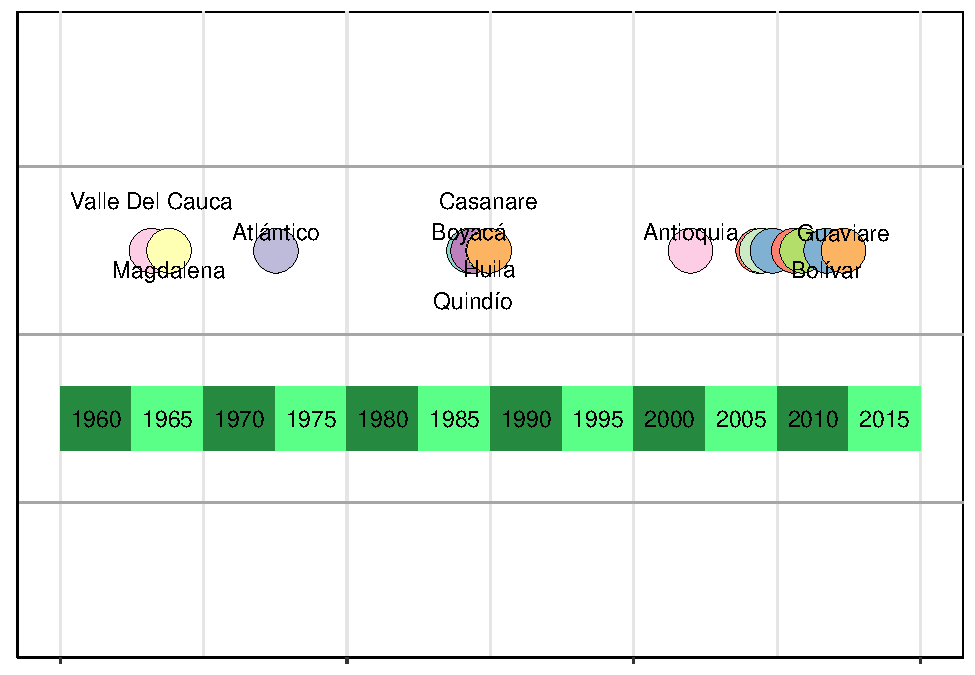
\includegraphics[width=1\linewidth]{InformeFinal_files/figure-latex/serieTiempoCreacion-1} 

}

\caption{Línea de tiempo de actas de creación de FRE.}\label{fig:serieTiempoCreacion}
\end{figure}

Más adelante, la creación de la Federación Nacional de Departamentos (FND) permitió a los departamentos con niveles de gobernanza mucho más simples, la creación y constitución de los FRE dentro del organigrama de las respectivas entidades del nivel departamental con funciones en salud. La autonomía administrativa, financiera y presupuestal de las entidades territoriales, el respeto a la pluralidad ideológica, la promoción del desarrollo integral y el respeto a la Constitución Política y a las leyes, son los principios de la FND. Además, las asesorías en las áreas jurídica, económica, financiera y administrativa, a cargo de la FND, facultaron a los departamentos con capacidades inferiores para la constitución de sus FRE. En este periodo de tiempo se logran ver distintos FRE creados, a partir de la fecha de creación de la Federación Nacional de Departamentos (FND) en 1994\textsuperscript{\protect\hyperlink{ref-FederacionNacionaldeDepartamentos2021}{5}}.

Sin embargo, también hay algunos territorios considerados ``grandes'', debido a su situación demográfica y desarrollo económico, cuyos FRE fueron creados en la primera parte de los años 2000. Estos casos particulares (p.ej. Antioquia, Santander, Norte de Santander, y Nariño), posiblemente se podrían explicar en función de la organización interna de cada dirección departamental de salud. Especialmente, hasta ese tiempo, aquellos departamentos mostraron un interés primigenio en regular la venta de estos productos en su territorio.

Particularmente en algunos territorios del país, no se cuenta con un FRE propiamente constituido, por medio de acto administrativo, suscrito por el gobernador. Por lo tanto, el control que se tiene sobre los medicamentos denominados Monopolio del Estado, lo ejercen a partir de su propia interpretación de la Resolución 1478 del 2006\textsuperscript{\protect\hyperlink{ref-MSPS1478-2006}{1}} y Resolución 1479 del 2006\textsuperscript{\protect\hyperlink{ref-MSPS1479-2006}{2}}. Durante las asistencias técnicas desarrolladas, se presentaron algunos casos como Córdoba y Vaupés en los cuales no fue posibles verificar el acto administrativo de creación.

\hypertarget{estructura-organizacional}{%
\section{Estructura organizacional}\label{estructura-organizacional}}

La estructura organizacional de los FRE departamentales es un elemento crítico para evaluar las condiciones y características actuales de cada ente territorial, en virtud de su capacidad para cumplir todas las funciones expuestas en el Artículo 2° de la Resolución 1479 del 2006. Por este motivo, en la Figura \ref{fig:perfilProfesionalEncargado} y \ref{fig:perfilProfesional2} se muestran los diferentes profesionales que conforman los equipos de trabajo de todos los FRE a nivel nacional.

En el panel izquierdo de la Figura \ref{fig:perfilProfesionalEncargado} se observa especialmente la distribución de los perfiles profesionales de los encargados de cada FRE departamental. Se evidencia que la mayoría de departamento cuentan con Químicos Farmacéuticos como responsables encargados de los entes territoriales. De manera similar, se observan Técnicos en Regencia en Farmacia ocupando este cargo a nivel territorial, cuyos perfiles permanecen en la misma línea profesional de trabajo, referente al conocimiento y habilidades en la gestión de los medicamentos. Lo anterior, tiene ventajas en los procesos internos del FRE, ya que permite un adecuado desarrollo de las funciones principales del ente territorial y la resolución de problemas técnicos es más probable.

Por otro lado, se evidencia un grupo de profesionales diferentes a los anteriores, pero denominados como profesionales de la salud, cuyas competencias pueden relacionarse de alguna manera con la adecuada administración y gestión de los medicamentos. Por el contrario, se deben resaltar (4) profesionales, encargados de algunos FRE, que no poseen este tipo de habilidades idóneas y apropiadas, desde su formación profesional, lo que podría resultar en dificultades técnicas para el desarrollo interno de las entidades territoriales.

Para el análisis del recurso humano de los FRE se tuvieron en cuanto dos clasificaciones:

\begin{itemize}
\item
  De acuerdo con sí la persona era la encargada del FRE o un apoyo del(a) encargado(a).
\item
  De acuerdo con la carga laboral relacionada con actividades del FRE. Se consideró como personal directo a aquel que desempeña más de un 50\% de su tiempo en actividades relacionadas al FRE y personal vinculado como aquel que desempeña menos del 50\% de su tiempo en estas actividades FRE.
\end{itemize}

\begin{figure}[b!]

{\centering 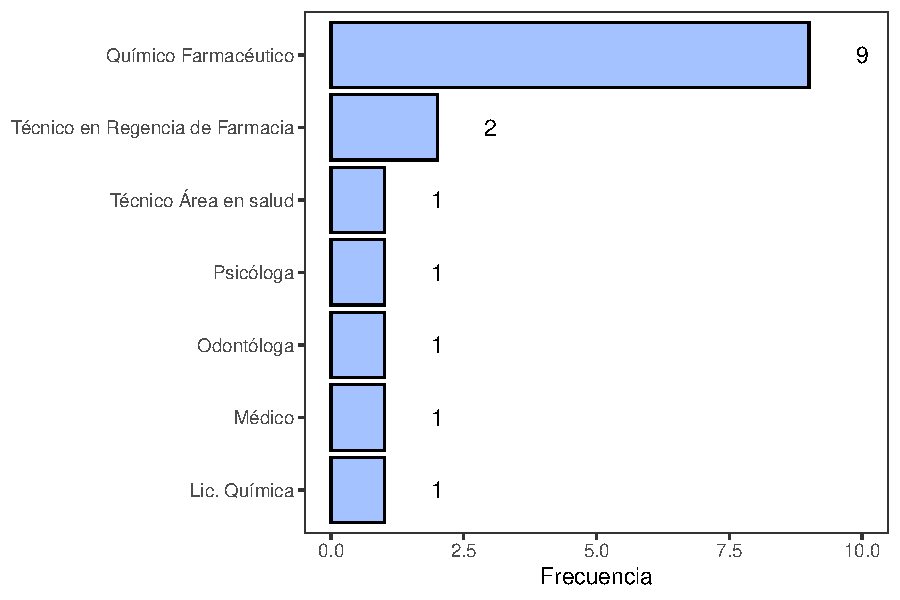
\includegraphics[width=1\linewidth]{InformeFinal_files/figure-latex/perfilProfesionalEncargado-1} 

}

\caption{Perfil de profesional de encargados de los FRE.}\label{fig:perfilProfesionalEncargado}
\end{figure}

En la Figura \ref{fig:perfilProfesional2} se observan los perfiles profesionales del personal de apoyo de los FRE a nivel nacional. Principalmente, se destaca una gran mayoría de Técnicos en Regencia en Farmacia (39) seguido de un grupo menor de profesionales Químicos Farmacéuticos (10), apoyando en las actividades de los FRE departamentales. Esto demuestra que gran parte de los entes territoriales están alineados con lo expuesto en el Artículo 3° de la Resolución 1479 del 2006\textsuperscript{\protect\hyperlink{ref-MSPS1479-2006}{2}}, donde mencionan que el Químicos Farmacéuticos y Tecnólogos en Regencia en Farmacia son profesionales considerados como personal calificado para el cumplimiento de las funciones requeridas por el FRE.

\begin{figure}[t!]

{\centering 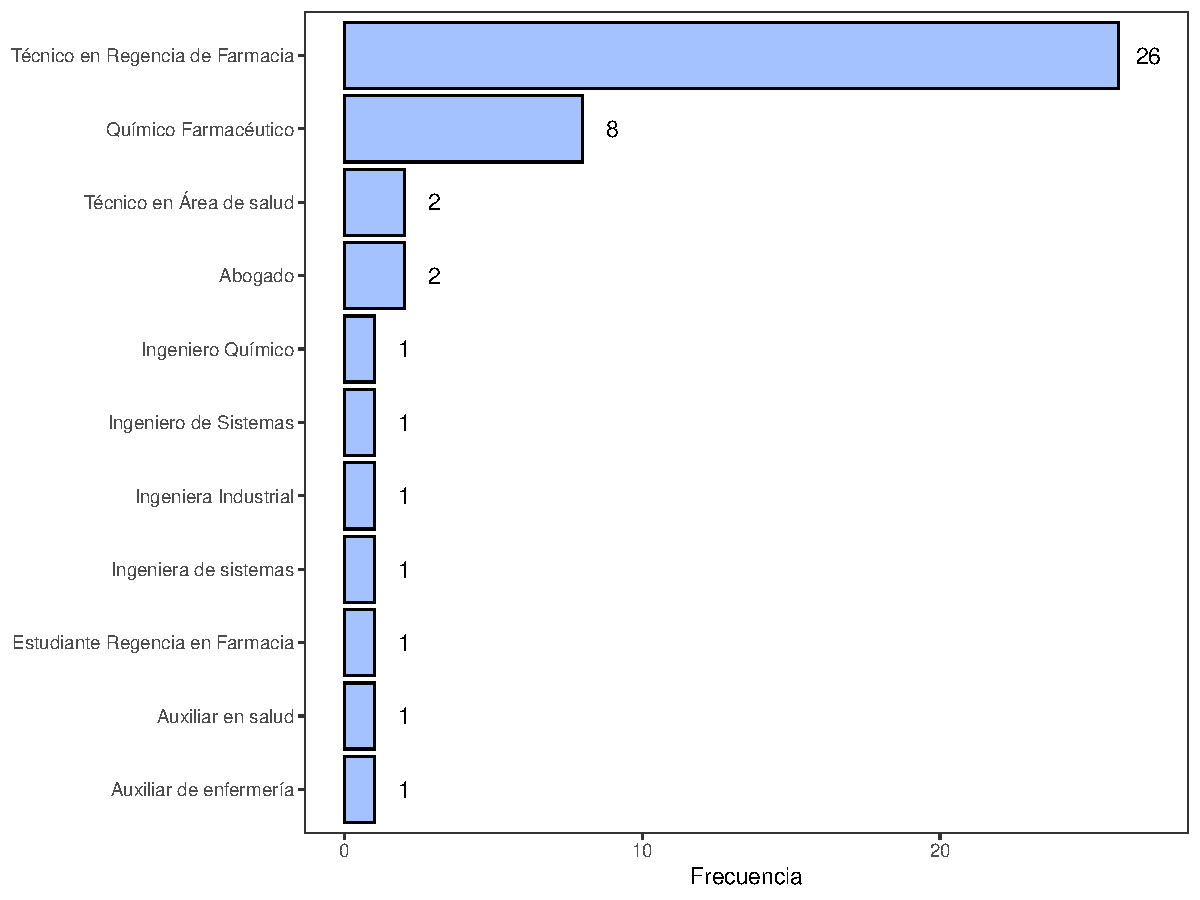
\includegraphics[width=0.9\linewidth]{InformeFinal_files/figure-latex/perfilProfesional2-1} 

}

\caption{Perfil de profesional de personal de apoyo a los FRE.}\label{fig:perfilProfesional2}
\end{figure}

Adicionalmente, la Figura \ref{fig:perfilProfesional2} también muestra otro tipo de profesionales de apoyo al encargado del FRE, diferente al personal calificado mencionado anteriormente. Este factor podría brindar ventajas al equipo de trabajo del FRE particularmente, en función de la multidisciplinariedad. La participación de distintas disciplinas puede entregar más conocimientos y alternativas en el desarrollo laboral interno de cada FRE departamental. No obstante, es importante aclarar que ningún FRE debería dejar de contar con la participación del personal calificado, estipulado en el Artículo 3° de la Resolución 1479 del 2006\textsuperscript{\protect\hyperlink{ref-MSPS1479-2006}{2}}.

El número de personas que trabajan en cada FRE, es otro elemento crítico para la evaluación de condiciones y características actuales de cada ente territorial, en virtud de su capacidad para cumplir todas las funciones expuestas en el Artículo 2° de la Resolución 1479 del 2006\textsuperscript{\protect\hyperlink{ref-MSPS1479-2006}{2}}. La Figura \ref{fig:perfilProfesional3} exhibe la frecuencia absoluta del número de personas que se encuentran vinculadas a los entes territoriales del país. Es decir, la cantidad de profesionales que conforman los equipos de trabajo de todos los FRE departamentales.

\begin{figure}[b!]

{\centering 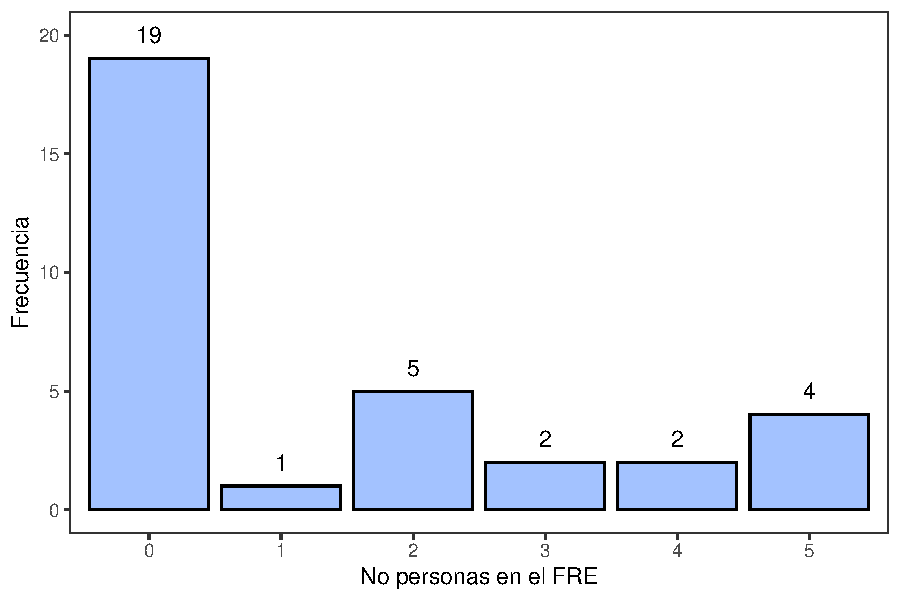
\includegraphics[width=1\linewidth]{InformeFinal_files/figure-latex/perfilProfesional3-1} 

}

\caption{N.° de personas que trabajan en el FRE. (A) Conteo de FRE por número de personas. (B) Mapa con número de personas por departamento.}\label{fig:perfilProfesional3}
\end{figure}

Según lo anterior, podemos evidenciar que no son muchas personas vinculadas a los FRE para conformar su equipo de trabajo. En su gran mayoría tienen únicamente hasta tres personas para el desempeño del FRE, contemplando que nueve FRE tienen solo 2 personas vinculadas. Son muy pocos entes territoriales que mantienen un grupo de trabajo grande con profesionales interdisciplinarios. La Figura \ref{fig:perfilProfesional3} exhibe de manera completa los datos que acompañan el análisis anterior.

El tipo de contrato que los diferentes entes territoriales emplean para vincular el personal es otro factor crítico en el cumplimiento de las funciones de los FRE. De acuerdo con lo anterior, la Figura \ref{fig:pieProfesional2} muestra la proporción del tipo de vinculación del personal del FRE a nivel nacional, diferenciándose entre personal directo y personal vinculado. Este último, tiene cierta exclusividad con el FRE al destinar más del 50\% en actividades de este, y de acuerdo a sus obligaciones contractuales, también adelanta otras actividades con otras dependencias de la dirección departamental de salud.

A partir de la Figura \ref{fig:pieProfesional2} se puede notar una gran tendencia que tienen todos los FRE a nivel nacional, referente al tipo de vinculación por medio de Contrato Por Prestación De Servicios (CPS). La gran mayoría, precisamente, el 98\%, del personal de apoyo de los FRE está relacionado con contratos CPS. Estas personas son vinculadas al ente territorial para cumplir algunas actividades internas del FRE, pero también tienen otras actividades laborales, fuera del FRE, según sus obligaciones contractuales. Por el contrario, el personal directo al funcionamiento del FRE, cuya atención es completa en las labores internas del FRE, está relacionado en su mayoría, por nombramiento, es decir, como servidor público. En muchos departamentos, la persona encargada del FRE es el único profesional nombrado, mientras que el resto del equipo de trabajo del FRE, guardan una predisposición para ser relacionados como contratistas, por medio de CPS.

\begin{figure}[t]

{\centering 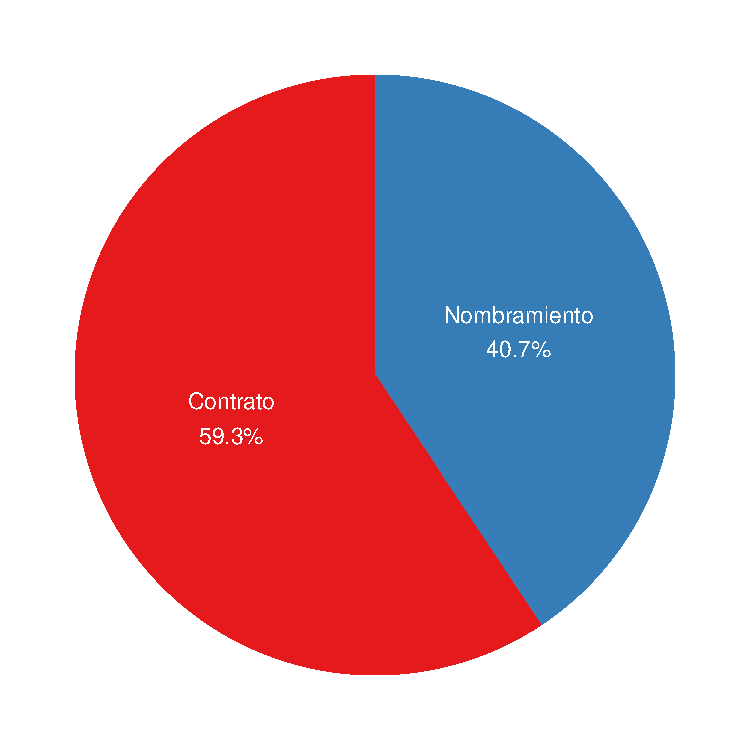
\includegraphics[width=0.85\linewidth]{InformeFinal_files/figure-latex/pieProfesional2-1} 

}

\caption{Tipo de vinculación al FRE.}\label{fig:pieProfesional2}
\end{figure}

La anterior tendencia puede interferir y generar inconvenientes en la continuidad del desarrollo adecuado del FRE, afectando la funcionalidad y abandonando algunas actividades críticas para el cumplimiento de sus objetivos de creación. En algunos casos, este tipo de personas vinculadas por CPS, dejan de laborar los primeros meses del año, ya que su contrato finalizó el año pasado, y debido a barreras administrativas, no son contratadas hasta el segundo bimestre del año. El personal nombrado en muchos casos es la persona encargada del FRE, cuyos temas operativos no están dentro de su cotidianidad y no son fáciles cumplirlos. Por tal motivo estas actividades operativas se dejan de hacer en el territorio hasta que sea contratado el personal de apoyo. Como es el caso de la consolidación de los informes que deben ser enviados mensualmente al FNE.

Adicionalmente, en la Tabla \ref{tab:CaracterizacionIngreso1} se observa la proporción del tipo de vinculación del personal del FRE, discriminado por cada región del país. A partir de esta información, se observa que en 5 regiones predomina la Contratación por Prestación de Servicios respecto al Nombramiento del personal del FRE. Además, se logra observar que en las regiones más alejadas de la capital Bogotá D.C., existe una prevalencia mucho más fuerte con esta CPS. Por consiguiente, los problemas mencionados anteriormente relacionados con la CPS, se pueden notar con mayor evidencia en estos territorios apartados del centro del país.

\begin{table}

\caption{\label{tab:CaracterizacionIngreso1}Proporción de personas contratadas por región}
\centering
\begin{tabular}[t]{lll}
\toprule
Región & Nombramiento & Contratación\\
\midrule
Amazonía & 21.43\% & 78.57\%\\
Caribe & 42.86\% & 57.14\%\\
Central & 41.38\% & 58.62\%\\
Eje Cafetero & 58.33\% & 41.67\%\\
Orinoquía & 45.45\% & 54.55\%\\
\addlinespace
Pacífico & 19.23\% & 80.77\%\\
\bottomrule
\end{tabular}
\end{table}

\hypertarget{instituciones-inscritas-en-el-fre}{%
\section{Instituciones inscritas en el FRE}\label{instituciones-inscritas-en-el-fre}}

El número de instituciones inscritas en los FRE de cada departamento, puede variar según las condiciones demográficas particulares en cada territorio. Lo anterior se puede ver plasmado en la siguiente Figura \ref{fig:institucionesInscritas}, donde se exhibe el número de inscritos en cada FRE departamental. A partir de esta información, se puede apreciar el ente territorial con mayor inscritos en su territorio, correspondiendo al FRE Antioquia con un total de 1054 inscritos. Luego se posiciona en segundo lugar el FRE Valle del Cauca con 570 inscritos. Particularmente, estos dos departamentos se mantienen en los primeros lugares de los departamentos más poblados en Colombia, exceptuando Bogotá D.C. y Cundinamarca, según los datos obtenidos por el DANE en el ``Censo Nacional de Población y Vivienda 2018''\textsuperscript{\protect\hyperlink{ref-DANE2021}{6}}.

\begin{figure}[t]

{\centering 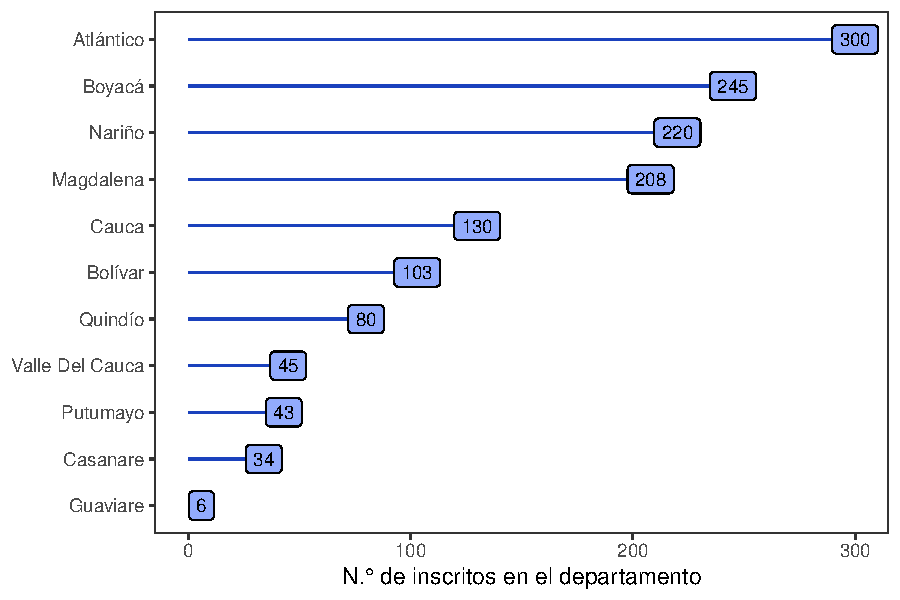
\includegraphics[width=0.9\linewidth]{InformeFinal_files/figure-latex/institucionesInscritas-1} 

}

\caption{N° de instituciones inscritas en el departamento.}\label{fig:institucionesInscritas}
\end{figure}

Los FRE que continúan en la lista de mayor número de inscritos, corresponden a los entes territoriales de Norte de Santander, Santander, Atlántico y Cesar, con un rango entre 298 y 358 inscritos territorialmente. Seguidamente, se encuentran los FRE departamentales Boyacá, Caldas, Nariño y Magdalena, con un rango de instituciones inscritas territorialmente ubicado entre 208 y 245. Por otro lado, los FRE con menor número de inscritos en su territorio son los FRE departamentales Guainía, Vichada, San Andrés, Amazonas, Vaupés, Arauca y Guaviare, considerándose los departamentos de Colombia con menor población en el país, según estadísticas del DANE\textsuperscript{\protect\hyperlink{ref-DANE2021}{6}}.

Por lo tanto, se puede determinar una relación directa entre los factores demográficos de cada territorio y el número de instituciones inscritas en cada FRE. Es decir, entre menos población habite en el departamento, menos instituciones se pueden encontrar en el territorio y así mismo son menos instituciones responsables de la gestión de MME.

Existe una relación demográfica en los departamentos sobre la cantidad de instituciones inscritas y los departamentos con más densidad de población. Lo anterior se explica de acuerdo cob la capacidad del departamento para atender la necesidad de MME en su población, en función del número de personas que integran el equipo de trabajo del ente territorial. En teoría, los FRE con mayor número de inscritos, deberían estar mucho más desarrollados para atender la necesidad de MME de su población local. No obstante, en las visitas técnicas se evidenció que el recurso humano de los FRE no da abasto con todas las tareas requeridas para su funcionamiento integral.

Un claro ejemplo de estas capacidades reducidas se puede evidenciar en el desempeño de cada FRE, referente a la entrega de informes mensuales al FNE. Actualmente existen varios FRE que cuentan con un recurso humano muy amplio, pero se quedan cortos con la entrega de estos informes al FNE, como es el caso del FRE Caldas, que pese a tener una cantidad de colaboradores por encima de la media, tiene un rezago importante en la entrega de informes de consumo de medicamentos al FNE. Por consiguiente, se puede deducir que el número de personas vinculadas al FRE no comprende una garantía en el cumplimiento de todas las funciones del FRE.

También se puede observar que la distribución geográfica de las regiones no se puede relacionar con la puntualidad en el envío de informes, tomando por ejemplo el caso de la región pacífico que está compuesta por Valle del Cauca, Cauca, Chocó y Nariño. Los departamentos de Valle del Cauca y Nariño tienen una alta densidad poblacional y en la Figura \ref{fig:institucionesInscritasRelacion} también se puede observar que están respectivamente por encima y por debajo de la media en el recurso humano que tienen para su funcionamiento y son quienes envían informes de manera puntual al FNE, mientras que el departamento del Cauca supera en recurso humano a Nariño por más del doble de personal y existe un importante atraso en el envío de estos informes, posiblemente sean factores externos cómo los tipos de contratación u otras responsabilidades adquiridas por parte de los coordinadores de los FRE en su territorio.

\begin{figure}[t]

{\centering 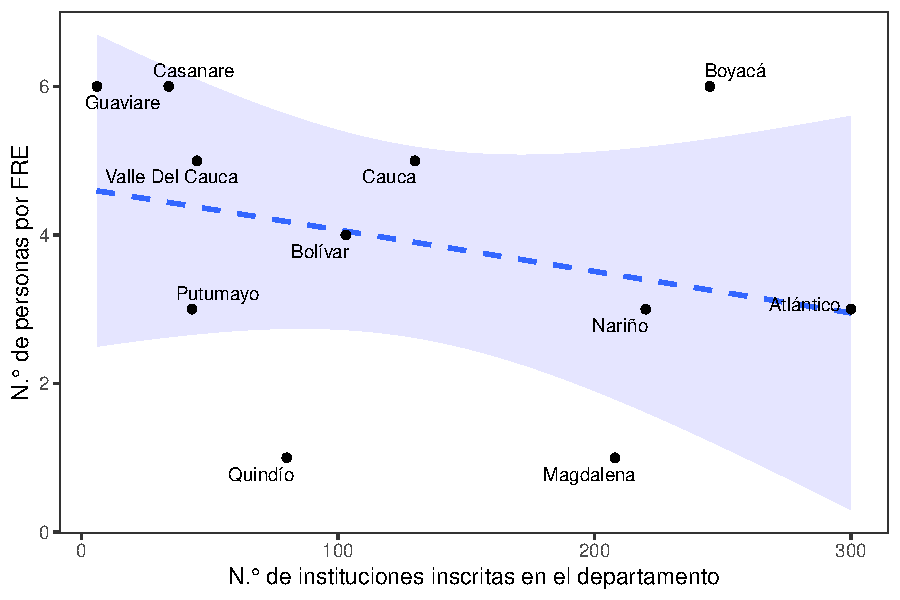
\includegraphics[width=0.85\linewidth]{InformeFinal_files/figure-latex/institucionesInscritasRelacion-1} 

}

\caption{Relación entre N.° de instituciones inscritas y personal del FRE.}\label{fig:institucionesInscritasRelacion}
\end{figure}

En la Figura \ref{fig:institucionesInscritasVARdemo} se puede determinar una relación directa entre la cantidad de instituciones inscritas y variables relacionadas a la demografía de cada departamento. Lo anterior se explica con la densidad demográfica del departamento y la necesidad de servicios de atención en salud cada vez más complejos. En teoría, los FRE con mayor número de inscritos de mayor complejidad, deberían estar mucho más desarrollados para atender la necesidad de MME de su territorio. Como es el caso del FRE Antioquia, cuyo departamento presenta un alto número de establecimientos inscritos y un nivel de complejidad alta en las instituciones, aumentando proporcionalmente el consumo de MME.

\begin{figure}[t!]

{\centering 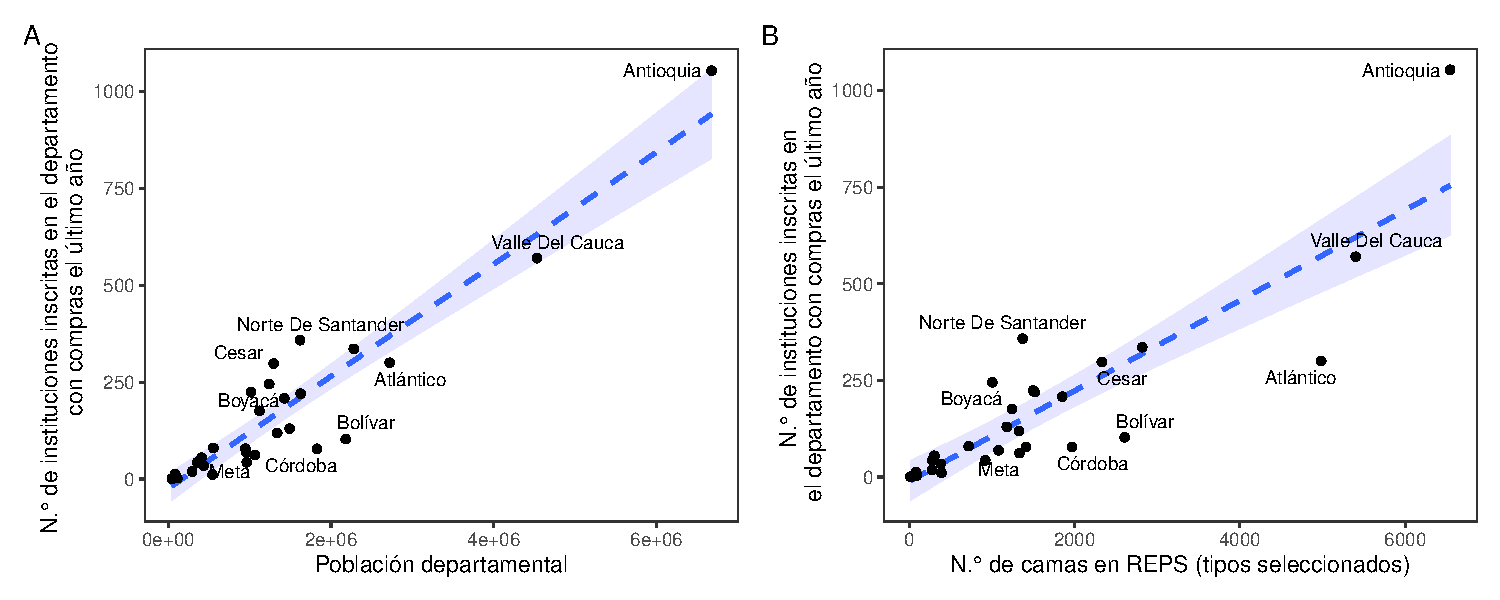
\includegraphics[width=1\linewidth]{InformeFinal_files/figure-latex/institucionesInscritasVARdemo-1} 

}

\caption{Relación de N.° de instituciones inscritas en el FRE con: (A) tamaño de la población en el departamento o (B) N.° de camas de acuerdo a REPS.}\label{fig:institucionesInscritasVARdemo}
\end{figure}

En la Figura \ref{fig:institucionesInscritasVARdemo}B se encuentra la relación directa entre el N.° de inscritos en el departamento y el número de camas (adultos, intermedio adulto, intensivo adulto, agudo mental, intermedio mental, salud mental), servicios de farmacodependencia y ambulancias medicadas de acuerdo al REPS\textsuperscript{\protect\hyperlink{ref-DireccionPrestaciondeServiciosyAtencionPrimaria2021}{7}} presentes en el departamento.

\hypertarget{caracterizaciuxf3n-de-las-fuentes-de-ingresos-de-los-fre}{%
\section{Caracterización de las fuentes de ingresos de los FRE}\label{caracterizaciuxf3n-de-las-fuentes-de-ingresos-de-los-fre}}

Para analizar las fuentes de ingreso que poseen los diferentes FRE departamentales, se debe tener en cuenta la posición del FRE dentro del organigrama de cada dirección departamental en salud. El análisis de las fuentes de ingresos de los FRE, en este punto, se hará exclusivamente con la información recolectada a partir del instrumento de encuesta que se usó para la recolección de información pertinente en este informe.

Cómo antecedente en el análisis, se entiende según las definiciones de la Resolución 1478 del 2006\textsuperscript{\protect\hyperlink{ref-MSPS1478-2006}{1}}, que un Fondo Rotatorio de Estupefacientes es:

\begin{quote}
\emph{``La Oficina encargada dentro de la Secretaría, Instituto o Dirección de Salud a nivel departamental, que ejerce la vigilancia, seguimiento y control a las entidades públicas, privadas y personas naturales que procesen, manipulen, sinteticen, fabriquen, distribuyan, vendan, consuman, dispensen sustancias sometidas a fiscalización y medicamentos que las contengan; así como garantizar la disponibilidad de medicamentos Monopolio del Estado a través de la dispensación y distribución en su jurisdicción y las demás funciones que le sean asignadas por el Ministerio de la Protección Social, o la institución competente.''}
\end{quote}

Por lo tanto, es una dependencia del ente territorial y no goza de autonomía administrativa o financiera cómo para ser considerada una Unidad Administrativa Especial, cómo si lo es el Fondo Nacional de Estupefacientes con sede en Bogotá, sin embargo, de acuerdo al Artículo 3 de la Resolución 1479 del 2006, los FRE\textsuperscript{\protect\hyperlink{ref-MSPS1479-2006}{2}}:

\begin{quote}
\emph{``{[}\ldots{]} deben tener una cuenta específica denominada ``Fondo Rotatorio de Estupefacientes'' para manejar sus operaciones. Las utilidades que se obtengan sólo podrán emplearse, para su administración, mejoras de dotación, buen funcionamiento del mismo y ejecutar programas contra la farmacodependencia y toxicología que adelante el Gobierno Nacional.''}
\end{quote}

De modo que la normativa interna de cada departamento podría entrar en conflicto con la misma resolución anteriormente citada que define las funciones y capacidades de los FRE, pudiendo generar bloqueos o demoras en determinados procesos internos que permitan un funcionamiento integral en el manejo de los MME.

Hecho este primer paso sobre entender de manera sucinta la relación que tienen los FRE con sus respectivas entidades territoriales, se puede comenzar a hacer el análisis de las gráficas con los resultados del instrumento de encuesta realizado.

\begin{figure}[t]

{\centering 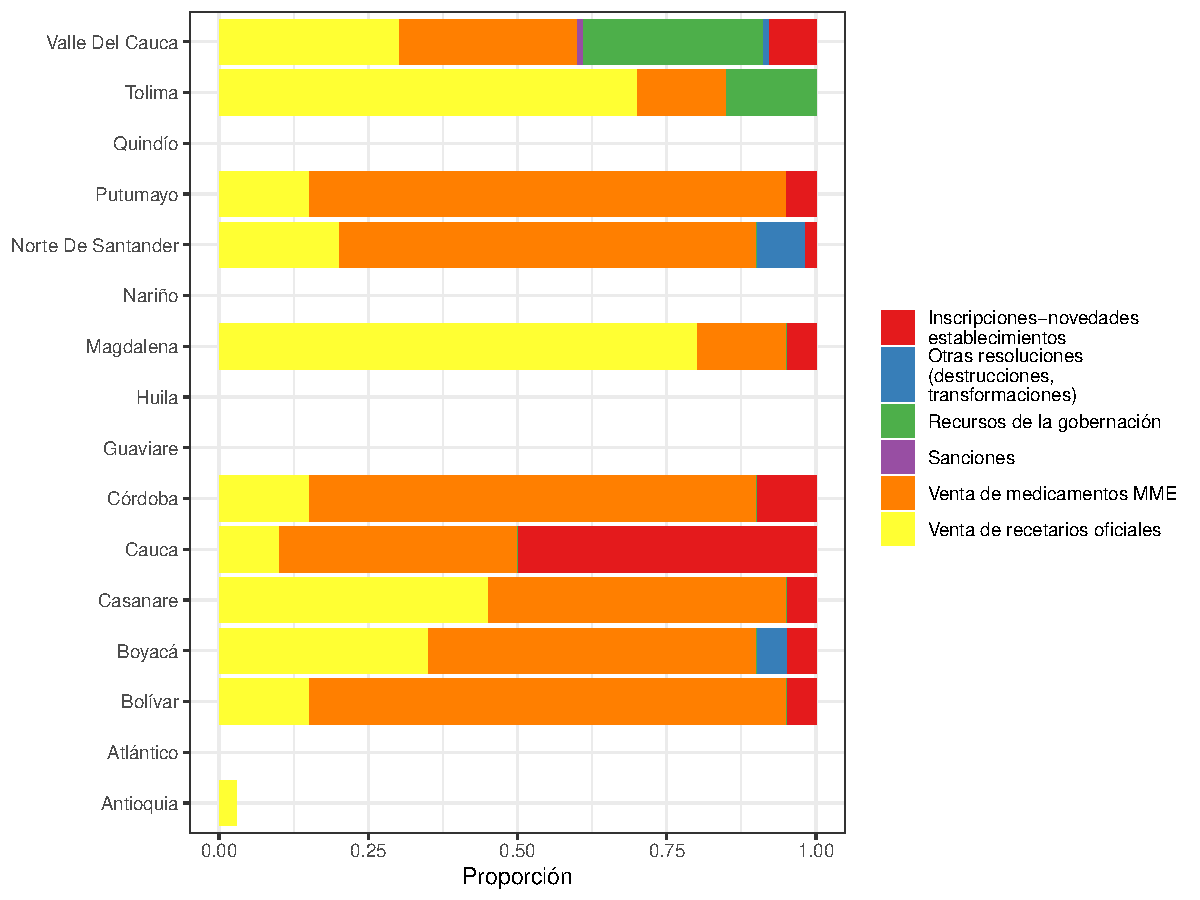
\includegraphics[width=0.85\linewidth]{InformeFinal_files/figure-latex/IngresosFRE1-1} 

}

\caption{Proporción de fuentes de ingresos de los FRE}\label{fig:IngresosFRE1}
\end{figure}

La Figura \ref{fig:IngresosFRE1}, nos muestra la proporción de los ingresos del FRE en sus cuentas bancarias, en base a las que serían sus principales actividades, cómo lo son:

\begin{itemize}
\item
  Venta de Medicamentos Monopolio del Estado
\item
  Venta de Recetarios Oficiales
\item
  Producción y emisión de actos administrativos pertinentes al manejo de MME
\item
  Inspección, Vigilancia y Control de Instituciones que manejen MCE
\end{itemize}

Aunque también los FRE pueden recibir recursos por parte de la gobernación o por parte del FNE.

En la Figura \ref{fig:IngresosFRE1} se observa que una tendencia a que la proporción de ingresos más grande es aquella que reciben los FRE departamentales por la venta de MME. Esto se puede deber a que cada departamento maneja independencia en los precios de venta de estos medicamentos y desde ahí se podría obtener una rentabilidad importante. En el desarrollo del apartado \protect\hyperlink{precioMedicamentos}{6.4 Precio de medicamentos} del presente informe, se desglosará un análisis más profundo sobre los precios de venta de los MME por departamento, pero a \emph{grosso modo} se puede notar que el margen es lo suficientemente alto para abarcar el porcentaje mayoritario de ingresos.

Particularmente, en la Figura \ref{fig:IngresosFRE2} se observa que en algunos departamentos cómo Magdalena, Atlántico o Tolima, la venta de recetarios oficiales es el ingreso más prominente del FRE. Así mismo, en todos los demás departamentos representa un ingreso importante para el ente territorial, aunque no sea la principal fuente de ingreso. A nivel nacional, esta fuente de ingreso carga con una parte muy importante del erario de cada FRE departamental. Con la desaparición de los recetarios oficiales físicos en el mediano plazo, es necesario generar alternativas económicas para subsanar este recurso que desaparecería y adecuar estrategias financieras para el auto sostenimiento de cada FRE.

\begin{figure}[th!]

{\centering 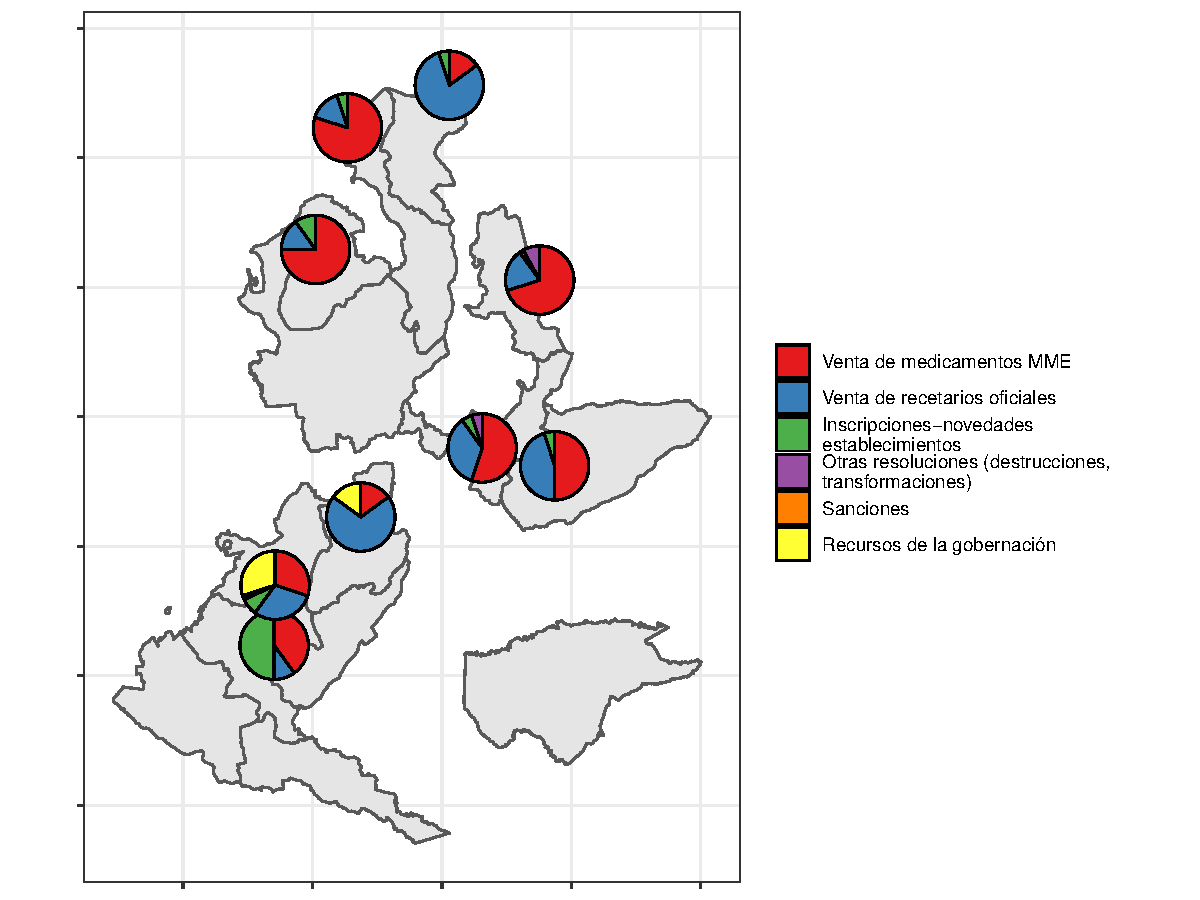
\includegraphics[width=0.85\linewidth]{InformeFinal_files/figure-latex/IngresosFRE2-1} 

}

\caption{Mapa con fuentes de ingresos de los FRE.}\label{fig:IngresosFRE2}
\end{figure}

\hypertarget{clasificaciuxf3n-de-los-fre-por-nivel-de-complejidad}{%
\section{Clasificación de los FRE por nivel de complejidad}\label{clasificaciuxf3n-de-los-fre-por-nivel-de-complejidad}}

A partir de las visitas técnicas desarrolladas en cada territorio, se lograron observar notorias diferencias entre los FRE departamentales. Esto se podría explicar por las diferencias administrativas y factores demográficos que tiene cada departamento. Esto permite que cada FRE se desenvuelva en determinada forma y esto resulta en el grado de eficiencia que presenta el ente territorial, para el manejo de MME en la región.

Según lo anterior, se propone una clasificación de los FRE, de acuerdo a su nivel de complejidad, sin el ánimo de juzgar el trabajo desarrollado en cada territorio. Esta sección procura por reconocer y clasificar los FRE en grupos, conforme a sus capacidades actuales y similaridad entre departamentos. Lo anterior con el fin de generar un instrumento que sirva como insumo para la generación de políticas públicas y toma de decisiones relacionadas con el manejo de MME.

A continuación, se presenta la descripción de las 5 variables definida para la clasificación de los FRE, cuya agrupación contempla el nivel de complejidad del ente territorial:

\begin{itemize}
\item
  Presupuesto departamento (general y sector salud).
\item
  Número de instituciones inscritas en el departamento.
\item
  Proporción de adquisición de MME (proporción de portafolio).
\item
  Número de compras directas de instituciones en el departamento al FNE (entendidas como una desviación de la cadena de suministro).
\item
  Proporción de meses con entrega del Anexo 1 de la Resolución 1479 de 2006 (cumplimiento).
\item
  Proporción de meses con entrega del Anexo 2 de la Resolución 1479 de 2006 (cumplimiento).
\end{itemize}

Muchas variables fueron tomadas de forma externa a la encuestas teniendo en cuenta la información disponible en cada una de ellas, con el fin de visualizar el estado actual de cada FRE, considerando distintos factores internos y externos que tienen las entidades territoriales. Esto permite que la distribución y clasificación de los FRE sea más robusta, ya que está contemplando la mayor realidad posible en cada territorio, para el momento de este análisis.

Es importante resaltar que la complejidad concluida estaría relacionada con la capacidad que tiene el FRE de cumplir con sus funciones y responsabilidades, considerando factores económicos propios del departamento. Un ejemplo ilustrativo corresponde al FRE Córdoba, donde el ente territorial es clasificado en la categoría \emph{``FRE altamente consolidado''}. A pesar de esta clasificación, el rubro económico destinado para temas de salud en este departamento es relativamente bajo, sin embargo, el personal del FRE procura realizar una buena gestión estos recursos para el adecuado manejo de MME y recetarios oficiales.

En primer lugar, la variable de presupuesto y número de inscritos, refleja la asignación de recurso económico en cada región para la partida presupuestal de los temas en salud de cada territorio. Esto entendiéndose como un condicionante de la capacidad que tienen los FRE para disponer de infraestructura tecnológica y recurso humano suficiente, para cumplir todas sus funciones como ente territorial. Adicionalmente, el número de inscritos en cada territorio muestra la complejidad de la oferta y demanda en cada región, la cual debe satisfacer la gestión del FRE.

La variable referente a la proporción de adquisición de MME, indica la proporción de medicamentos ofertados por el FRE en su territorio, de acuerdo con el portafolio general de MME presentado por el FNE. A partir de esto, se determina de manera indirecta, la capacidad de manejo de portafolio que tiene un FRE. Esta capacidad de manejo está relacionada con las condiciones de almacenamiento, infraestructura física y recurso humano disponible en el ente territorial.

Otra variable importante en este análisis es la variable referente a cantidad de compras directas al FNE. Esta información refleja el número de compras que realizaron las instituciones inscritas en cada territorio con el FNE, debido al desabastecimiento de MME en su respectivo departamento. Esto podría ser causa de una proyección de compra de MME inapropiada, por parte del FRE, cuyo proceso está directamente relacionado con los anexos técnicos de distribución y consumo que son presentados mensualmente.

Finalmente, las variables relacionadas con el cumplimiento de entrega del Anexo 1 y Anexo 2 de la Resolución 1479 de 2006\textsuperscript{\protect\hyperlink{ref-MSPS1479-2006}{2}}, fueron incluidas en esta clasificación, ya que inciden en gran proporción en la proyección de adquisición de MME para satisfacer las necesidades del territorio. La consolidación de la información dispuesta en estos anexos se relaciona directamente con la cantidad de personas vinculadas al FRE, cuyo factor muestra la capacidad de recurso humano en cada FRE.

Para ilustrar el comportamiento de los FRE respecto a las variables seleccionadas se realizó un análisis de componentes principales (PCA, \emph{Principal Component Analysis}). La Figura \ref{fig:PCA1} muestra el comportamiento de las 5 variables definidas para este análisis respecto a los componentes principales. En primer lugar, se puede determinar que las variables más próximas en el plano del componente 1 (PC1), presentan la mayor variabilidad entre los FRE, seguido por aquellas ubicadas cerca del plano del componente 2 (PC2). Las variables de monto presupuestal (general y salud), así como número de inscritos y en cierta medida la proporción del portafolio tienen un alta correlación entre sí por lo cual presentan una proyección cercana entre sí.

\begin{figure}[t]

{\centering 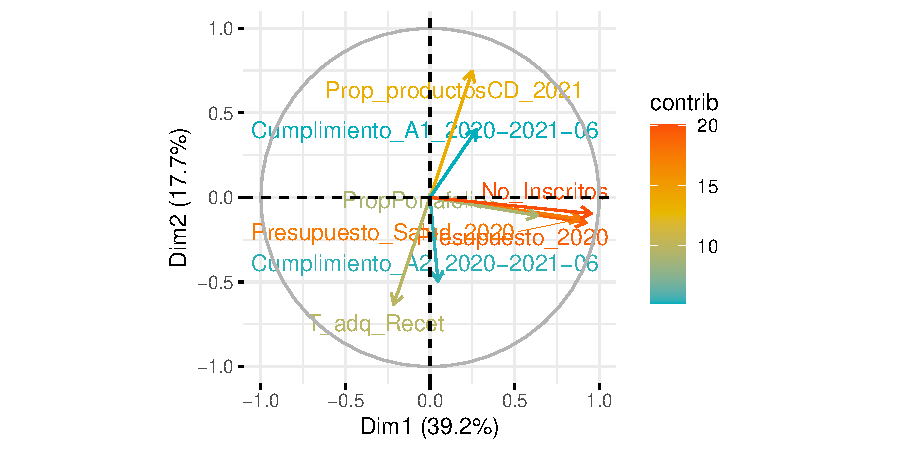
\includegraphics[width=0.9\linewidth]{InformeFinal_files/figure-latex/PCA1-1} 

}

\caption{Variables involucradas en la construcción de los componentes principales}\label{fig:PCA1}
\end{figure}

Por el contrario, las variables más dispersas en el plano presentado en la Figura \ref{fig:PCA1}, no guardan relación entre sí, por lo tanto, estas variables tienen información importante para realizar la clasificación de los FRE. En este orden de ideas, la variable referente a la consolidación del anexo 2 en los FRE no mantiene una relación directa con el número de compras directas que haya hecho el departamento o con la variable del portafolio que ofrecen los FRE.
Se realizó un análisis de agrupación (\emph{cluster}) jerárquico mediante el algoritmo de Ward en el software R. Se seleccionaron 5 grupos de acuerdo al análisis mediante un criterio de \emph{codo}. A partir de la descripción anterior, la clasificación según la complejidad de los FRE, resultó como aparece en la Figura \ref{fig:PCA1-2}.

\begin{figure}[t]

{\centering 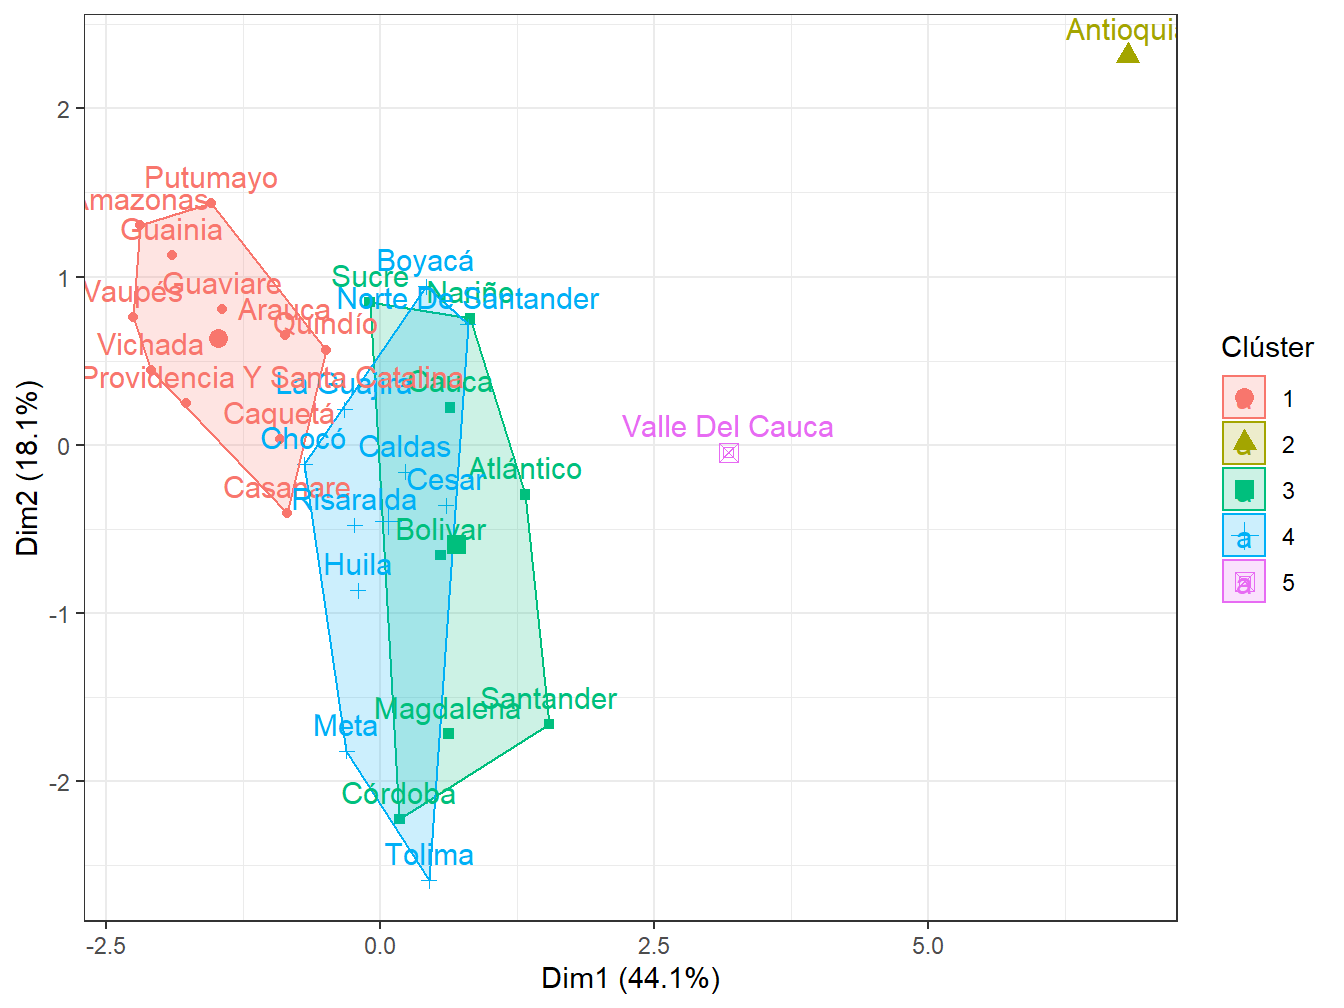
\includegraphics[width=0.9\linewidth]{InformeFinal_files/figure-latex/PCA1-2-1} 

}

\caption{Clasificación de los FRE en grupos de acuerdo a análisis por clúster}\label{fig:PCA1-2}
\end{figure}

Luego de un análisis multivariado en el lenguaje de programación R, se definieron varios parámetros a tomar en cuenta para esta clasificación. Según los datos obtenidos por las 5 variables en cada departamento, se lograron agrupar los FRE en 3 categorías, las cuales serán descritas a continuación:

\begin{itemize}
\item
  FRE suficientemente consolidado (Verde)
\item
  FRE medianamente consolidado (Azul)
\item
  FRE en proceso de consolidación (Rojo)
\end{itemize}

Es preciso resaltar que los FRE Antioquia y Valle del Cauca fueron categorizados como dos categorías distintas, respectivamente. Lo anterior es suscitado por las grandes diferencias en la gestión de MME y la administración departamental, que tienen estos entes territoriales frente a los otros FRE. No obstante, el análisis descriptivo de la Figura \ref{fig:PCA1-2}, permite organizar estas agrupaciones en 3 categorías, dejando fuera a estos dos FRE, cuyas capacidades exceden la media de la gestión de los FRE a nivel nacional.

La categoría \emph{``FRE suficientemente consolidado''} exhibida en color verde en la Figura \ref{fig:PCA1-2}, habla de un FRE que tiene capacidades operativas y administrativas suficientes, teniendo en cuenta factores externos como el presupuesto y la complejidad de las instituciones inscritas en su territorio. Sin embargo, existen variables donde se requiere adelantar un trabajo profundo para llegar a tener una gestión ideal como el caso de Antioquia y Valle del cauca, recalcando que también son territorios de alta complejidad. Es necesario aclarar que esta denominación ``altamente consolidado'' está relacionada directamente con las capacidades del departamento, para gestionar sus recursos en salud.

La categoría \emph{``FRE medianamente consolidado''} se muestra de color azul en la Figura \ref{fig:PCA1-2} Esta clasificación representa a los FRE que cumplen con las necesidades de manejo de MME en su territorio, no obstante, estos entes territoriales tienen suficiente presupuesto para adelantar una gestión aún mejor y más robusta. Por este motivo se recomienda a los FRE de este grupo, mejorar en los siguientes temas puntuales como: (i) contratación del personal del FRE, (ii) cumplimiento de los anexos de la Resolución 1479 de 2006 y (iii) proyección adecuada del consumo de MME en cada territorio.

La categoría \emph{``FRE en proceso de consolidación''} exhibida en color rojo en la Figura \ref{fig:PCA1-2}, contiene a los FRE que necesitan asistencia técnica inmediata por parte del FNE, de la mano de su respectiva Dirección Departamental de salud. Lo anterior se debe a que estos FRE no presentan una complejidad muy alta en función de las pocas instituciones inscritas, densidad demográfica y el limitado portafolio de MME que se distribuyen en estos territorios.
En adición, el seguimiento y manejo de los MME es débil en estos FRE y sus herramientas tecnológicas son limitadas. Por esta razón, la asistencia técnica por parte del FNE puede ser de gran ayuda, para entender cómo distribuir los recursos a disposición del FRE y mejorar en capacidades propias, con el fin de apoyar en el proceso de consolidación del FRE.s

\hypertarget{recetarios-oficiales}{%
\chapter{Recetarios oficiales}\label{recetarios-oficiales}}

\maxdeadcycles=1000

La prescripción de un medicamento es el acto que realiza un médico para indicar el inicio de un tratamiento terapéutico. En Colombia, dicha prescripción debe hacerse por escrito, previa evaluación del paciente y registro de sus condiciones y diagnóstico en la historia clínica, utilizando para ello la Denominación Común Internacional (nombre genérico) y cumpliendo los requisitos descritos en el Decreto 2200 de 2005, Artículo 16 y Artículo 17\textsuperscript{\protect\hyperlink{ref-MSPS2200-2005}{8}}.

Bajo los parámetros establecidos anteriormente, se crea el recetario oficial, que es un documento oficial avalado por la entidad competente, es de carácter personal e intransferible para uso de los prescriptores de salud en la formulación de los MCE y MME. La prescripción de medicamentos de control especial para uso humano o veterinario solo se podrá efectuar en los recetarios oficiales suministrados por los FRE, para médicos en ejercicio legal de su profesión y/o por el Consejo Profesional de Medicina Veterinaria y Zootecnia de Colombia (Comvezcol) para médicos veterinarios y médicos veterinarios zootecnistas. Los profesionales que laboren en las instituciones podrán hacer uso del Recetario Oficial adquirido por la entidad\textsuperscript{\protect\hyperlink{ref-MSPS1478-2006}{1}}.

Los FRE de las Secretarías, Instituciones o Direcciones Departamentales de Salud, y/o Comvezcol para médicos veterinarios, son los únicos autorizados para emitir, distribuir y vender el Recetario Oficial para la prescripción\textsuperscript{\protect\hyperlink{ref-MSPS1478-2006}{1}}.

\hypertarget{existencia-de-recetarios}{%
\section{Existencia de recetarios}\label{existencia-de-recetarios}}

\hypertarget{existencias-en-el-fre}{%
\subsection{Existencias en el FRE}\label{existencias-en-el-fre}}

En el marco de las Jornadas de inmersión territoriales con los FRE del país se pudo determinar la cantidad de recetarios oficiales con los que cuentan entre los meses de junio a septiembre. Así pues, como se observa en la Figura \ref{fig:existenciasRecetarios}A, se observa la tendencia de los departamentos más distantes de la capital de la nación, a presentar una menor cantidad de recetarios en existencia.

\begin{figure}

{\centering 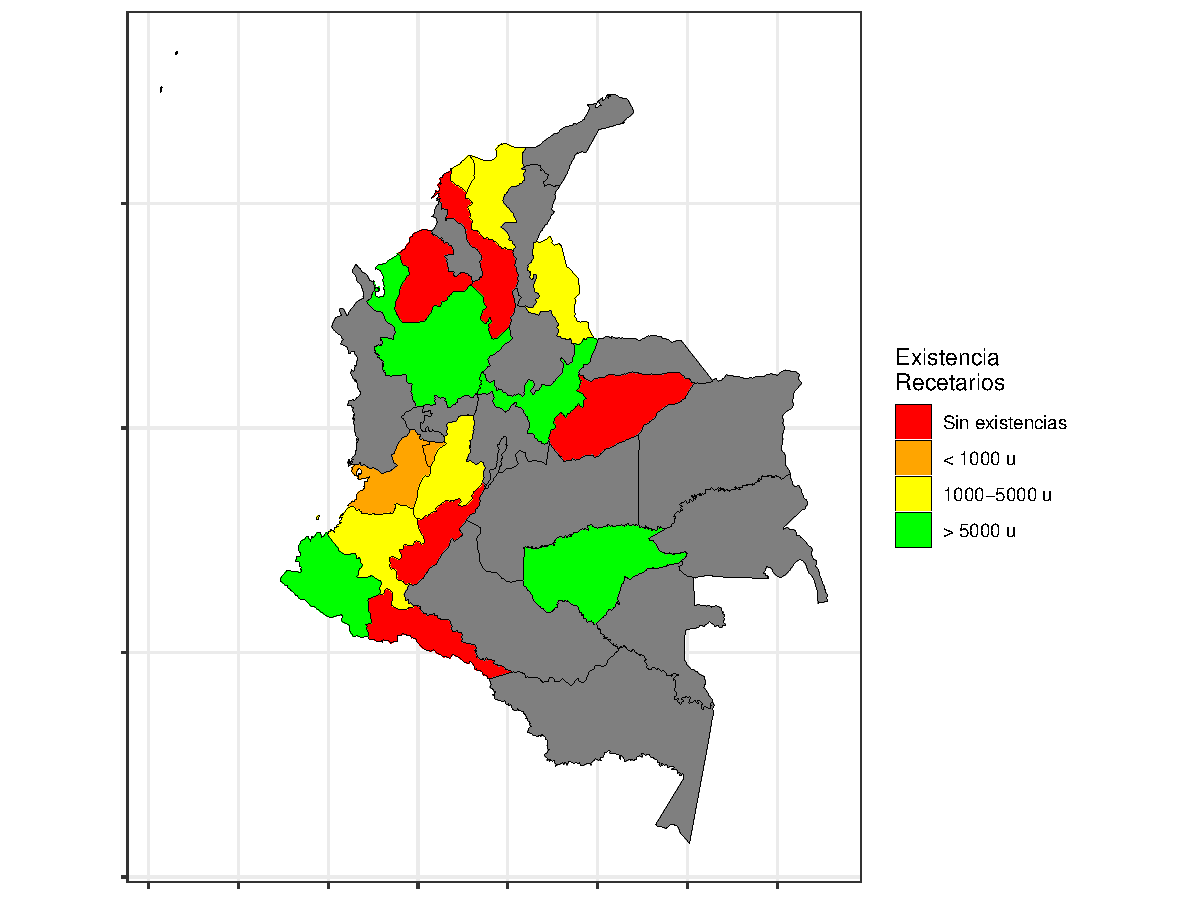
\includegraphics[width=1\linewidth]{InformeFinal_files/figure-latex/existenciasRecetarios-1} 

}

\caption{Existencias de recetarios en el FRE. (A) N.° de existencias de recetarios en el FRE y (B) Cobertura de existencias de recetarios en el FRE.}\label{fig:existenciasRecetarios}
\end{figure}

En los extremos norte y sur, es decir, la región Caribe y Amazónica se tiene la mayor proporción de inexistencias de recetarios, en comparación con el resto de las regiones. El motivo de esto puede ser la dificultad para encontrar empresas de fabricación adecuada de documentos con características particulares como lo son los recetarios oficiales, por los cuales, en algunos departamentos limítrofes se contratan empresas de departamentos del interior, dado que en sus regiones no existe la capacidad para elaborarlos. Por otro lado, los FRE más antiguos y consolidados son los que en el presente disponen de mayor cantidad de recetarios, lo que puede estar influenciado, igualmente por la cercanía y facilidad de contratación con empresas de la región.

Dentro del censo realizado en los diferentes departamentos del país, se observa en la Figura \ref{fig:existenciasRecetarios}B predisposición entre los distintos FRE a presentar en estos momentos una duración de existencias de recetarios oficiales a 25 semanas. El motivo de esto es que en gran parte de los entes territoriales se concretan órdenes de compra de recetarios por un año, de modo que en la época en la cual se realizó el censo, aproximadamente mitad de año, aún quedan alrededor de 20 a 30 semanas más para la finalización del año calendario. Además de ello, en ocasiones se estima un periodo de 2 a 3 meses más, es decir, disponibilidad de recetarios hasta febrero o marzo, ya que por motivos de contratación de personal a inicio del año calendario se dificulta llevar a cabo el proceso de licitación de recetarios hasta que se hayan contratado nuevamente a los funcionarios del FRE, cuestión que se da por el tipo de contrato laboral con el que están vinculados la mayoría de los funcionarios de apoyo en el país (Figura \ref{fig:pieProfesional2}).

Se tiene que Boyacá y Nariño son los departamentos que en la actualidad cuentan con mayor proyección de disponibilidad de recetarios oficiales ya que son regiones en donde el FRE hace compras para 2 a 3 años, procesos que fueron llevados a cabo recientemente, a inicio del año 2021.

\hypertarget{circulaciuxf3n-en-el-departamento}{%
\subsection{Circulación en el departamento}\label{circulaciuxf3n-en-el-departamento}}

Así mismo, ligado a las existencias actuales de recetarios oficiales en la nación, como se observa en la Figura \ref{fig:existenciasRecetarios2}, los departamentos en donde se presenta menor circulación de recetarios precisamente son los departamentos distantes del interior. Este fenómeno puede ser ocasionado por la baja densidad poblacional de dichos territorios, es decir, la rotación de recetarios oficiales en Antioquia, que es un departamento que cuenta con más de 5 millones de habitantes es la más alta ya que su población actual supera a la de los demás departamentos que cuentan con recetarios oficiales\textsuperscript{\protect\hyperlink{ref-DANE2021}{6}}.

\begin{figure}

{\centering 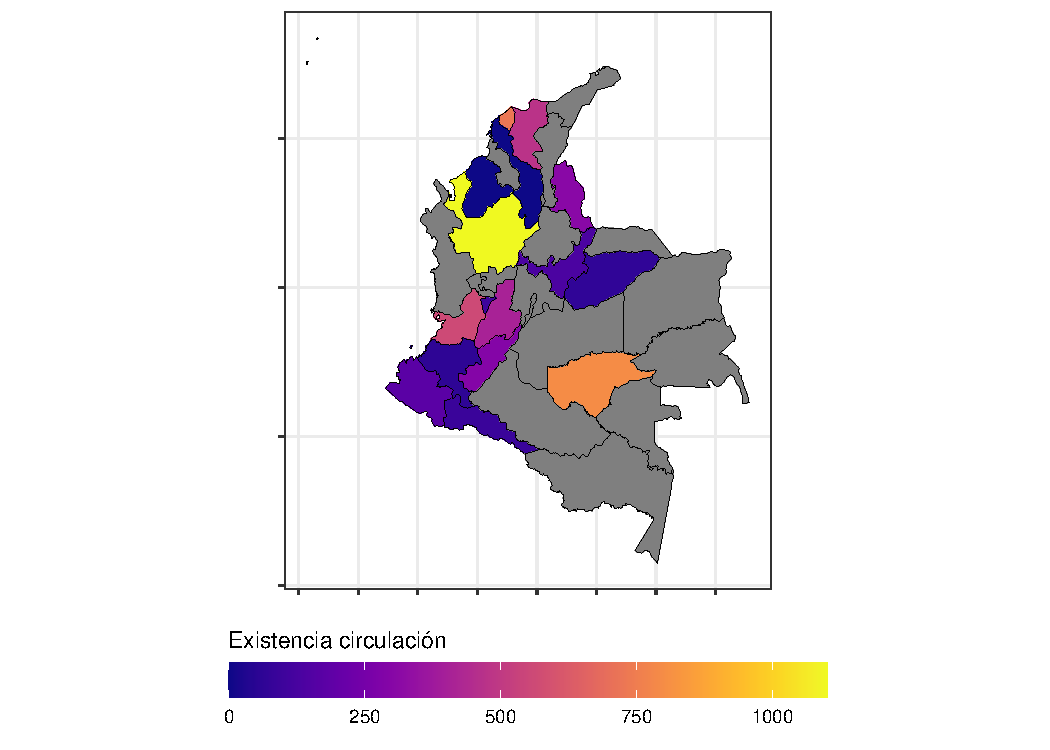
\includegraphics[width=0.85\linewidth]{InformeFinal_files/figure-latex/existenciasRecetarios2-1} 

}

\caption{N.° de recetarios circulantes en el departamento.}\label{fig:existenciasRecetarios2}
\end{figure}

\hypertarget{costos-de-recetarios}{%
\section{Costos de recetarios}\label{costos-de-recetarios}}

\maxdeadcycles=1000

\hypertarget{comparaciuxf3n-de-costos-y-precios-de-ventas-de-recetarios}{%
\subsection{Comparación de costos y precios de ventas de recetarios}\label{comparaciuxf3n-de-costos-y-precios-de-ventas-de-recetarios}}

Dentro del estudio de costos realizado se comparó el costo de compra del recetario contra su precio de venta. Así pues, se determinó que dentro del territorio el costo de los recetarios ronda entre los 10.000 COP y los 20.000 COP, con territorios como Valle del Cauca y Casanare, en donde dicho costo se aproxima a 30.000 COP. En algunos departamentos no se conocen los costos de adquisición de recetarios (Figura \ref{fig:costoRecetario}A), dada sus particularidades en la contratación, puesto que se encargan del proceso de licitación y contratación de recetarios, únicamente realizan estudios de necesidad que son enviados al ente encargado de concretar la contratación, en muchos casos, la gobernación departamental.

\begin{figure}

{\centering 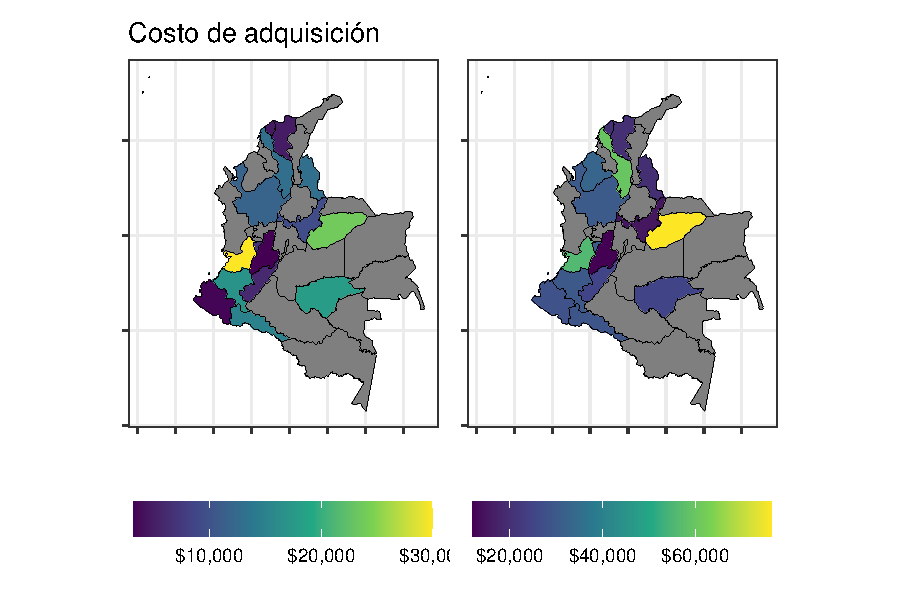
\includegraphics[width=0.9\linewidth]{InformeFinal_files/figure-latex/costoRecetario-1} 

}

\caption{Comparativo de costo vs precio de recetarios por departamento. (A) Costos de adquisición de recetarios por departamento. (B) Precios de recetarios por departamento.}\label{fig:costoRecetario}
\end{figure}

Por otro lado, el precio de venta de los recetarios tiende a rondar los 30.000 COP, ya que en algunos FRE por acto administrativo se ha establecido la tarifa del recetario con base en el salario mínimo diario legal vigente (Figura \ref{fig:costoRecetario}B) que se ajusta cada año. Así mismo, se observa correlación entre los departamentos con costo de recetario más alto y precio de venta mayor, como se da en Valle del Cauca, Bolívar y Casanare.

Ahora bien, el margen de ganancias que deja la venta de recetarios se observa en la Figura \ref{fig:comparativoDepartamentos0}, en donde se puede establecer que con mayor frecuencia los entes territoriales obtienen entre 100 y 200\% de ganancia sobre el costo del recetario. No obstante, los FRE de La Guajira y Nariño, poseen ganancias entre 800 y 900\% en la venta de sus recetarios oficiales. En los FRE de Córdoba, Vichada y Guainía no se registran márgenes de ganancia para la venta de recetarios oficiales dado que no se tiene conocimiento en dichos territorios del costo de adquisición de recetarios puesto que son los entes gubernamentales del departamento los encargados de la contratación, proceso en el que el ente territorial no interviene.

\begin{figure}

{\centering 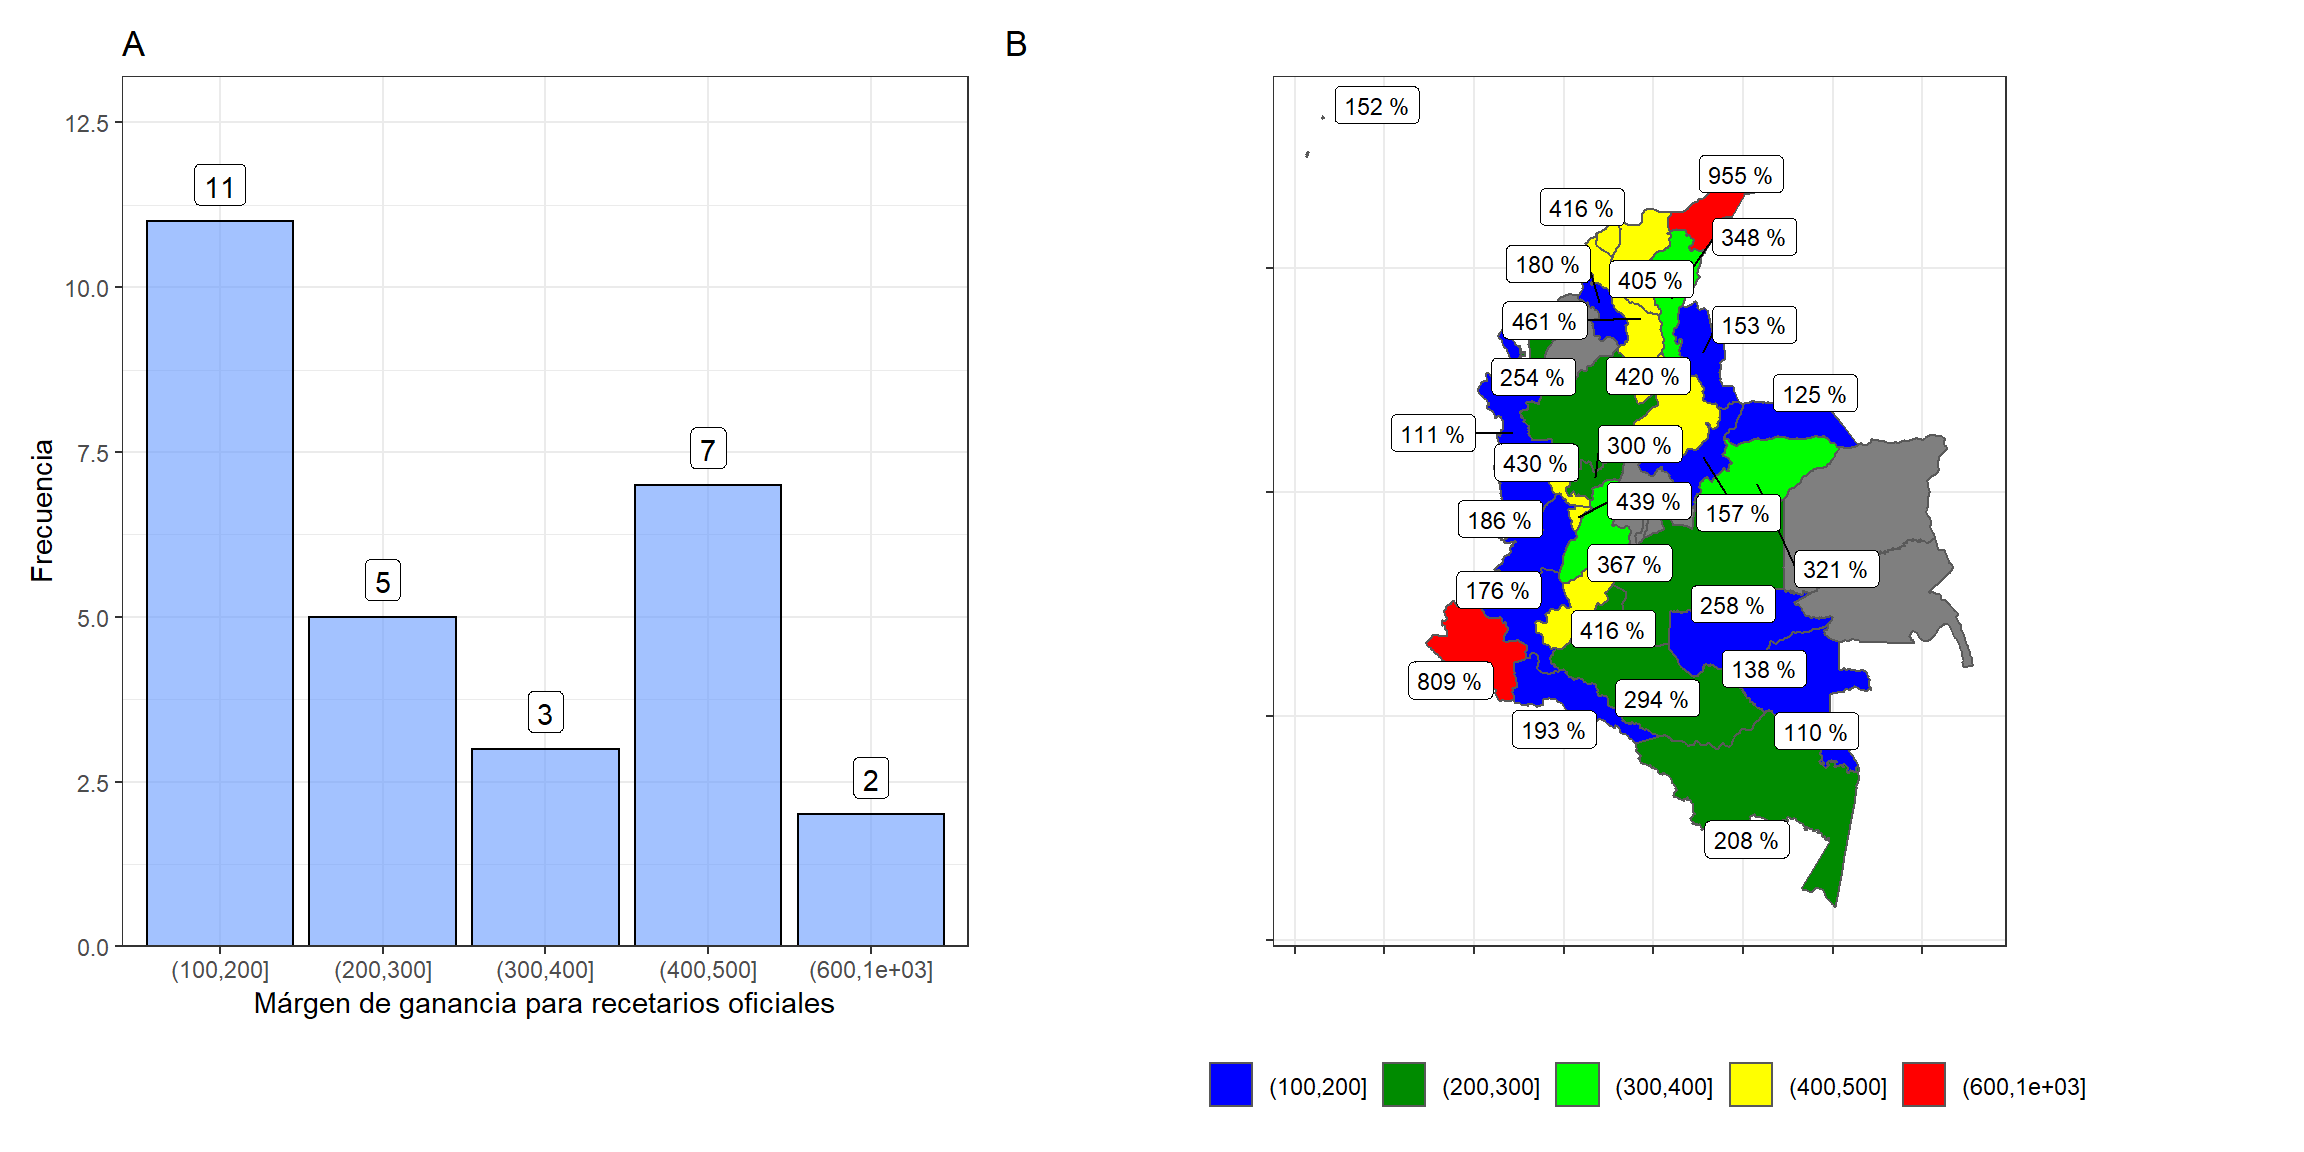
\includegraphics[width=1\linewidth]{InformeFinal_files/figure-latex/comparativoDepartamentos0-1} 

}

\caption{Márgen de ganancia por recetario. (A) Frecuencia de departamentos por márgen de ganancia. (B) Márgen de ganancia de recetarios por departamento.}\label{fig:comparativoDepartamentos0}
\end{figure}

Los amplios márgenes de ganancia y las proporciones distintas entre unos FRE y otros, se podrían relacionar con: (a) cantidad de medidas de seguridad del recetario, (b) facilidad de acceso del departamento, (c) número de prescripciones, (d) tipo de licitación o (e) cantidad de empresas oferentes en los concursos de licitación de recetarios.

\hypertarget{factores-que-afectan-el-costo-de-adquisiciuxf3n-de-recetarios}{%
\subsection{Factores que afectan el costo de adquisición de recetarios}\label{factores-que-afectan-el-costo-de-adquisiciuxf3n-de-recetarios}}

Dentro de los procesos que se utilizan para la licitación y contratación de recetarios oficiales en el país, se consideran 4 modalidades de selección principalmente:

\begin{itemize}
\item
  Licitación pública, el cual es un proceso de selección utilizado por las entidades estatales mediante el cual escoge a sus contratistas a través de una invitación de carácter público que se dirige a todas las personas potencialmente interesadas en ejecutar un contrato, para que en igualdad de condiciones y bajo criterios objetivos garantizados por el pliego de condiciones, presenten ofertas entre las que se escogerá la más favorable\textsuperscript{\protect\hyperlink{ref-MinisteriodeRelacionesExteriores2014}{9}}.
\item
  Selección abreviada, modalidad de selección objetiva prevista en aquellos casos en que por las características del objeto a contratar, las circunstancias de la contratación o la cuantía o destinación del bien, obra o servicio, puedan adelantarse procesos simplificados (uso de subastas a la inversa, bolsas de productos o compras por catálogo) para garantizar la eficacia de la gestión contractual\textsuperscript{\protect\hyperlink{ref-MinisteriodeRelacionesExteriores2014}{9}}.
\item
  Contratación directa, que es de carácter excepcional, por lo que su aplicación es de carácter restrictivo. En efecto, la ley de Contratación Pública en Colombia, prevé los siguientes eventos en los cuales es procedente esta modalidad de contratación: casos de urgencia manifiesta, contratación de empréstitos, cuando no exista pluralidad de oferentes en el mercado, para los contratos de desarrollo de actividades científicas y tecnológicas, entre otros\textsuperscript{\protect\hyperlink{ref-MinisteriodeRelacionesExteriores2014}{9}}.
\item
  Mínima cuantía, que es un procedimiento sencillo y rápido para escoger al contratista en la adquisición de los bienes, obras y servicios cuyo valor no exceda el diez por ciento (10\%) de la menor cuantía de las Entidades Estatales, modalidad de selección que tiene menos formalidades que las demás\textsuperscript{\protect\hyperlink{ref-ColombiaCompraEficiente2019}{10}}.
\end{itemize}

Se realizó una exploración de los factores que pueden afectar el costo de los recetarios mediante un análisis de regresión lineal múltiple, para lo cual se tomó el costo de los recetarios como variable dependiente, y se tuvieron las siguientes variables como variable independientes (regresores):

\begin{itemize}
\item
  número de prescripciones en el recetario (variable continua).
\item
  número de medidas de seguridad implementadas en el recetario (variable continua).
\item
  modalidad de selección de oferentes en la contratación (variable categórica con cuatro niveles mencionadas previamente)
\end{itemize}

\begin{table}

\caption{\label{tab:resumenModeloRegresionLineal}Resumen de modelo de regresión lineal múltiple para el costo del recetario.}
\centering
\begin{tabular}[t]{lcccc}
\toprule
Parámetro & Estimado & Error Estándar & Valor t & Pr(>|t|)\\
\midrule
Intercepto & 12181.9 & 12799.4 & 0.952 & 0.352\\
N.° de prescripciones & 228.1 & 177.8 & 1.283 & 0.213\\
N.° de medidas & -1712.0 & 1578.6 & -1.085 & 0.290\\
Modalidad - Licitación pública & -4760.7 & 12064.4 & -0.395 & 0.697\\
Modalidad - Mínima Cuantía & -3656.2 & 8269.9 & -0.442 & 0.663\\
\addlinespace
Modalidad - Selección abreviada & -1414.0 & 14418.9 & -0.098 & 0.923\\
\bottomrule
\end{tabular}
\end{table}

En la Tabla \ref{tab:resumenModeloRegresionLineal} se muestran los resultados de la regresión lineal múltiple, la modalidad de selección se incluyeron como variables comodín (\emph{dummies}) teniendo en cuenta como referencia a la contratación directa. El modelo generado presenta una bondad de ajuste baja (\(R^{2} = -0.064\)), y no se logra demostrar un efecto significativo de los factores explorados, pese a esto se presentan tendencias en estos factores.

En la Figura \ref{fig:DependParcial1} se muestran gráficos de dependencia parcial de los factores explorados, se observan tendencias como que el N.° de prescripciones elevan el costo de los recetarios. Pese a que se podría suponer que al aumentar el número de características de seguridad en el recetario se aumentaría el costo de este, se encuentra una relación inversa entre el número de medidas y el costo de adquisición. Esto podría deberse a la facilidad de elaboración en departamentos con la capacidad tecnológica adecuada, la forma en que se adjudican los contratos y los diferentes oferentes en el concurso de contratación.

\begin{figure}

{\centering 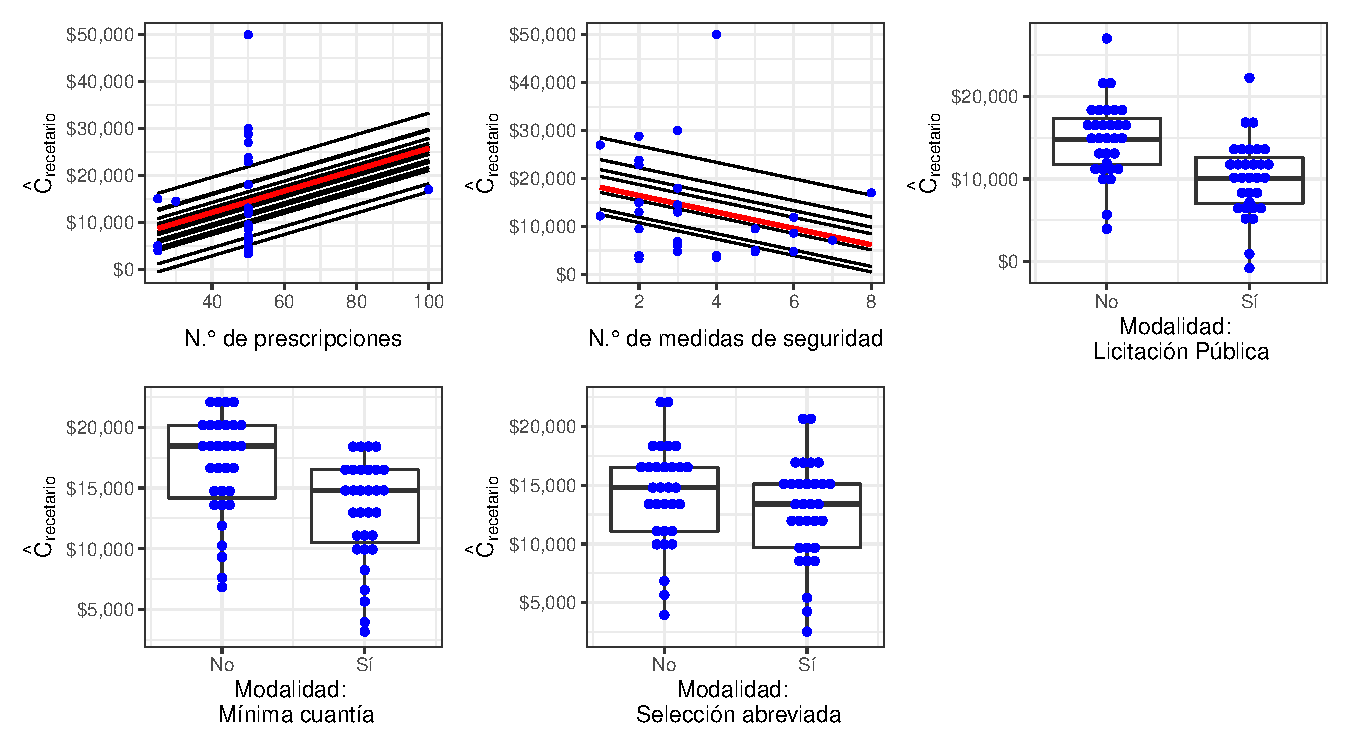
\includegraphics[width=0.9\linewidth]{InformeFinal_files/figure-latex/DependParcial1-1} 

}

\caption{Gráficos de dependencia parcial - Modelo de costos de recetarios.}\label{fig:DependParcial1}
\end{figure}

De esta forma, el tipo de contratación que se concreta con las empresas fabricante de los recetarios es una variable que influye en el costo de los recetarios, así pues, las modalidades de contratación por licitación pública, mínima cuantía y selección abreviada tienden a disminuir el costo del recetario en comparación con la modalidad de contratación directa, factor esperado ya que al no haber competencia entre empresas oferentes, quien posee el monopolio de fabricación es libre de disponer los precios de venta a las entidades territoriales.

Por otra parte, los FRE que concretaron órdenes de compra de recetarios por mínima cuantía y selección abreviada, tienden a presentar precios mayores de adquisición, con costo alrededor de los 10.000 COP y 15.000 COP, mientras que, los entes territoriales que optaron por la modalidad de licitación pública tienden a ser los recetarios más económicos en relación con las demás, con costos inferiores a los 10.000 COP por recetario en promedio.

\hypertarget{precio-de-venta-de-recetario-por-prescripciuxf3n}{%
\subsection{Precio de venta de recetario por prescripción}\label{precio-de-venta-de-recetario-por-prescripciuxf3n}}

Finalmente, se concluye que el precio por prescripción de los recetarios oficiales circulantes a nivel nacional como variante ponderadora el precio de venta y la cantidad de prescripciones por recetario, en donde se puede evidenciar la tendencia de los FRE hacia 250 COP a 500 COP por prescripción (Figura \ref{fig:PVTA-Recetarios}).

\begin{figure}

{\centering 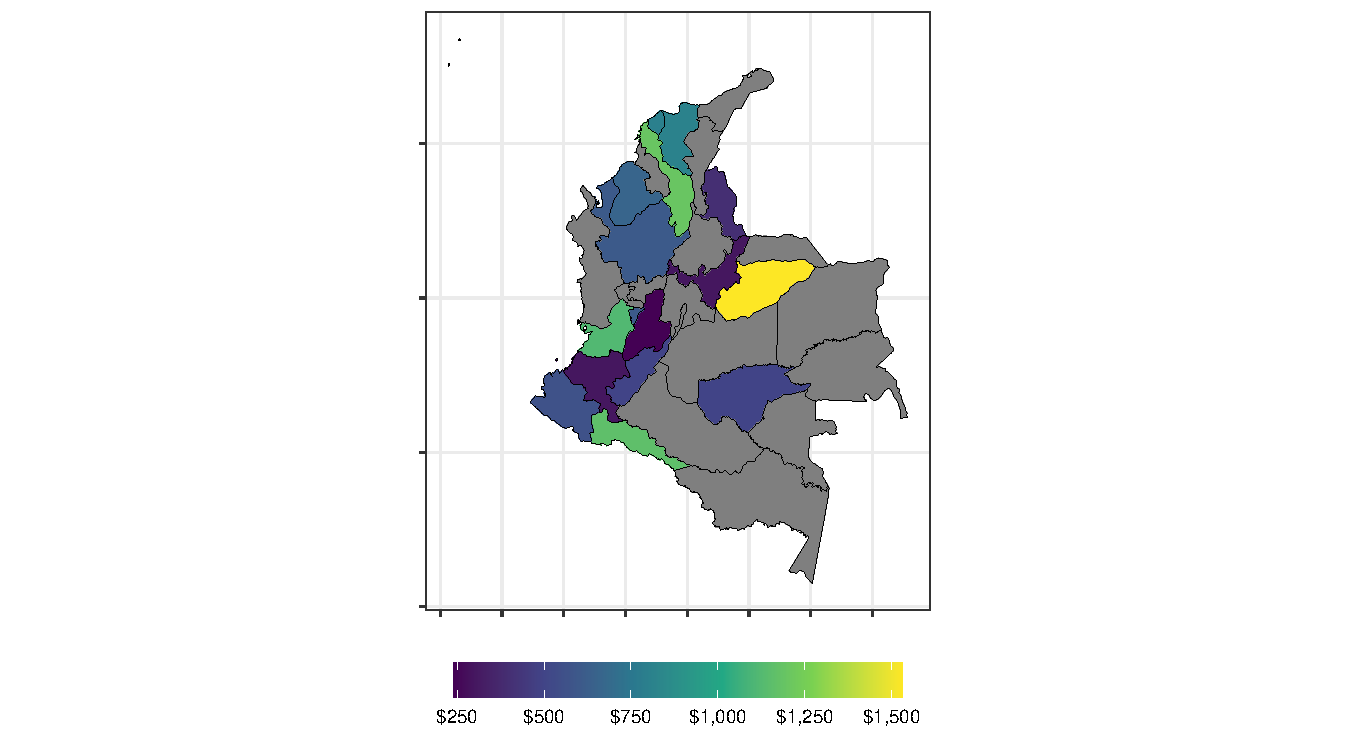
\includegraphics[width=0.9\linewidth]{InformeFinal_files/figure-latex/PVTA-Recetarios-1} 

}

\caption{Precio de venta de recetario por prescripción.}\label{fig:PVTA-Recetarios}
\end{figure}

El valor por prescripción más alto a nivel nacional se presenta en el departamento de Casanare, pese a que este recetario cuenta con 50 prescripciones como la mayoría de los FRE, su precio de venta es de 76.500 COP, el más alto del país, y del que no se tiene un acto administrativo donde se establezca su valor. Además de ello, cuenta con 3 medidas de seguridad, lo que consolida la hipótesis que se observa a nivel nacional que indica que, a menor número de medidas de seguridad, mayor es el costo del recetario.

El precio de venta por prescripción podría incrementar los costos a los que se venden los MME a los pacientes en los puntos de dispensación.

\hypertarget{adquisiciuxf3n-de-recetarios}{%
\section{Adquisición de recetarios}\label{adquisiciuxf3n-de-recetarios}}

\maxdeadcycles=1000

\hypertarget{proceso-de-adquisiciuxf3n-de-recetario}{%
\subsection{Proceso de adquisición de recetario}\label{proceso-de-adquisiciuxf3n-de-recetario}}

La adquisición de recetarios oficiales por parte de los FRE es un proceso que se lleva a cabe mediante contratación pública. En la Figura \ref{fig:modalidadAdquisicion}, se muestra un resumen de las modalidades de selección en el último proceso de adquisición de recetarios por parte de los FRE. Se evidencia que la modalidad más utilizada en este último periodo de reabastecimiento de recetario fue mínima cuantía.

\begin{figure}

{\centering 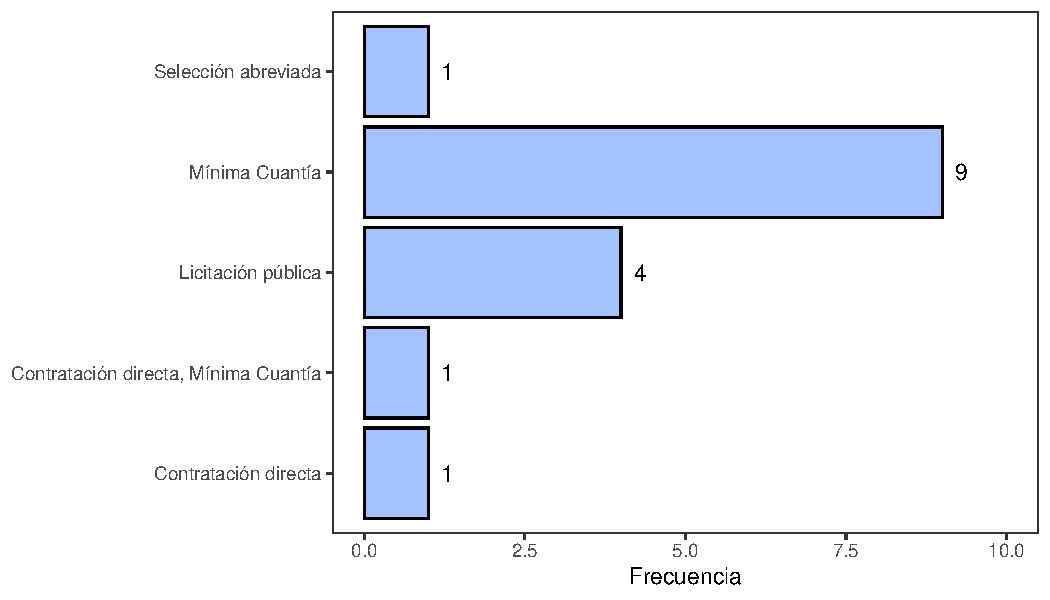
\includegraphics[width=0.85\linewidth]{InformeFinal_files/figure-latex/modalidadAdquisicion-1} 

}

\caption{Modalidad de selección para contratos de adquisición de recetarios.}\label{fig:modalidadAdquisicion}
\end{figure}

De acuerdo con los entes territoriales, esta modalidad de selección presenta favorabilidad desde el punto de vista financiero respecto a la inversión y recaudo posterior tras la venta de los recetarios oficiales. El ingreso por venta de recetarios es una de las principales fuentes de financiación de varios FRE (ver Figura \ref{fig:IngresosFRE1}).

La selección por mínima cuantía tiene como desventaja que algunos requerimientos funcionales del objeto a contratar pueden ser pasados por alto, y esto puede poner en riesgo el cumplimiento de las especificaciones del usuario en cuanto a los recetarios recibidos. De hecho, se observaron ejemplos donde debido a la falta de: (i) verificación de la experiencia del proponente, (ii) seguimiento y/o (iii) auditoria del avance de entrega, se recibieron recetarios no conformes, con prescripciones sin codificación o tintas desgastadas.

La segunda modalidad de selección más frecuente fue licitación pública, en la cual se exige demostrar tiempo de experiencia relacionada a la elaboración de este tipo de insumos. Por ejemplo, sí el recetario cuenta con medidas de seguridad específica (ver Figura \ref{fig:MedidasSeguridad-Almacenamiento}) se espera que el proponente logre demostrar la capacidad de cumplir con la entrega del producto especificado.

Los departamentos con mayor número de características de seguridad en el recetario oficial suelen realizar la contratación mediante licitación pública. Esta modalidad de selección podría favorecer la calidad del producto recibido y esto podría evitar problemas por falsificación del recetario. Sin embargo, en varios departamentos se podrían tener problemas para implementar esta modalidad debido a la falta de oferentes.

Entre las medidas de seguridad más observadas en los recetarios por licitación pública se encuentran el uso de tintas invisibles o fluorescentes en secciones específicas del recetario que brillan bajo la luz UV, bandas y/o filamentos de seguridad, versus las medidas de seguridad de recetarios realizados por mínima cuantía como seriales con codificaciones alfanuméricas, escudo de la gobernación respectiva y/o marcas de agua.

Pese a que la modalidad de selección en los contratos de adquisición de recetarios es un factor que afecta de forma importante el costo, se debe tener en cuenta que en algunos departamentos existe un rubro dentro de la gobernación para papelería y de este mismo se compran los recetarios, sin tener conocimiento del valor destinado para estos insumos por parte del FRE.

En el marco de las actividades de las Jornadas de inmersión territorial, se logró observar un patrón en el proceso de licitación y contratación de recetarios oficiales por los FRE alrededor del país. Como se evidencia en la Figura \ref{fig:procesoContractual}, en la mayoría de los casos, los funcionarios de los FRE se encargan exclusivamente de la realización de los estudios previos, en donde se solicita la necesidad en cantidad y forma de recetarios. Posterior a ello, es la dirección territorial en salud, que en algunos casos es la secretaria de salud departamental, la gobernación u otra dependencia con interés en la salud pública del territorio, la encargada de desarrollar la etapa contractual del proceso, mediante una de las modalidades de selección de oferentes que más convenga, se elige la empresa proveedora y se establece el contrato de elaboración de recetarios oficiales.

\begin{figure}

{\centering 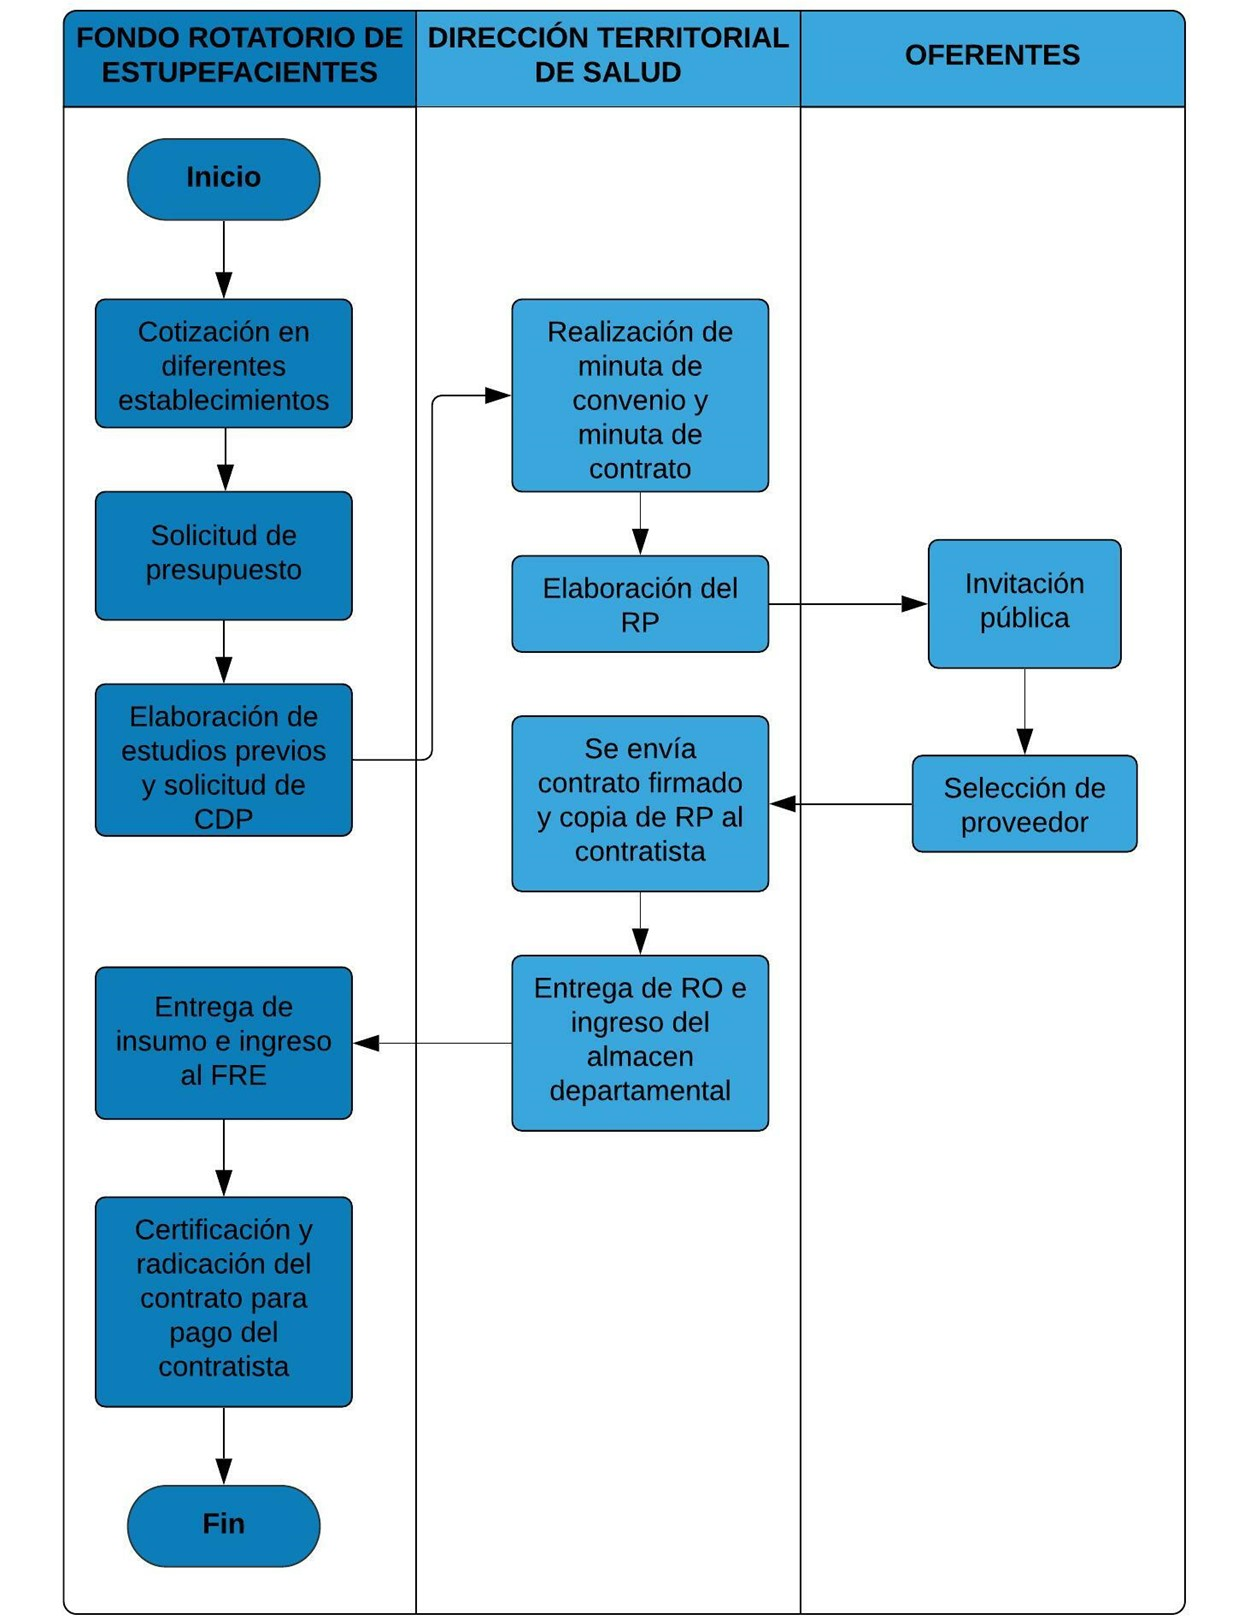
\includegraphics[width=0.8\linewidth]{figures/procesoContractual} 

}

\caption{Proceso de contratación/licitación de los recetarios oficiales.}\label{fig:procesoContractual}
\end{figure}

\hypertarget{tiempos-de-adquisiciuxf3n}{%
\subsection{Tiempos de adquisición}\label{tiempos-de-adquisiciuxf3n}}

\begin{figure}

{\centering 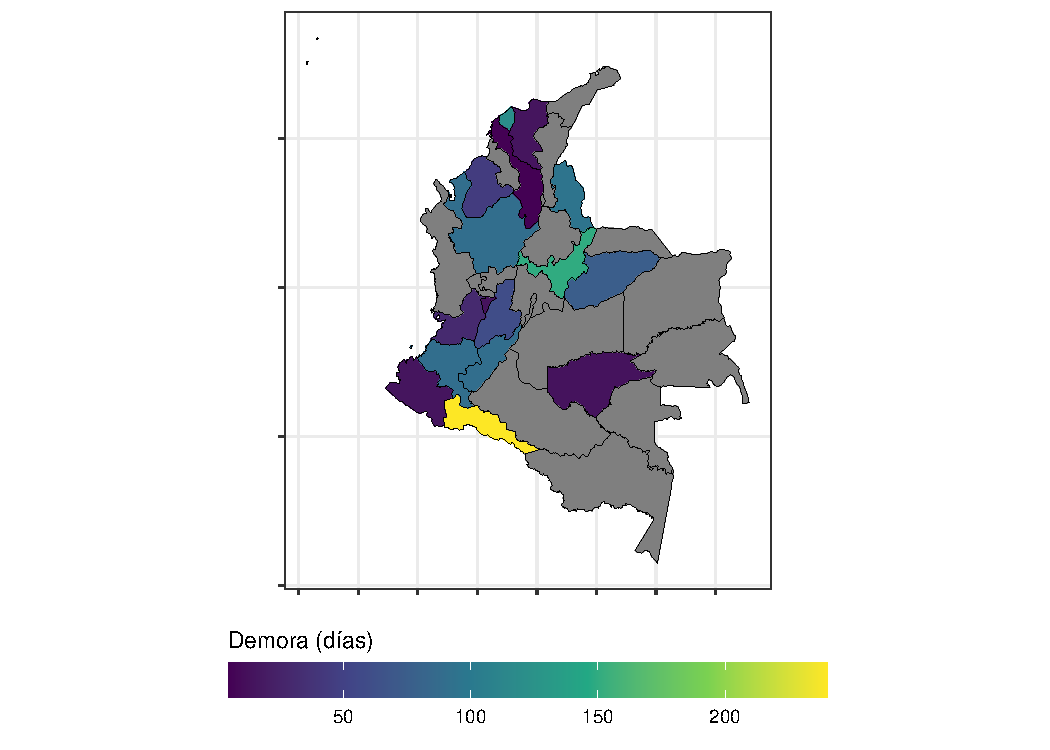
\includegraphics[width=0.85\linewidth]{InformeFinal_files/figure-latex/tiempoDemoraAdquisicion-1} 

}

\caption{Tiempo de demora para adquisición de recetarios.}\label{fig:tiempoDemoraAdquisicion}
\end{figure}

En la Figura \ref{fig:tiempoDemoraAdquisicion} se muestra el tiempo promedio que toma el proceso de adquisición de recetarios oficiales por parte de los entes territoriales, se evidencia que el tiempo promedio se encuentra entre 60 y 120 días (2 a 4 meses).

Por otro lado, se observó que los departamentos que compran los recetarios por la modalidad de contratación directa son aquellos con menores tiempos de adquisición, tiempos de aproximadamente 1 mes. Mientras que, los departamentos que compran por medio de mínima cuantía y licitación pública tienen mayor variabilidad en el tiempo de adquisición que pueden tardar entre 1 a 8 meses.

La \emph{etapa precontractual} (estudios previos, estudios de mercado y estimación de necesidad) del proceso de adquisición suele ser realizada por el personal del FRE. Estos procesos iniciales toman poco tiempo y suelen tomar entre 1 semana y 2 meses.

Por otra parte, la \emph{etapa contractual} suele ser realizada por la gobernación y puede tardar en completarse de 1 a 2 meses, o en casos particulares más de 2 meses. Estos tiempos estimados en la etapa contractual fueron informados por los FRE, sin embargo, los mismos desconocen el detalle el proceso que se lleva a cabo.

La etapa de despacho de los recetarios puede tomar entre 1 a 3 meses en ejecutarse por parte de los contratistas, y estos tiempos son particulares para cada departamento dependiendo del volumen de recetarios adquiridos y el nivel de especificación acordado, entre otros.

Existen casos atípicos como el FRE del departamento de Putumayo, el cual lleva sin concretar la compra de recetarios oficiales desde el mes de noviembre del año 2020. La principal problemática de adquisición del FRE Putumayo es debida a dificultades de la gobernación con el proceso de licitación.

En algunos departamentos se utiliza la plataforma Colombia Compra Eficiente para la adquisición de recetarios. Se encuentran algunos departamentos que han experimentado dificultades con esta plataforma y esto ha resultado en demoras en el proceso de adquisición de recetarios.

\hypertarget{procesos-relacionados-a-los-recetarios}{%
\section{Procesos relacionados a los recetarios}\label{procesos-relacionados-a-los-recetarios}}

\maxdeadcycles=1000

\hypertarget{recepciuxf3n-de-recetarios}{%
\subsection{Recepción de recetarios}\label{recepciuxf3n-de-recetarios}}

En relación con la Figura \ref{fig:ReciboRecetariosInstituciones}A, se puede observar que 17 de los FRE entrevistados confirmaron que, sí reciben los recetarios diligenciados de las instituciones inscritas en su despacho dentro de los tiempos estimados, ver Figura \ref{fig:ReciboRecetariosInstituciones}B. Esto se realiza con el fin de corroborar los informes allegados correspondientes al anexo 13 que se entregan mensualmente.

\begin{figure}

{\centering 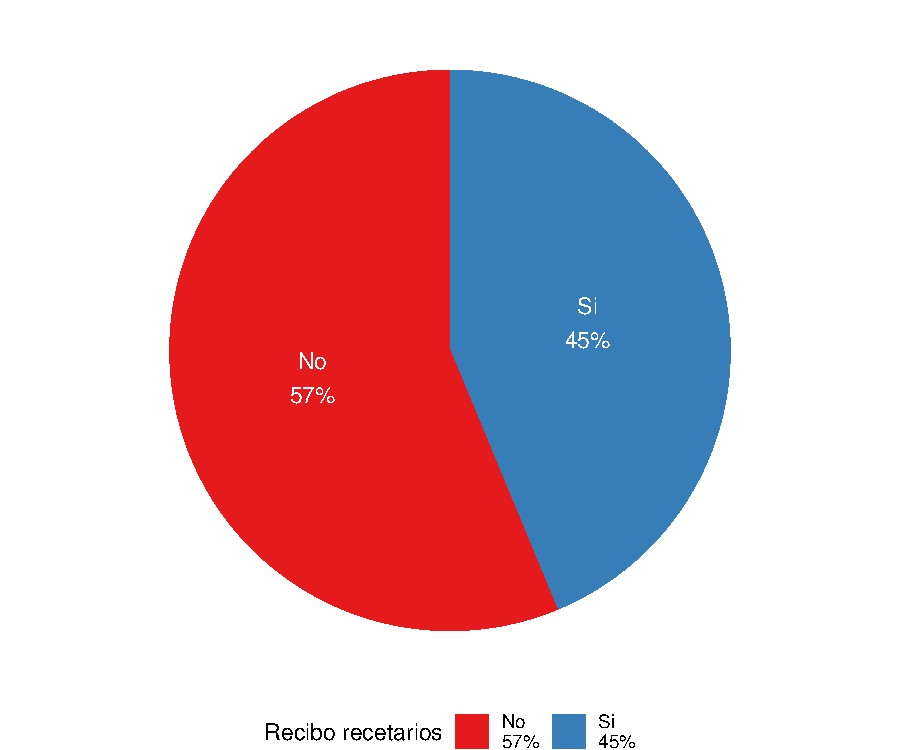
\includegraphics[width=1\linewidth]{InformeFinal_files/figure-latex/ReciboRecetariosInstituciones-1} 

}

\caption{Recepción de recetarios. (A) Porcentaje de entes territoriales que reciben recetarios oficiales recibidos prescritos/diligenciados. (B) Tiempo de recepción de recetarios oficiales desde IPS.}\label{fig:ReciboRecetariosInstituciones}
\end{figure}

Los recetarios entregados deben revisarse exhaustivamente para evidenciar el buen uso de estos. Junto con los recetarios se trae el anexo 13 para corroborar que los medicamentos formulados coincidan con los valores prescritos en cada uno de los mismos. Esta tarea se realiza en 17 de los 31 departamentos visitados, sin embargo, es una actividad demorada debido a la: (a) falta de personal en los entes territoriales y (b) cantidad de instituciones inscritas y/o médicos prescriptores que hay en el departamento.

El resto de los departamentos (57\%) no reciben los recetarios prescritos en físico, entre las razones, la más frecuente está relacionada con la capacidad de almacenamiento del FRE de este tipo de documentación, que suele ser muy limitado o no se cuenta con el mismo. En dichos casos, los FRE han optado por emitir circulares, solicitando a las entidades y médicos prescriptores inscritos que mantengan la custodia de los talonarios diligenciados, como parte de la historia clínica de los pacientes, hasta que el FRE realice la visita de inspección, vigilancia y control. Una vez allí, se realiza un muestreo para verificar que las fórmulas prescritas en un determinado tiempo concuerden con las cantidades de medicamentos reportados en los informes mensuales.

\hypertarget{venta-de-recetarios-oficiales}{%
\subsection{Venta de recetarios oficiales}\label{venta-de-recetarios-oficiales}}

El proceso de venta de recetarios oficiales se lleva a cabo de forma estandarizada en el grueso de los FRE del país, siguiendo el procedimiento descrito en la Figura \ref{fig:procesoVentaRec}. Allí se observa se forma generalizada la primera instancia del proceso, la cual es la solicitud de cotización de recetarios oficiales al FRE. Esta puede ser de forma personal o vía correo electrónico. Posterior a ello, el ente territorial realiza su estudio interno de disponibilidad y responde a la institución interesada con la cantidad que puede vender, de ser el caso en que no disponga del total de recetarios que el establecimiento farmacéutico requirió.

\begin{figure}

{\centering 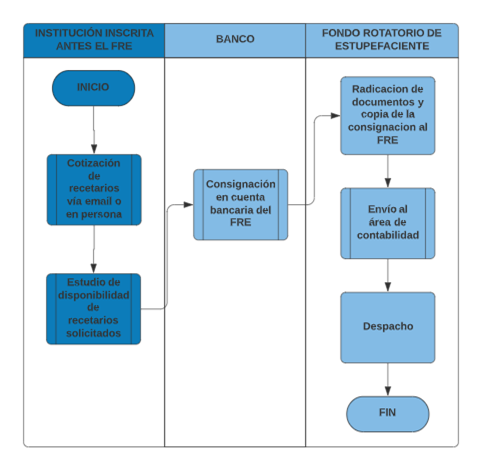
\includegraphics[width=0.8\linewidth]{figures/procesoVentaREC} 

}

\caption{Proceso de venta de recetarios oficiales.}\label{fig:procesoVentaRec}
\end{figure}

Según la Resolución 1479 de 2006\textsuperscript{\protect\hyperlink{ref-MSPS1479-2006}{2}} - articulo 3, cada FRE debe contar con una cuenta bancaria en donde administre sus operaciones. En esta cuenta es donde la institución interesada deposita el monto de la cotización realizada. Finalmente, se radica ante el FRE el soporte de pago y los documentos de la cotización para que sean enviados al área de contabilidad del ente territorial, y los recetarios despachados al establecimiento farmacéutico que los requiere.

Este proceso de venta de recetarios oficiales se desarrolla de forma rápida como lo demuestra la Figura \ref{fig:TiempoVentaInstituciones}. En la mayoría de departamentos tarda entre 1 y 2 días concretar la venta, tiempo que es determinado realmente por el establecimiento y cuanto demore en hacer el pago bancario a la cuenta del FRE. Los casos particulares en que el proceso toma hasta 5 días o más, como es el caso particular del FRE de Norte de Santander, se da por el alto riesgo de desvíos y posibilidad de fraudes de recetarios oficiales, por lo que los funcionarios del ente territorial, se toman una semana para realizar exhaustivamente la revisión del comprador. Por otro lado, en los FRE de Huila, Tolima y Vaupés, este comportamiento se presenta principalmente por falta de personal que pueda abarcar el total de las actividades que debe desarrollar el ente territorial, panorama común dentro de lo observado a lo largo de los acompañamientos técnicos del Proyecto de inversión Misión PRI 1901 a los distintos FRE de la nación, en donde por carencia de personal suficiente se tienen que priorizar unas tareas y relegar otras actividades del ente territorial igualmente valiosas para la salud pública de la región.

\begin{figure}

{\centering 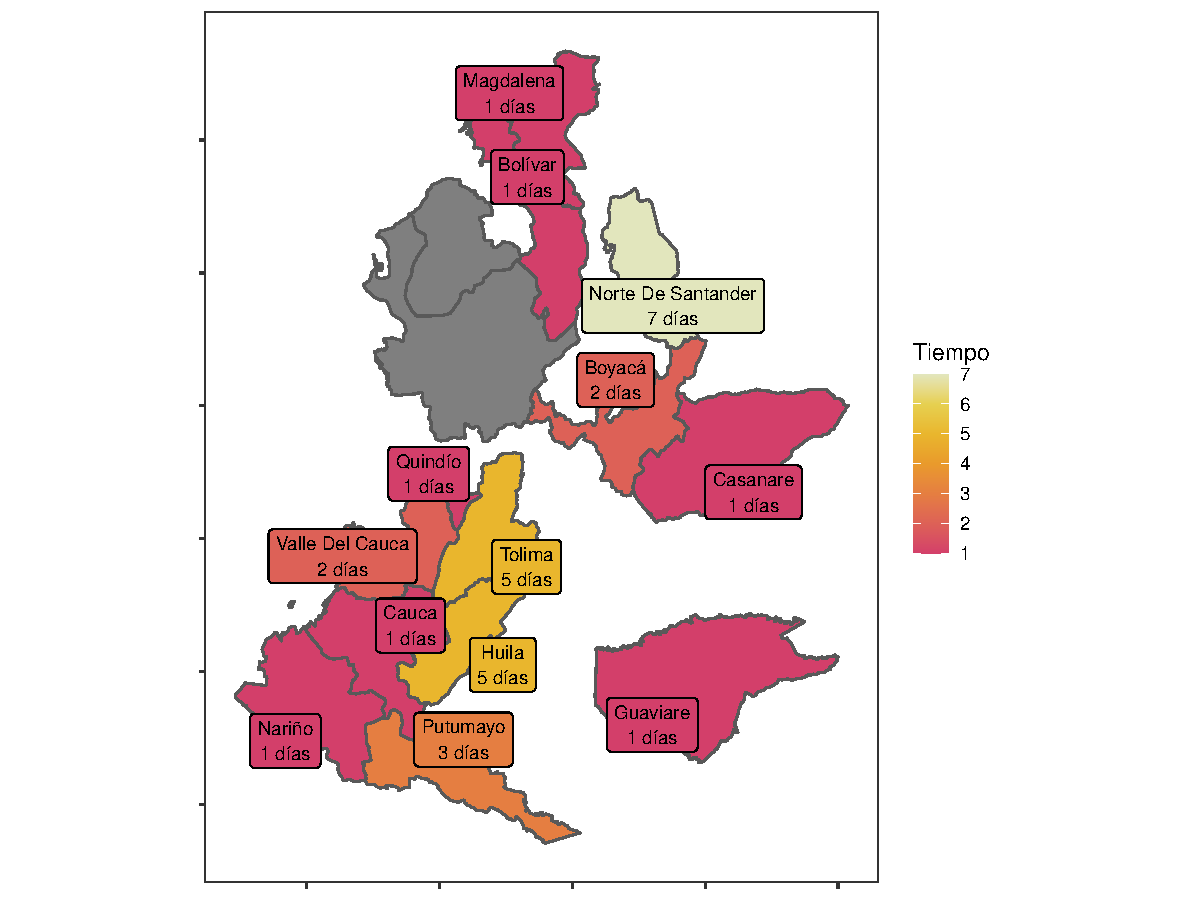
\includegraphics[width=0.9\linewidth]{InformeFinal_files/figure-latex/TiempoVentaInstituciones-1} 

}

\caption{Tiempo de demora en la venta de recetarios oficiales a clientes.}\label{fig:TiempoVentaInstituciones}
\end{figure}

\hypertarget{seguimiento-a-uso-de-recetarios}{%
\subsection{Seguimiento a uso de recetarios}\label{seguimiento-a-uso-de-recetarios}}

La Figura \ref{fig:BD-diligBDRecet} muestra los campos de información recolectada en bases de datos por los FRE al momento de realizar la venta de un recetario oficial, la información recolectada permite conocer entre otras cosas:

\begin{itemize}
\item
  Datos básicos de las entidades y prescriptores inscritos en el FRE.
\item
  Unidades consumidas y su respectivo valor.
\item
  Datos de identificación de los recetarios.
\item
  Número de talonarios que se distribuyen en los respectivos departamentos.
\end{itemize}

\begin{figure}

{\centering 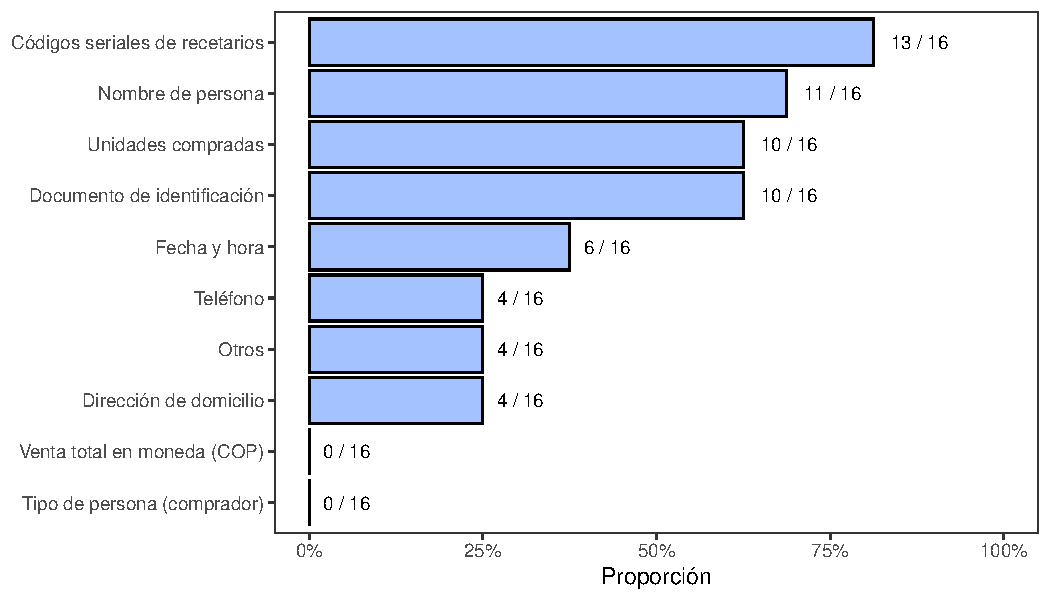
\includegraphics[width=0.85\linewidth]{InformeFinal_files/figure-latex/BD-diligBDRecet-1} 

}

\caption{Proporción de FRE que diligencian campos en BD de venta de recetarios}\label{fig:BD-diligBDRecet}
\end{figure}

Durante la jornada de inmersión territorial, se puedo observar que los FRE utilizan dichas bases con dos propósitos principales:

\begin{itemize}
\item
  Realizar estimaciones de necesidad de recetarios, control de inventarios y control en las cantidades que los compradores adquieren. Esto permite llevar un seguimiento del consumo promedio de las entidades. Este control permitió a los FRE realizar un seguimiento a posibles desvíos o anormalidades en los consumos. Por ejemplo, con el inicio de la pandemia el consumo de ROs y MME aumentó en la mayoría de los departamentos, por lo que los FRE tuvieron que fortalecer el trabajo en equipo con las entidades para mitigar desabastecimientos.
\item
  Evitar fraudes o falsificaciones al realizar un control en el manejo de talonarios, y contrastando la información de las bases con la entregada o solicitada durante visitas.
\end{itemize}

Se observó que la mayoría de FRE (proporción mayor a 50\% en la Figura \ref{fig:BD-diligBDRecet}) llevaban un control de información con el fin de identificar a los compradores (Nombre del comprador persona o institución) y las cantidades adquiridas -- Unidades compradas. Se almacenan datos de contacto, como dirección o teléfono en tan solo 25\% de los FRE. Por otro lado, se evidenció que la mayoría de departamentos (83\%) optan por realizar seguimiento a los recetarios con el código de serial, debido a que estos son únicos en cada recetario.

Así mismo, se observaron otros tipos de campos almacenados por los FRE (opción Otros) en la venta de recetarios. Entre estos otros se encuentra: (a) consecutivos de las facturas emitidas en cada compra, (b) registro REPS, (c) saldo de recetarios oficiales tras la compra, o (d) códigos de recetarios oficiales prescritos allegados para su revisión. Algunos FRE cierran el ciclo de control del RO, en la misma base de datos, al relacionar los RO prescritos que son devueltos para su revisión.

Los FRE realizan una serie de actividades para el seguimiento de uso de los recetarios. En la Figura \ref{fig:SeguimientoUsoRecetarios} se muestra las distintas acciones realizadas por parte de los FRE para el seguimiento al manejo de los RO. La actividad de control más realizada, alrededor de un 70\%, es la visita a las instituciones y médicos independientes inscritos en el FRE. La dinámica principal de la visita consiste en actividades propias de IVC, y a su vez en la revisión del anexo 13 junto con otros informes particulares vs las copias de las prescripciones de los RO que las entidades tengan disponibles.

Las visitas a instituciones han permitido evidenciar en algunos departamentos, falencias en el uso adecuado de los RO, como por ejemplo prescripciones en las cuales se formulan antibióticos u otros medicamentos en conjunto con MME o solos, así mismo se tienen casos donde se encuentran recetarios en blanco, pero con firma y sello del médico prescriptor, generando un alto riesgo de desvío en las instituciones.

En segundo lugar, se encuentra la verificación de base de ventas. Esta actividad se explicó al mencionar que las mismas se utilizan para el control y seguimiento de posibles desvíos o anormalidades en los consumos.

Las actividades anteriormente descritas se consideran actividades de seguimiento pasivas, caso contrario a la verificación de recambios. Esta actividad se realiza en un 22\% del territorio Nacional, la cual consiste en autorizar la venta de recetarios a las entidades y/o médicos prescriptores solo sí devuelve los recetarios comprados anteriormente. Por parte de los departamentos se aclara que no es necesarios vender la misma cantidad de recetarios que el comprador devuelve.

Otras actividades de seguimiento activo al manejo de RO son el seguimiento a las denuncias, las cuales tienen una proporción menor al 5\%. Finalmente, el acompañamiento permitió evidenciar que el 15\% de los FRE no realizan ningún tipo de actividad de seguimiento al uso de los ROs, tan solo cumpliendo con la presentación de informes exigidos por la normativa vigente.

\begin{figure}

{\centering 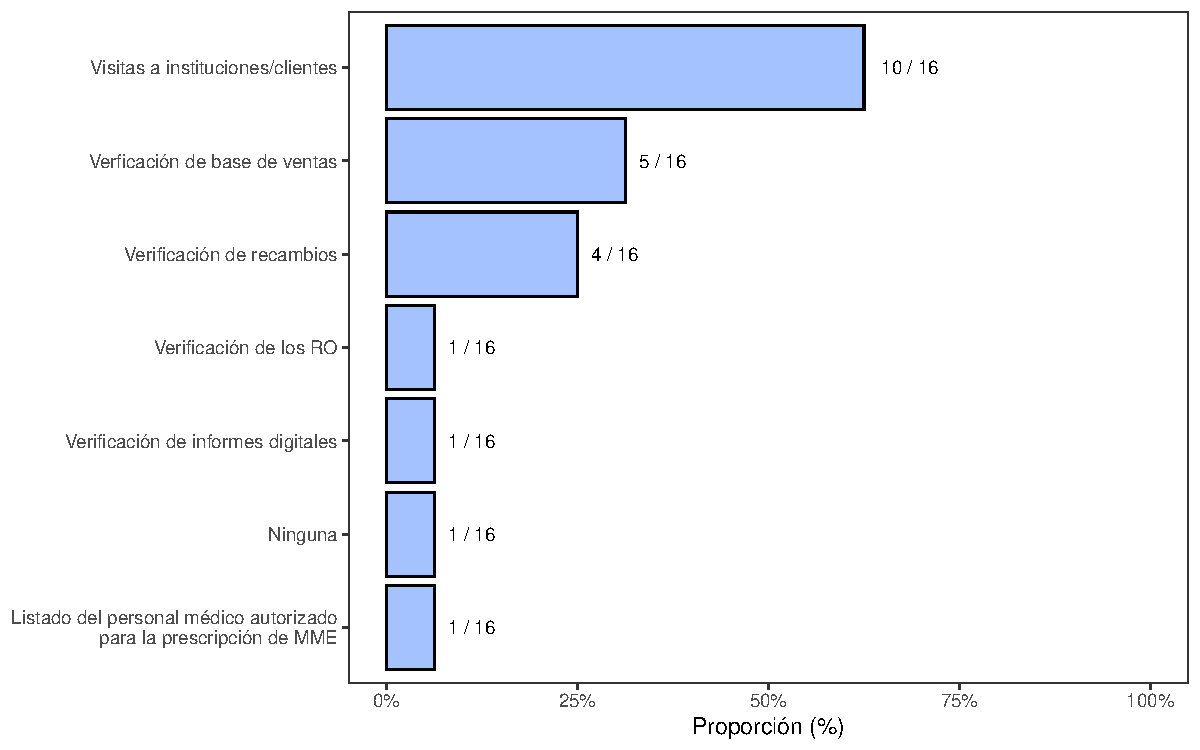
\includegraphics[width=0.85\linewidth]{InformeFinal_files/figure-latex/SeguimientoUsoRecetarios-1} 

}

\caption{Actividades realizadas por el FRE para el seguimiento del uso de recetarios.}\label{fig:SeguimientoUsoRecetarios}
\end{figure}

\hypertarget{archivo-de-recetarios}{%
\subsection{Archivo de recetarios}\label{archivo-de-recetarios}}

Durante el acompañamiento se complementó como recomendación a los FRE, se considerará alinearse a lo expresado en la Circular 009 de 2015 del FNE, donde se difunde la buena práctica de implementar bases de retención documental y gestión de archivo\textsuperscript{\protect\hyperlink{ref-FNE2015-9}{11}}. La frecuencia con la cual se reciben los recetarios oficiales a los FRE desde las entidades y médicos prescriptores inscritos se observa en la Figura \ref{fig:ReciboRecetariosInstituciones}B La frecuencia de recepción de recetarios guarda relación con la información analizada en el punto anterior. Se tiene que 13 FRE reciben los 10 primeros días del mes los recetarios oficiales prescritos conforme a lo solicitado a las instituciones de cada departamento, mientras que los otros 4 FRE no han estandarizado el tiempo de entrega y reciben los recetarios oficiales a lo largo del mes, asegurando su recepción mediante recordatorio por correo electrónico o comunicación telefónica, si llega a ser requerido. Se tiene que 17 de 31 FRE reciben los recetarios oficiales desde IPS.

Complementando la información reportada en la Figura \ref{fig:ReciboRecetariosInstituciones} y en la Figura \ref{fig:TiempoArchivoRecetariosOficiales}, se relacionó el tiempo de archivo que los FRE que si reciben los recetarios oficiales los almacenan, obteniendo que 10 FRE los almacenan por un periodo mayor a 5 años. Durante las jornadas de inmersión territorial se pudo observar que este tiempo de almacenamiento, en la mayoría de los casos, es por desinformación en los FRE, puesto que no se tiene presente el tiempo que se deben guardar estas copias, y al considerarlas parte de la historia clínica de un paciente estiman guardarlas hasta por 10 años, superando en muchos casos la capacidad de archivo de los FRE.

\begin{figure}

{\centering 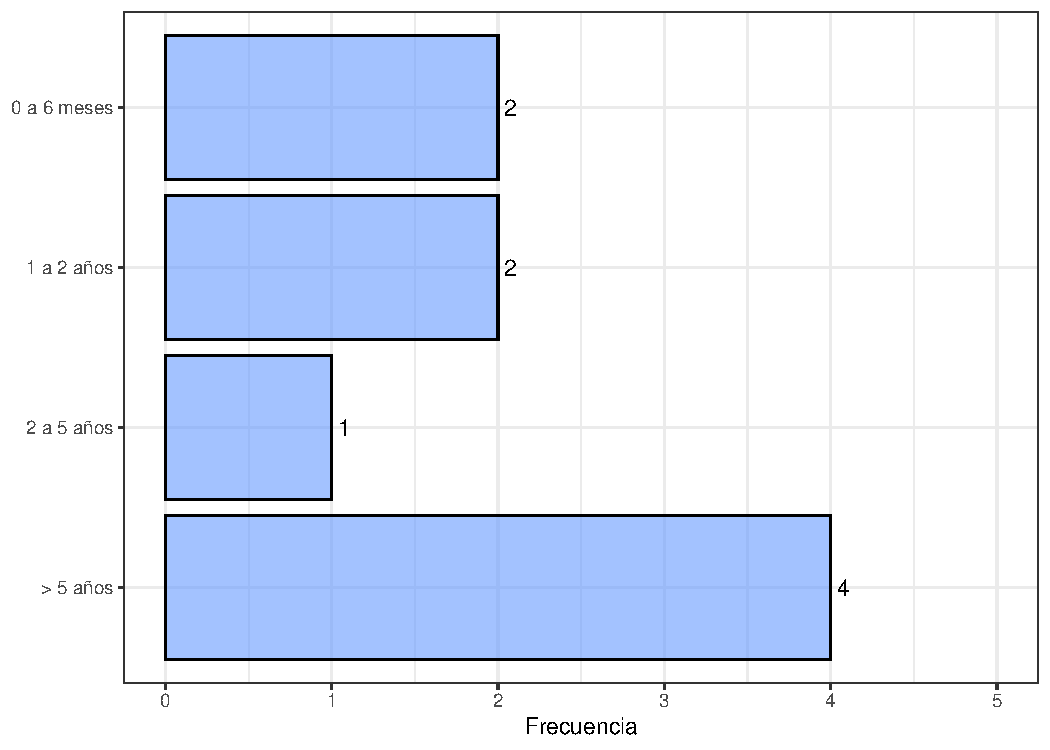
\includegraphics[width=0.85\linewidth]{InformeFinal_files/figure-latex/TiempoArchivoRecetariosOficiales-1} 

}

\caption{Tiempo de archivo de los recetarios oficiales en los FRE.}\label{fig:TiempoArchivoRecetariosOficiales}
\end{figure}

En otros casos, la intención de archivo se acoge a las medidas establecidas por las gobernaciones, en las cuales se pide un archivo de 20 años para documentación critica, según las tablas de retención documental gubernamental\textsuperscript{\protect\hyperlink{ref-PresidenciadelaRepublicadeColombia2012}{12}}. Otros FRE en cambio establecieron protocolo de archivo y una vez cumplido el periodo de almacenamiento, por supuesto, posterior revisión, los recetarios oficiales son destruidos.

Como se mencionó previamente durante el acompañamiento se compartió la Circular 009 de 2015\textsuperscript{\protect\hyperlink{ref-FNE2015-9}{11}}, la cual en su Artículo Primero expresa:

\begin{quote}
\emph{``Que las autoridades administrativas, los fabricantes, los comerciantes, los hombres de ciencia, las Instituciones científicas y los hospitales lleven registros en que consten las cantidades de cada estupefaciente fabricado, y de cada adquisición y destino dado a los estupefacientes. Dichos registros serán conservados por un periodo de dos años por lo menos. Cuando se utilicen talonarios (artículo 30, inciso 2 b) de recetas oficiales, dichos talonarios se conservarán también durante un periodo de dos años por lo menos''.}
\end{quote}

En este sentido, los FRE buscarán adoptar dicha medida para liberar espacio de almacenamiento, con el fin de que pueda ser aprovechado para otro tipo de insumos.

Debido a que los recetarios oficiales son el requisito obligatorio para la dispensación de medicamentos de control especial o monopolio del estado, se ha visto la necesidad de resguardar los talonarios en áreas seguras y de acceso limitado para evitar robos o desvíos. En la Figura \ref{fig:MedidasSeguridad-Almacenamiento} se observa que todos los departamentos han implementado algún tipo de medida de seguridad para el control de los recetarios.

\begin{figure}

{\centering 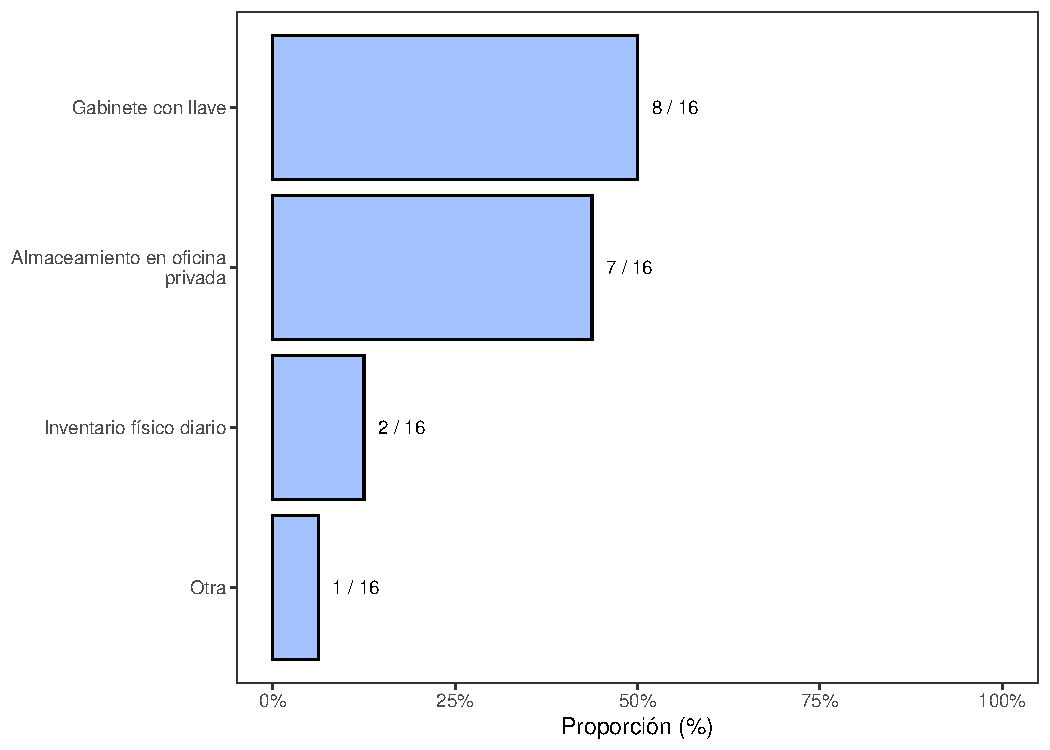
\includegraphics[width=0.85\linewidth]{InformeFinal_files/figure-latex/MedidasSeguridad-Almacenamiento-1} 

}

\caption{Proporción de FRE con medidas de seguridad implementada en almacenamiento de recetarios.}\label{fig:MedidasSeguridad-Almacenamiento}
\end{figure}

La mayoría de los FRE, más del 70\%, han optado por almacenar los recetarios oficiales en gabinetes u oficinas privadas con acceso limitado al personal del FRE, con el objetivo de garantizar la custodia de los mismos y evitar pérdidas, de preferencia en espacios que además aseguren su buen estado físico. Hasta el momento, estas medidas de seguridad han sido suficientes puesto que durante el acompañamiento no se encontraron casos en los cuales los FRE hayan mencionado históricos de situaciones de robo o pérdida de recetarios. Sin embargo, durante el proyecto de inversión, especialmente durante las visitas a las que se tuvo acceso presencial o imágenes de las oficinas de almacenamiento, se pudo evidenciar que, si bien los recetarios están almacenados en oficinas privadas o gabinetes con llave, las condiciones para tal fin no son las adecuadas, se tienen situaciones donde se comparten espacios con los medicamentos, y dichos espacios no son suficientes, por lo que se deben disponer en lugares estrechos de las oficinas del FRE.

Adicionalmente, los FRE suelen solicitar mejoras en la infraestructura o seguridad de las oficinas, pero la inversión se ve limitada por autorización y/o estudio de recursos económicos para estos proyectos financiada en la mayoría de los casos por las gobernaciones. Debido a lo anterior, se hace necesario una mejoría en la infraestructura para la mayoría de los Fondos Rotatorios y mejorar las prácticas de almacenamiento.

Por último, sólo 3 departamentos realizan un inventario físico diario, asegurando que los recetarios estén completos. Esta actividad suele hacerse revisando las cajas donde son traídos los recetarios, observando que la cantidad de estas no estén alteradas.

\hypertarget{caracteruxedsticas-de-los-recetarios}{%
\section{Características de los recetarios}\label{caracteruxedsticas-de-los-recetarios}}

\maxdeadcycles=1000

\hypertarget{nuxfamero-de-prescripciones-por-recetario}{%
\subsection{Número de prescripciones por recetario}\label{nuxfamero-de-prescripciones-por-recetario}}

Respecto a las características de los recetarios oficiales que se manejan actualmente en el país, se evidencia la tendencia en los FRE del país es de 50 prescripciones por recetario en 22 FRE, tal cual se observó en las jornadas de acompañamiento técnico realizadas. Seguido de 4 FRE en donde se elaboran los recetarios con 25 prescripciones. También se evidenciaron 3 FRE en donde los recetarios se elaboran con 30, 80 y 100 prescripciones, como lo muestra la Figura \ref{fig:existenciaRecetarios4}. Cabe aclarar que según las normas de regulación de MME y recetarios oficiales, como los son las Resolución 1478 de 2006\textsuperscript{\protect\hyperlink{ref-MSPS1478-2006}{1}} y Resolución 1479 de 2006\textsuperscript{\protect\hyperlink{ref-MSPS1479-2006}{2}}, no se tiene establecido un número de prescripciones por recetario, por lo que los FRE de cada departamento tienen disponibilidad de decidir dicha cuestión.

\begin{figure}

{\centering 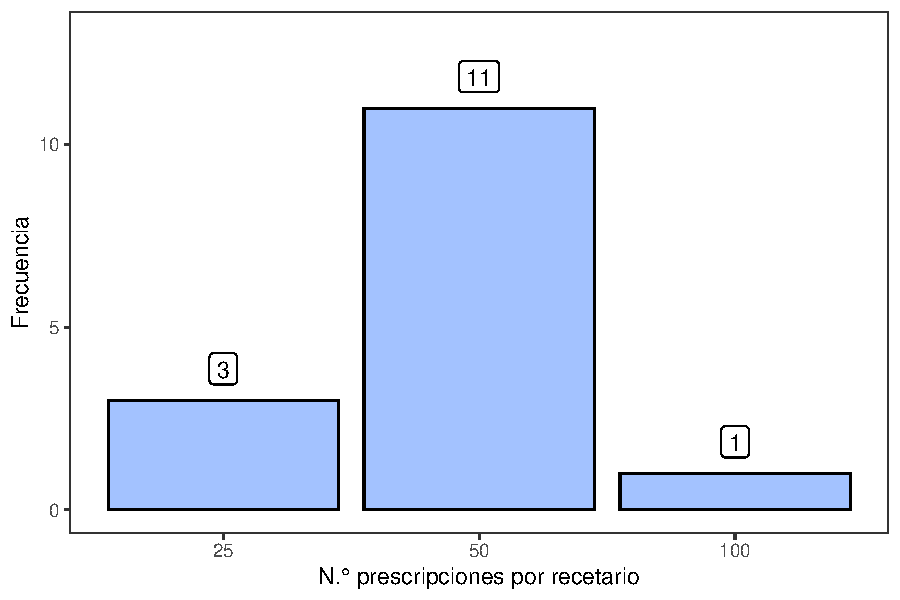
\includegraphics[width=0.85\linewidth]{InformeFinal_files/figure-latex/existenciaRecetarios4-1} 

}

\caption{N.° de prescripciones por recetario.}\label{fig:existenciaRecetarios4}
\end{figure}

\hypertarget{medidas-de-seguridad}{%
\subsection{Medidas de seguridad}\label{medidas-de-seguridad}}

Uno de los puntos de acompañamiento del proyecto Misión PRI 1901 era conocer tanto en las visitas presenciales como virtuales, los tipos de medidas de seguridad que se implementan en los recetarios. La Figura \ref{fig:MedidasSeguridadRec} contempló lo mencionado anteriormente, en la cual se observa que existe una gran variedad de medidas consideradas de seguridad en los recetarios, y que existen y existirán tantas como proponentes se tengan. Así mismo, se catalogaron las medidas de seguridad en baja y alta complejidad, teniendo como base lo difícil que pueden llegar a ser falsificados. Se reconoce que todos los departamentos implementaron la codificación en los recetarios oficiales tal y como se menciona en la Resolución 1478 de 2008\textsuperscript{\protect\hyperlink{ref-MSPS1478-2006}{1}} en el Artículo 89 y dicha codificación desarrollada para cada talonario está pensada para ser una identificación única de los mismos.
Tanto como la codificación como las marcas de agua, sellos y escudos se catalogaron como medidas de seguridad de baja complejidad, teniendo en cuenta que hay un riesgo latente de falsificación debido a que las marcas de agua corresponden a figuras particulares o al escudo de la gobernación y/o secretaria de salud, al igual que los sellos y escudos. Sumado a lo anterior, los recetarios están elaborados en papel común y corriente, lo que podría aumentar la probabilidad de ser falsificados.

\begin{figure}

{\centering 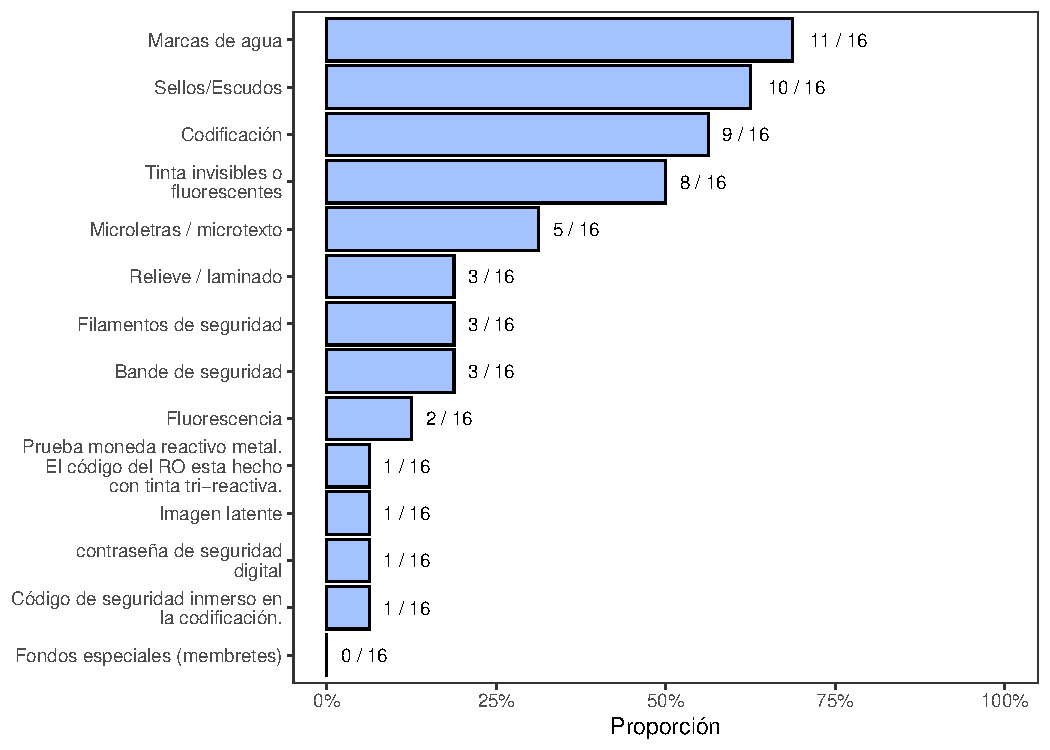
\includegraphics[width=0.9\linewidth]{InformeFinal_files/figure-latex/MedidasSeguridadRec-1} 

}

\caption{Medidas de seguridad en los recetarios.}\label{fig:MedidasSeguridadRec}
\end{figure}

Considerando lo anterior, los FRE han optado por implementar niveles de seguridad mayores y elevar la confianza en el manejo de los recetarios, entre estas medidas se observan las siguientes:

\begin{itemize}
\item
  Tintas invisibles o fluorescentes que brillan al estar frente a la luz UV.
\item
  Microletras/microtextos, los cuales están inmersos en cada folio del recetario donde se describe para quien va cada copia.
\item
  Relieves o laminados observados en la copia original de los recetarios.
\item
  Filamentos o bandas de seguridad tecnología similar a los billetes.
\item
  Pruebas reactivo metal, que consisten en raspar un espacio determinado del recetario con un metal o moneda desde la página original del mismo y automáticamente los folios continuos se marcarán.
\item
  Códigos QR que codifican información del año en el cual fue distribuido el talonario.
\end{itemize}

Menos del 40\% de los FRE han implementado medidas de alta seguridad en sus recetarios debido a la capacidad de manufactura de los proveedores departamentales. Dicha limitante se identificó en especial en las regiones alejadas del centro del país, donde en términos de los FRE, los proveedores departamentales no tienen la capacidad o la tecnología suficiente para elaborar un talonario con características de alta seguridad. Además, adquirir contratos con proveedores externos al departamento dificulta el seguimiento o alarga los procesos de compra, por lo que supone superar las barreras geográficas y/o sociales de algunos departamentos.

Al inicio del proyecto de inversión, se estimaba que los recetarios oficiales con más características de seguridad (independiente de su nivel de complejidad) aumentarían de forma proporcional su costo de adquisición y del mismo modo su precio de venta, sin embargo, se evidenció una tendencia totalmente diferente que se puede observar en la Figura \ref{fig:ComparativoCostosRec1} y Figura \ref{fig:DependParcial1}, entre más características de seguridad implementadas en un recetario, éste tiende a ser más económico en su costo de adquisición.

\begin{figure}

{\centering 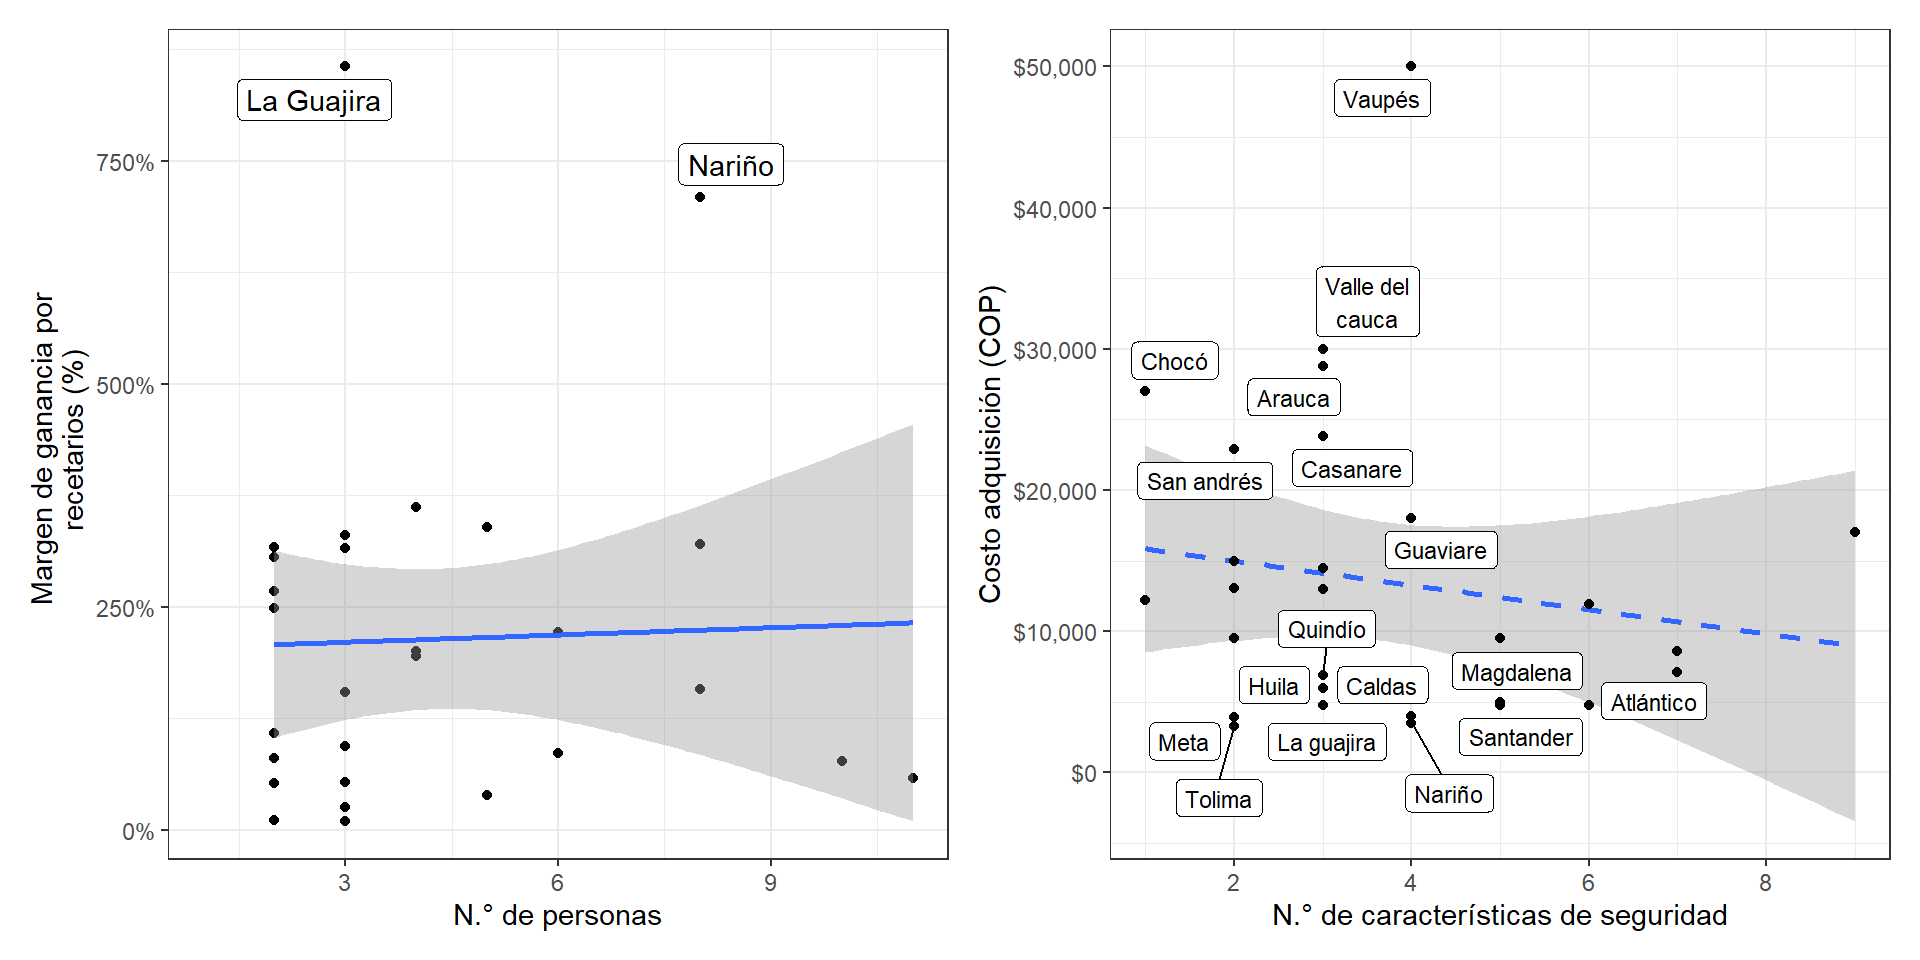
\includegraphics[width=1\linewidth]{InformeFinal_files/figure-latex/ComparativoCostosRec1-1} 

}

\caption{Comparativo de márgen de ganancia de recetarios.}\label{fig:ComparativoCostosRec1}
\end{figure}

Por otro lado, se observa el margen de ganancia obtenido mediante la venta de recetarios en los fondos rotatorios, este ítem ya se analizó anteriormente con la Figura \ref{fig:comparativoDepartamentos0}. Sin embargo, no se encuentra una relación entre este margen de ganancia con el número de personas que trabajan dentro del FRE.

Si bien las ganancias obtenidas por las ventas de recetarios son unas de las fuentes principales de ingresos en los entes territoriales, no hay claridad de cómo se manejan estos valores debido a que departamentos con los mismos márgenes de ganancia tienen condiciones distintas, tanto en personal como en infraestructura tecnológica y estructural.

\hypertarget{recetario-oficial-electruxf3nico}{%
\section{Recetario Oficial Electrónico}\label{recetario-oficial-electruxf3nico}}

El recetario oficial electrónico (ROE) es una herramienta que busca generar un mecanismo de prescripción estandarizado en el territorio nacional para los medicamentos de control especial (MCE) donde se reúna tanto las prescripciones de uso humano como veterinario. Se espera que constituya un mecanismo integrado a una plataforma como lo es MIPRES (ya implementada y con amplio acceso), permitiendo un mayor seguimiento y control sobre los regímenes actualmente cubiertos por el aplicativo, incluyendo los procesos de información sobre la dispensación de estos productos farmacéuticos y generando la información necesaria para tener un seguimiento y análisis de prescripciones y dispensaciones de MCE en el territorio nacional\textsuperscript{\protect\hyperlink{ref-CuervoBustamante2021}{13}}.

\hypertarget{opiniones-sobre-el-roe}{%
\subsection{Opiniones sobre el ROE}\label{opiniones-sobre-el-roe}}

\begin{figure}[t]

{\centering 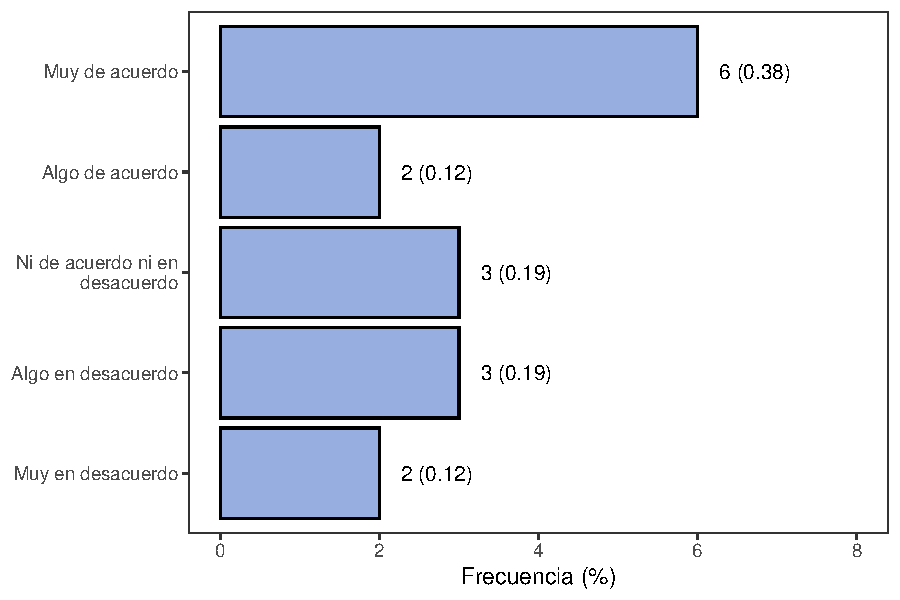
\includegraphics[width=0.85\linewidth]{InformeFinal_files/figure-latex/FREImplementacionROE-1} 

}

\caption{Opinión sobre la implementación del Recetario Oficial Electrónico (ROE).}\label{fig:FREImplementacionROE}
\end{figure}

Como se observa en la Figura \ref{fig:FREImplementacionROE}, el 58\% de los FRE del país tienen una opinión favorable acerca del ROE, ya que, según la información recopilada, los encargados de los diferentes FRE piensan que podría ser una herramienta que brinde mayor seguimiento, trazabilidad y seguridad a las prescripciones de MME, además del ahorro de papel y de espacio de almacenamiento en las bodegas que sería liberado. Como ejemplo de opinión positiva respecto a la implementación del FRE se tiene:

\begin{quote}
\emph{``\ldots{} puede ser un proceso interesante para llevar trazabilidad de los recetarios oficiales. El recetario oficial actual es insuficiente para hacer el respectivo seguimiento y control. Igualmente, el ROE podría mejorar la accesibilidad de medicamentos.''}
\end{quote}

Por otro lado, 29\% de los FRE del país tienen una percepción no favorable acerca de la implementación del ROE principalmente por razones económicas, ya que al dejar a un lado la venta de recetarios oficiales físicos se perdería ese rubro de ingresos al FRE. Adicionalmente, algunos referentes de los entes territoriales manifiestan preocupación por las posibles violaciones de acceso a personal no autorizado, además de los FRE limítrofes, ubicados en regiones con deficiente conexión, afirman que no tendrían la capacidad tecnológica para desarrollar la prescripción por ROE permanentemente a lo que comentan que como medida de contingencia, debería seguir existiendo el recetario oficial en físico, como medida de prevención cuando se pierda acceso a internet en sus territorios, lo que indica la necesidad de realizar campañas de capacitación y educación de uso del ROE antes y durante su implementación como medida prioritaria para el desarrollo de la herramienta digital.

Como ejemplo de opinión negativa se tiene:

\begin{quote}
\emph{``La razón principal es el factor financiero. El FRE necesita los ingresos generados por los recetarios oficiales propios, para su sostenimiento. Igualmente, es difícil continuar con las actividades de seguimiento y control para los recetarios oficiales. Así mismo, podría prestarse para un manejo inadecuado de los MME, contemplando fraude y desvíos en los recetarios oficiales electrónicos.''}
\end{quote}

\hypertarget{manejo-de-medicamentos}{%
\chapter{Manejo de Medicamentos}\label{manejo-de-medicamentos}}

\maxdeadcycles=1000

El artículo 6 de la Resolución 1478 de 2006\textsuperscript{\protect\hyperlink{ref-MSPS1478-2006}{1}} refiere las sustancias y los medicamentos fabricados con las mismas que pertenece al monopolio del Estado. Este listado de sustancias se ha modificado mediante la Resolución 262 de 2009\textsuperscript{\protect\hyperlink{ref-MSPS262-2009}{14}} y la Resolución 940 de 2007\textsuperscript{\protect\hyperlink{ref-MSPS940-2007}{15}}, en el sentido de modificar las hojas de coca por cocaína con fines terapéuticos, e incluir a la primidona en todas sus presentaciones de manera respectiva.

Es así, que el FNE cuenta con el Grupo Interno de Trabajo de Medicamentos del Estado que tiene como objetivo Garantizar la disponibilidad de los medicamentos del Estado de manera oportuna y eficiente en todo el territorio Nacional.

Actualmente, el FNE ofrece un portafolio de medicamentos monopolio del Estado (MME) como se muestra en la Tabla \ref{tab:portafolioMME}\textsuperscript{\protect\hyperlink{ref-ColombiaCompraEficiente2021}{16}}.

\begin{table}[!h]

\caption{\label{tab:portafolioMME}Portafolio de Medicamentos Monopolio del Estado.}
\centering
\begin{tabular}[t!]{lcc}
\toprule
Producto & Presentación & Observaciones\\
\midrule
Fenobarbital Sol Oral 0,4\% & Frasco & Disponible\\
Fenobarbital 10 mg & Caja 30 tabletas & Disponible\\
Fenobarbital 50 mg & Caja 30 tabletas & Disponible\\
Fenobarbital 100 mg & Caja 30 tabletas & Disponible\\
Fenobarbital 40 mg & Caja 10 ampollas & Disponible\\
\addlinespace
Fenobarbital 200 mg & Caja 10 ampollas & Disponible\\
Hidromorfona HCL 2 mg & Caja 10 ampollas & Disponible\\
Hidromorfona HCL 2.5 mg & Caja 20 tabletas & Disponible\\
Meperidina HCL 100 mg & Caja 10 ampollas & Disponible\\
Morfina HCL 10 mg & Caja 10 ampollas & Disponible\\
\addlinespace
Morfina Solución Oral & Frasco & Disponible\\
Morfina Solución Vial & Frasco & Sin unidades disponibles\\
Primidona 250 mg & Caja 50 tabletas & Sin unidades disponibles\\
Primidona 250 mg Tabletas & Caja x 30 Tabletas & Disponible\\
Metadona HCL 10 mg & Frasco 20 tabletas & Disponible\\
\addlinespace
Metadona HCL 10 mg & Caja 30 tabletas & Disponible\\
Metadona HCL 40 mg & Frasco 20 tabletas & Disponible\\
Metadona HCL 40 mg & Caja x 30 tab & Disponible\\
Metilfenidato HCL 10 mg & Caja 30 tabletas & Disponible\\
Metilfenidato LA 30 mg & Frasco 30 capsulas & Disponible\\
\addlinespace
Metilfenidato 18 mg & Frasco 30 tabletas & Disponible\\
Metilfenidato 36 mg & Frasco 30 tabletas & Disponible\\
Hidrato de Cloral 10\% Solución oral & Frasco & Disponible\\
Morfina HCL 10 mg ampolla x 5 mL & Caja 5 ampollas & Disponible\\
\bottomrule
\end{tabular}
\end{table}

Los medicamentos incluidos en el portafolio de medicamentos del Estado son importantes en el tratamiento de diversas enfermedades de alto impacto en la salud de la población colombiana. En el área de cuidados paliativos se tienen a los medicamentos con morfina, metadona, meperidina e hidromorfona como parte importante del tratamiento del dolor crónico. Algunas sociedades científicas relacionadas a esta área han encontrado barreras en la entrega efectiva de medicamentos opioides, así como una distribución inequitativa en el territorio nacional de los mismos\textsuperscript{\protect\hyperlink{ref-LeonDelgado2018}{17}}.

Pese a todo esto, Colombia tiene una puntuación de 4 de 5 en la escala de colaboración entre prescriptores y reguladores de analgésicos opioides (para Latinoamérica), lo que resulta de la existencia de mecanismos de colaboración pese a que todavía se pueden realizar mejoras en los mismos\textsuperscript{\protect\hyperlink{ref-Pastrana2020}{18}}.

Así mismo el fenobarbital se considera una alternativa terapéutica útil en el tratamiento de epilepsia refractaria\textsuperscript{\protect\hyperlink{ref-WatsonLewis2014}{19}}, o estatus convulsivo\textsuperscript{\protect\hyperlink{ref-VergaraAguilar2019}{20}}. La primidona cuenta con un espacio limitado en la terapia moderna de la epilepsia\textsuperscript{\protect\hyperlink{ref-Johannessen2020}{21}}, y algunos pacientes todavía requieren un suministro ininterrupido de la misma. Por otra parte, el metilfenidato es un componente importante en el tratamiento farmacológico de los trastornos por deficit de atención, los cuales tienen una prevalencia en la población colombiana\textsuperscript{\protect\hyperlink{ref-Pineda2001}{22},\protect\hyperlink{ref-Llanos-Lizcanoa2019}{23}}.

Sí bien el establecimiento de un monopolio del Estado con estos medicamentos ha permitido el suministro de los mismos debido a que pueden ser poco atractivos por ser medicamentos menos rentables, la restricción de un mercado de libre competencia puede resultar en el surgimiento frecuente de eventos de desabastecimiento\textsuperscript{\protect\hyperlink{ref-LopezLopez2021}{24},\protect\hyperlink{ref-INVIMA2018-Desabast}{25}}.

Los desabastecimientos son situaciones en la cual se presenta una insuficiente oferta para satisfacer la demanda de un producto farmacéutico que ya ha sido aprobado por el INVIMA y comercializado en el país\textsuperscript{\protect\hyperlink{ref-INVIMA2018-Desabast}{25}}.

Por lo general, los desabastecimientos se ven precedidos por disrupciones en la cadena de suministro\textsuperscript{\protect\hyperlink{ref-FDA2014}{26}}. Las \emph{disrupciones en la cadena de suministro} se definen como eventos aleatorios que causan que un fabricante u otro elemento de la cadena de suministro pare de funcionar de forma completa o parcial por una cantidad de tiempo (aleatoria)\textsuperscript{\protect\hyperlink{ref-Barbosa-Povoa2019}{27}}. Las instituciones deben establecer programas de gestión del riesgo también aplicadas a la cadena de suministro, en estas se busca mitigar riesgo de suministro/demanda y disrupción. Por otra parte, la \textbf{resiliencia} se puede definir como la habilidad de sobrevivir, adaptarse y crecer tras un cambio turbulento. La implementación de programas de gestión de resiliencia en la cadena de suministro se centra en la habilidad de aprender y crecer tras las disrupciones de la cadena de suministro\textsuperscript{\protect\hyperlink{ref-Barbosa-Povoa2019}{27}}.

La resiliencia de una cadena de suministro, como lo es la distribución de MME, se puede mejorar mediante la construcción de capacidades teniendo en cuenta vulnerabilidades\textsuperscript{\protect\hyperlink{ref-Pettit2013}{28}}. Una de estas capacidades es la visibilidad referida al conocimiento del estado operativo de la cadena y su medio circundante\textsuperscript{\protect\hyperlink{ref-Pettit2013}{28}}. El \emph{intercambio de información} es una de las áreas en las que se pueden realizar mejoras para potenciar la coordinación en una cadena de suministro\textsuperscript{\protect\hyperlink{ref-Silver2017}{29}}.

La falta de transparencia y visibilidad en una cadena de suministro puede causar el efecto látigo (en inglés, \emph{Bullwhip effect}) que consiste en un aumento de la variabilidad en la demanda de un sitio corriente abajo de la cadena a un sitio corriente arriba de la misma\textsuperscript{\protect\hyperlink{ref-Cachon2007}{30}}. Este efecto implica que se pueden generar condiciones de alta incertidumbre que llevan a una mala planeación y esto a desabastecimientos o pérdidas por vencimiento de MME tanto para el FNE como para los FRE.

Es por esto, que tanto el FNE como los FRE - en conjunto - deberían implementar, por ejemplo, un sistema de Planeamiento Participativo, Pronóstico y Reabastecimiento (CPFR, \emph{Collaborative Planning Forecasting and Replenishment}) de manera que exista una colaboración más robusta y visible de la cadena de suministro de medicamentos Monopolio del Estado\textsuperscript{\protect\hyperlink{ref-Hollmann2015}{31}}.

Debido a la necesidad de fortalecer la cadena de suministro de MME, en este capítulo se muestran los resultados relacionados a medicamentos obtenidos en la encuestas aplicadas, con el fin de evidenciar algunos aspectos operativos relacionados al manejo de medicamentos en los FRE.

\hypertarget{inventarios}{%
\section{Inventarios}\label{inventarios}}

\maxdeadcycles=1000

El manejo de inventarios es de gran relevancia para las organizaciones que tienen bienes tangibles dispuestos a la venta como lo son los FRE. Los inventarios son necesarios debido a la presencia de incertidumbres relacionadas a la demanda de los productos, tiempos de demora en el reabastecimiento, suministro por parte de los proveedores (p.ej. FNE), precio de los medicamentos, cambios en el personal, tiempos de tránsito, entre otros factores\textsuperscript{\protect\hyperlink{ref-Nahmias2007}{32}}.

En la selección del tamaño de inventario a mantener se contraponen varios tipos de costos\textsuperscript{\protect\hyperlink{ref-Krajewski2016}{33}}:

\begin{itemize}
\item
  Costo de mantenimiento de inventario (lleva a reducir el inventario): compuesto por el costo de capital (relacionado a la pérdida de oportunidad de invertir dinero en inventario en vez de una alternativa con más rentabilidad), costos por almacenamiento (p.ej. arriendo, servicios públicos, o seguros), costos de empleados (p.ej. mantenimiento, administración, alistamiento o auditoría), costos por servicios (seguros, seguridad privada, software de administración de inventario), costos de riesgo de inventario (depreciación, vencimientos, contracción de la demanda).
\item
  Costo de pedido (lleva a aumentar el inventario): costos por ordenes de compra (relacionados a la cotización, preparación de órden de compra, tiempo de recepción técnica, pagos), y costos por personal relacionado a la compra.
\item
  Costos por desabastecimiento (lleva a aumentar el inventario): relacionado al \textbf{nivel de servicio}, entendido como la probabilidad deseada de no tener un desabastecimiento durante el reabastecimiento de los productos (de manera que se pueda cumplir con las demandas de los usuarios en todo momento)\textsuperscript{\protect\hyperlink{ref-Krajewski2016}{33}}.
\end{itemize}

\hypertarget{control-de-inventarios}{%
\subsection{Control de inventarios}\label{control-de-inventarios}}

La implementación de un software de manejo de inventarios o en el mejor de los casos de un ERP (\emph{Enterprise Resource Planning}) mejora la capacidad de manejar los inventarios, disminuye costos relacionados a inventario y brinda oportunidad para la coordinación\textsuperscript{\protect\hyperlink{ref-Silver2017}{29}}. Se indago a los FRE sobre las herramientas que tienen a disposición para el manejo de inventarios de MME. La mayoría de los FRE realizan el seguimiento de inventarios mediante un paquete ofimático con una proporción de 45.2\% (ver Figura \ref{fig:HerramientasManejoInventarios}), siendo la herramienta principal Excel, con uso especial de hojas estandarizadas, como en el caso de los FRE Boyacá, Cauca, Sucre, entre otros.

\begin{figure}[t]

{\centering 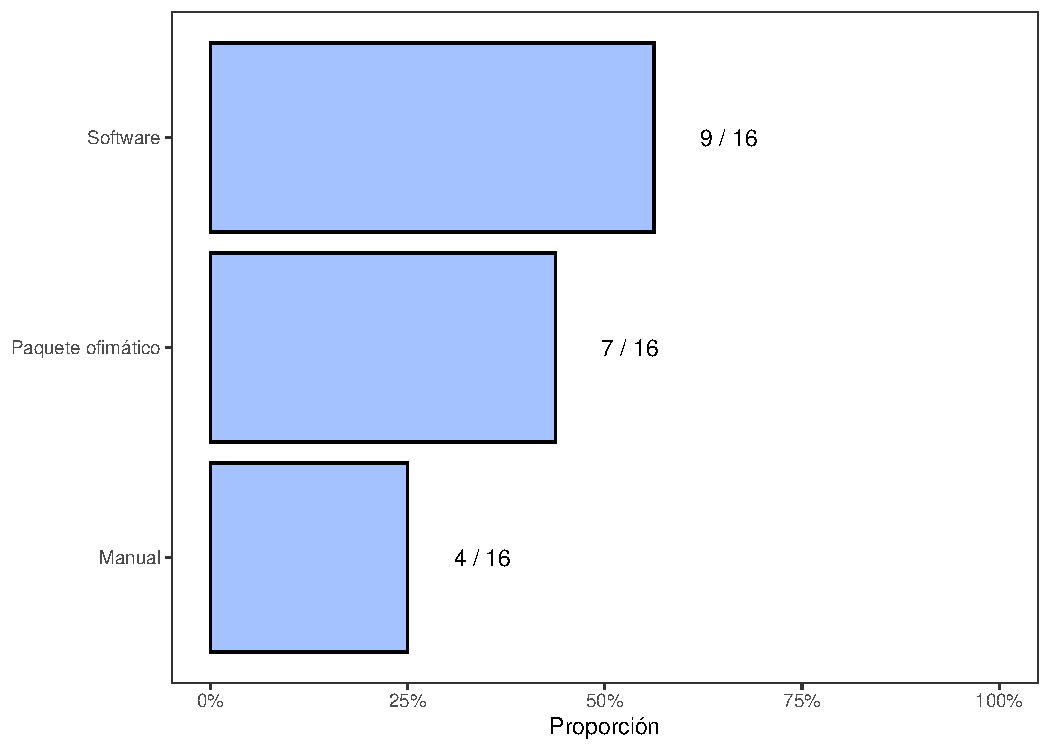
\includegraphics[width=0.95\linewidth]{InformeFinal_files/figure-latex/HerramientasManejoInventarios-1} 

}

\caption{Herramientas en el manejo de inventarios.}\label{fig:HerramientasManejoInventarios}
\end{figure}

Algunos FRE se apoyan en otras herramientas además del paquete ofimático para llevar a cabo la tarea del control de inventarios. En la segunda posición de la Figura \ref{fig:HerramientasManejoInventarios} se observa el uso de software en una proporción del 38.7\%. La elección del software se hace según los criterios de cada entidad territorial en la mayoría de los casos se utiliza un software interno de la gobernación del territorio para el desarrollo de estas actividades como es el caso de los FRE Atlántico, Cesar, Santander, entre otros.

El alcance del software es distinto, por ejemplo, el caso del FRE Risaralda que hace uso del software SIMEC para soportar tanto el manejo de inventarios, como los procesos relacionados con el sistema de IVC en todo lo relacionado con MME. Este software funciona además como medio de comunicación entre el FRE y todos sus inscritos, mostrándose como una plataforma muy completa y eficiente, sin embargo, existe poca disponibilidad de equipos de cómputo en el FRE que impide que más personal pueda acceder al software y a sus herramientas por lo cual puede ser un recurso subutilizado.

Se evidencia que algunos FRE poseen herramientas completas para el manejo de sus procesos, mientras que otros realizan el manejo de inventarios apoyándose en el uso de herramientas manuales (32.3\%), como se indica en la Figura \ref{fig:HerramientasManejoInventarios} En muchos FRE el control de inventarios de forma manual se realiza con apoyo de herramientas ofimáticas como Excel.

Sólo en tres casos se encontró que el control de inventarios dependía exclusivamente de herramientas manuales como la revisión de libros contables. Pese a que no es el ideal algunos territorios, especialmente los menos centralizados (p.ej. Amazonas y La Guajira), se ven en la necesidad de llevar sus procesos de esta forma debido a la no disponibilidad de equipos de cómputo o que sí bien los hay, esto se encuentran obsoletos y no soportan el uso de tecnologías más recientes y apropiadas.

Finalmente, el manejo de inventarios por parte de los FRE deja en evidencia las brechas tecnológicas importantes entre los territorios. Los FRE menos centralizados presentan menor acceso a tecnologías actualizadas y en estos fue común encontrar la necesidad de acceso a más equipos de cómputo que le permita al personal desarrollar las actividades para el funcionamiento del FRE.

Por todo esto se recomienda el uso de herramientas informáticas para la trazabilidad del inventario.

\hypertarget{comportamiento-de-compra-de-fre}{%
\subsection{Comportamiento de compra de FRE}\label{comportamiento-de-compra-de-fre}}

De forma ideal se debería tener en cuenta el balance entre los costos de mantenimiento de inventario y los costos de realizar pedidos para encontrar una cantidad económica de pedido (\(\mathrm{EOQ}\), \emph{Economic Order Quantity}). Para realizar una programación de compras anuales se debería tener en cuenta la demanda anual del producto y dividirla entre \(\mathrm{EOQ}\), de esta manera se puede encontrar el número de pedidos óptimos\textsuperscript{\protect\hyperlink{ref-Silver2017}{29}}.

El número de pedidos (compras) de MME al FNE en el año también depende de varios factores como: (a) cantidad requerida de estos bienes por cada departamento (demanda), (b) presupuesto asignado por las gobernaciones a los FRE y (c) capacidad de satisfacer la demanda de los medicamentos por parte del FNE (ver Figura \ref{fig:FrecComprasFNR}).

Los FRE con demandas pequeñas de medicamentos, como es el caso de Choco, Guainía y Amazonas, la compra se hace una vez al año, a menos que enfrenten casos de desabastecimiento por causas fortuitas como lo fue la situación de Emergencia Sanitaria por la pandemia de coronavirus. Los departamentos con mayor población y necesidad de medicamentos se ven en la obligación de realizar varias compras en el año como es el caso del departamento de Antioquia cuya intención es realizar compras proyectando un abastecimiento de tres meses, sin embargo, manifiesta que el proceso se ve entorpecido por el bajo nivel de servicio relacionado a la disponibilidad de medicamentos en el FNE que le permitan satisfacer su demanda. Se presenta un caso similar para el FRE Santander, donde también afirman que la disponibilidad de medicamentos por parte del FNE es muy poca para cubrir la demanda de su departamento, por lo que obligatoriamente deben autorizar a las IPS y demás a hacer compras directas al FNE.

Por otra parte, hay departamentos donde la frecuencia de las compras y las cantidades de esta depende del presupuesto asignado por la gobernación, como es el caso de Guainía y Putumayo, este último indica que la demanda de MME en su territorio es más alta de la que se puede cubrir por limitaciones presupuestales.

Por su parte, otros territorios no pueden realizar las compras con las frecuencias que requieren por problemas administrativos o económicos de alguna índole que corresponden a la gobernación, como han manifestado los FRE de San Andrés, Atlántico y Huila.

\begin{figure}[t]

{\centering 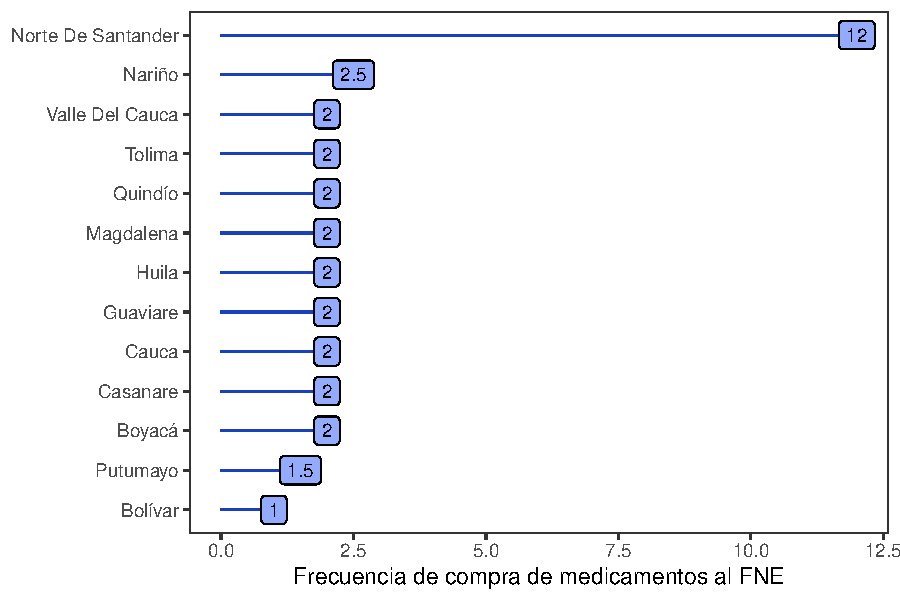
\includegraphics[width=0.9\linewidth]{InformeFinal_files/figure-latex/FrecComprasFNR-1} 

}

\caption{Frecuencia de compras de medicamentos por año al FNE.}\label{fig:FrecComprasFNR}
\end{figure}

\hypertarget{niveles-de-seguridad}{%
\subsection{Niveles de seguridad}\label{niveles-de-seguridad}}

Según la Resolución 1403 de 2007\textsuperscript{\protect\hyperlink{ref-MinisteriodeSaludyProteccionSocial2007}{34}}, donde se menciona el control durante el proceso de almacenamiento se encuentra que:

\begin{quote}
\emph{``El \ldots{} establecimiento farmacéutico contará con criterios, procedimientos y recursos que permitan calcular las existencias necesarias para un período determinado, fijando los niveles mínimo y máximo de existencias, punto de reposición o punto de pedido y presupuesto necesario para cumplir con la prestación oportuna del servicio. Se podrán utilizar aquellos indicadores que vayan surgiendo y que permitan realizar un exacto control de existencias''.}\textsuperscript{\protect\hyperlink{ref-MinisteriodeSaludyProteccionSocial2007}{34}}
\end{quote}

Con esto cabe aclarar que el control de existencias depende del criterio de cada organización, según como estas manejen sus productos. Se evalúo el uso de niveles de seguridad del inventario en los FRE. Un \textbf{inventario de seguridad} es una cantidad (nivel) almacenada adicional de producto que protege frente a incertidumbres en la demanda (\(D\)), tiempo de espera (\(L\)) o cambios en el suministro\textsuperscript{\protect\hyperlink{ref-Krajewski2016}{33}}. Los inventarios de seguridad se construyen basados en medidas de nivel de servicio que se encuentran relacionadas ya sea con costos de desabastecimiento o la probabilidad de desabastecerse\textsuperscript{\protect\hyperlink{ref-Silver2017}{29}}.

\begin{figure}

{\centering 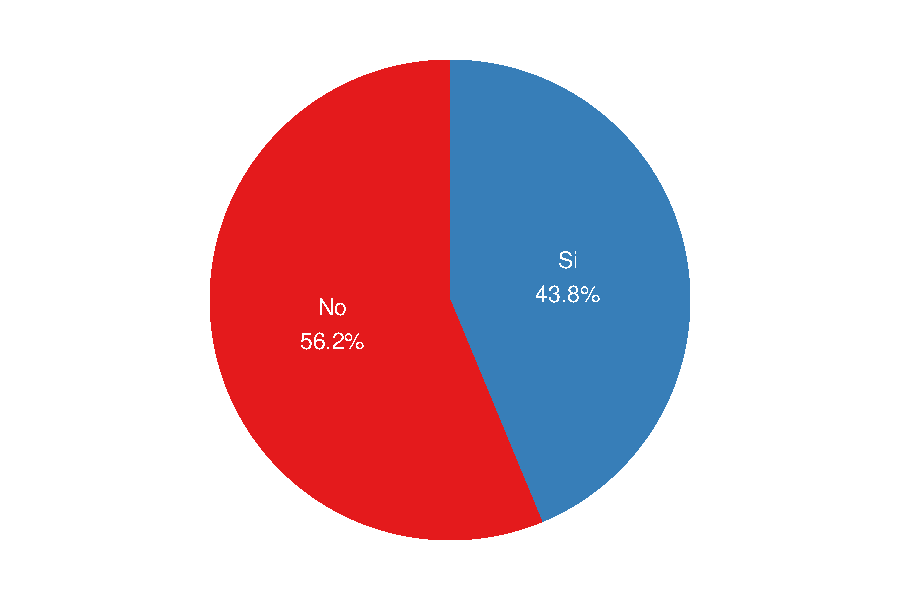
\includegraphics[width=0.78\linewidth]{InformeFinal_files/figure-latex/UsoNivelesSeguridad-1} 

}

\caption{Uso de niveles de seguridad del inventarios.}\label{fig:UsoNivelesSeguridad}
\end{figure}

Según los resultados obtenidos el 51.6\% de los FREs si manejan niveles de seguridad en los inventarios, es decir que de los 31 FREs existentes solo 16 manejan esta práctica y los 15 restantes no la usan; entre las razones para el no uso de esta estrategia se encuentra que la cantidad de medicamentos que rotan en algunos territorios no es muy alto, por ende, con la experiencia adquirida se sabe en qué momento se debe empezar a realizar el proceso de pedido de medicamentos (como p.ej. Guainía o Guaviare).

En otros casos se ve que el personal del FRE considera que su contacto directo con diario con los medicamentos, les permite verificar el comportamiento y determinar el momento indicado para tomar alguna acción. Se concluye entonces que 16 FREs usan estrategias de manejo óptimos de inventario y los 15 restantes lo hacen de una manera tradicional y dada por la experiencia adquirida con los años que llevan manejando el FRE en su región.

\hypertarget{adquisiciuxf3n-de-mme}{%
\section{Adquisición de MME}\label{adquisiciuxf3n-de-mme}}

\hypertarget{tiempos-de-demora-en-el-proceso-de-adquisiciuxf3n}{%
\subsection{Tiempos de demora en el proceso de adquisición}\label{tiempos-de-demora-en-el-proceso-de-adquisiciuxf3n}}

El tiempo de demora para reabastecimiento (\(L\), \emph{lead time}) es el tiempo que pasa desde el momento en el que se decide generar un pedido hasta que está físicamente listo en el almacén para satisfacer la demanda de los clientes\textsuperscript{\protect\hyperlink{ref-Silver2017}{29}}. Para un manejo adecuado del inventario, se debe tener en cuenta este tiempo para realizar los pedidos con anticipación de manera que no se produzcan desabastecimientos de forma frecuente.

Los tiempos de demora suelen tener varios componentes, en el diseño de la encuesta se tuvo en cuenta un proceso de adquisición de MME mediante etapas, de forma general se consideraron cinco etapas del proceso:

\begin{enumerate}
\def\labelenumi{\arabic{enumi}.}
\item
  Estimación de necesidades
\item
  Precontractual
\item
  Contractual
\item
  Solicitud en la plataforma tecnológica
\item
  Despacho (tiempo de tránsito)
\end{enumerate}

En este caso la plataforma tecnológica es la tienda virtual del Estado Colombia Compra Eficiente. El proceso puede cambiar de acuerdo con las particularidades de cada territorio, y el tiempo de demora para llevar a cabo estos procesos puede ser fijo o aleatorio.

En la Figura \ref{fig:EtapasProcesoAdquisicion} se muestran los departamentos en órden de acuerdo al tiempo total para la adquisición de MME. Se tiene que los departamentos de Putumayo (296 días), San Andrés (250 días), Caldas (238 días), Córdoba (181 días) y Boyacá (174 días) son los que más tiempo toman en los procesos de adquisición. Se tiene un promedio entre todos los departamentos de 90.9 días para el cumplimiento del proceso de adquisición.

\begin{figure}[t]

{\centering 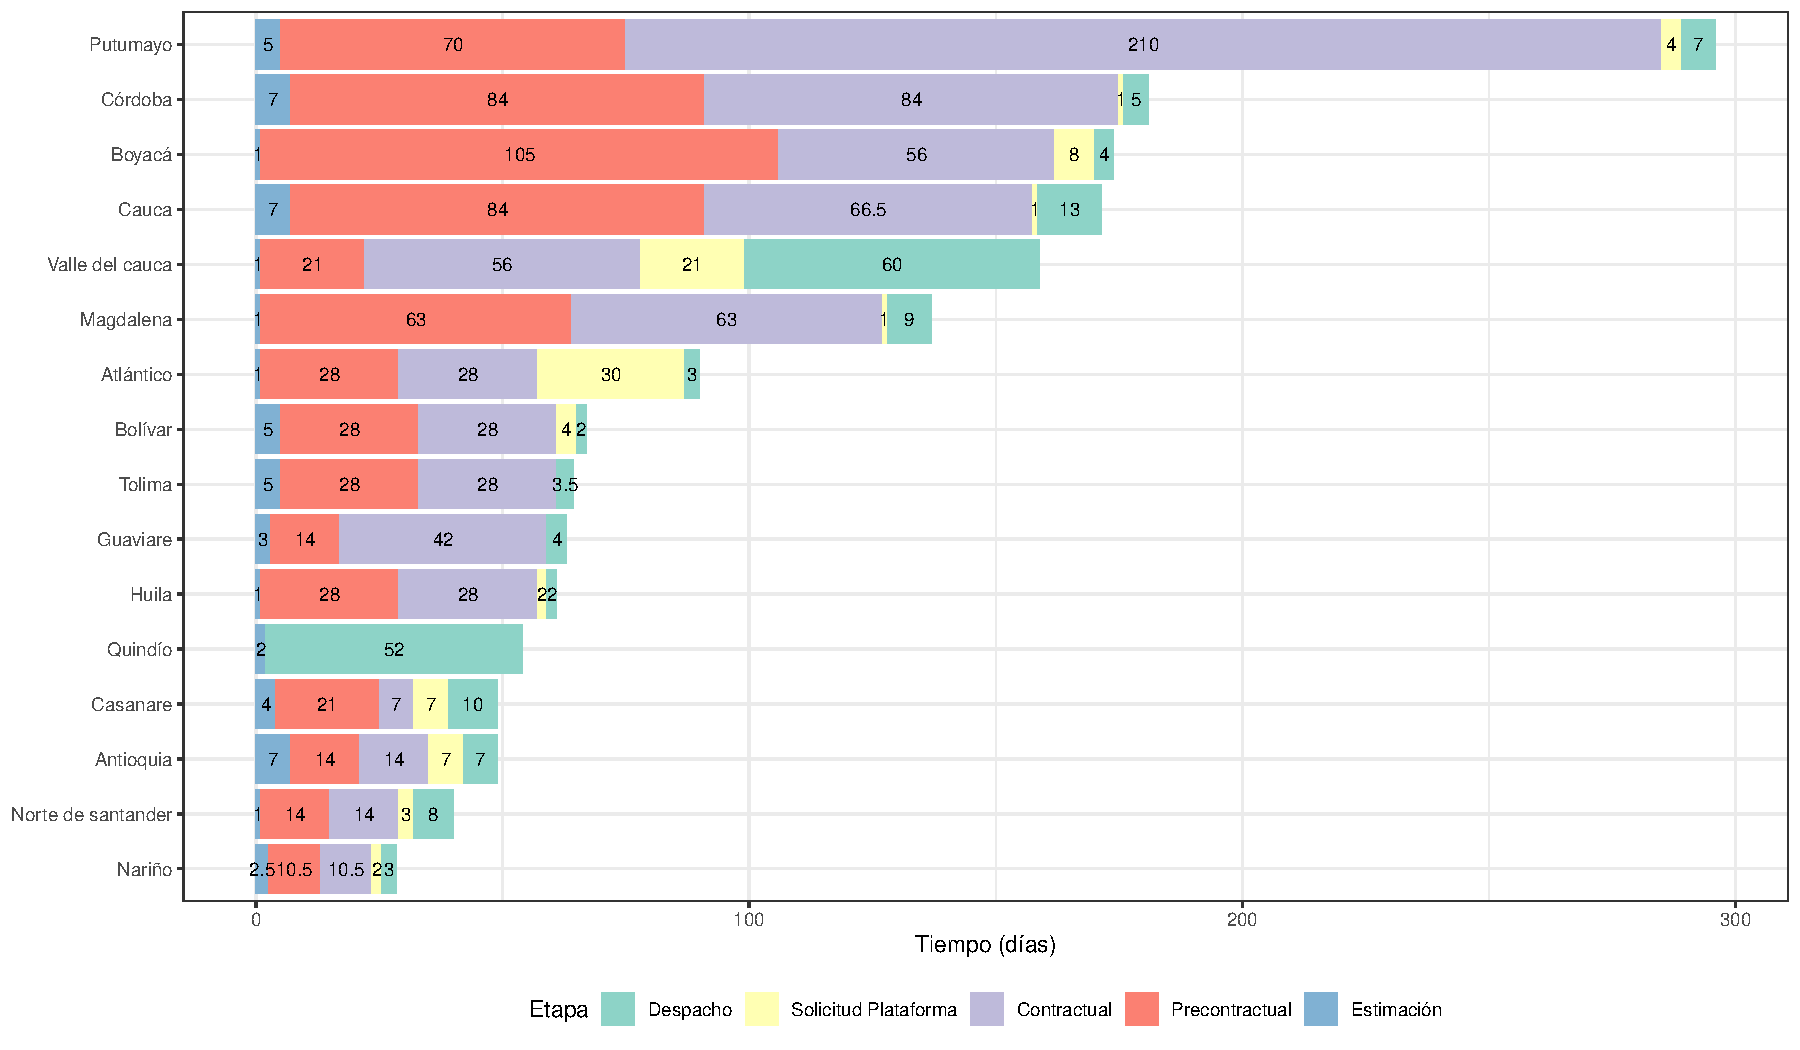
\includegraphics[width=1\linewidth]{InformeFinal_files/figure-latex/EtapasProcesoAdquisicion-1} 

}

\caption{Demoras en el proceso de adquisición por departamento.}\label{fig:EtapasProcesoAdquisicion}
\end{figure}

La diferencia en los tiempos para llevar a cabo los procesos de adquisición de MME (mostrados en la Figura \ref{fig:EtapasProcesoAdquisicion}) se puede explicar teniendo en cuenta factores como: (i) cantidad de medicamentos requeridos en cada departamento, (ii) herramientas usadas para el cálculo de la estimación de la necesidad, (iii) eficiencia u organización de los procesos contractuales de cada entidad y (iv) distancia física entre el FNE y la oficina del FRE. Este último factor puede afectar el tiempo de despacho de los MME de forma especial en las zonas más alejadas de la capital del país.

El proceso de estimación de compra de MME es uno de los más cortos (en promedio 3.31 días) y por lo general se hace teniendo en cuenta el consumo histórico en el territorio. El consumo histórico de medicamentos no es el único factor para tener en cuenta, es así como en el departamento de Casanare, el FRE además de revisar sus consumos históricos, consulta a sus inscritos la proyección de consumo de cada inscrito, adicionalmente agrega un 20\% a su proyección final para tener un inventario de seguridad que le permita evitar el desabastecimiento.

Por otra parte hay territorios como Guaviare en el que la estimación de compra sólo se hace teniendo en cuenta el consumo histórico y cuidando de no sobrepasar el presupuesto que la gobernación ha asignado para esta tarea. El FRE de Guaviare en comparación con otros territorios es pequeño, evidenciando que las necesidades y capacidades de los FRE son diferentes de acuerdo con el territorio.

Existen casos a exaltar como el FRE de Sucre que, a pesar de tener un tamaño relativamente pequeño a otros en la región, tiene un proceso de estimación de necesidades de MME está altamente estandarizado a través de una herramienta que facilita la toma de decisiones de compra de MME. El FRE afirma que el uso de este manual reduce el tiempo de estimación de compra a una semana, y esto indica que es un proceso eficiente en este departamento.

Como se identifica en la Figura \ref{fig:EtapasProcesoAdquisicionDetalle}, la gran mayoría de territorios manifiesta que las actividades que más tiempos requieren son las etapas precontractuales (en promedio 36.4 días) y contractuales (en promedio 46 días), esto debido a los requisitos que establece la contratación pública\textsuperscript{\protect\hyperlink{ref-CongresodelaRepublicadeColombia1993}{35},\protect\hyperlink{ref-CongresodelaRepublicadeColombia2007}{36}}. Para que una institución estatal pueda realizar una compra debe tener en cuenta la modalidad de contratación y los documentos exigidos en la misma, p.ej. los estudios previos en los que la entidad debe tener claridad sobre las especificaciones técnicas mínimas del servicio o bien a adquirir\textsuperscript{\protect\hyperlink{ref-CongresodelaRepublicadeColombia1993}{35}}. Por último, en la Figura \ref{fig:EtapasProcesoAdquisicionDetalle} se muestra la mediana y el rango intercuartílico de los tiempos de cada etapa del proceso.

\begin{figure}[t]

{\centering 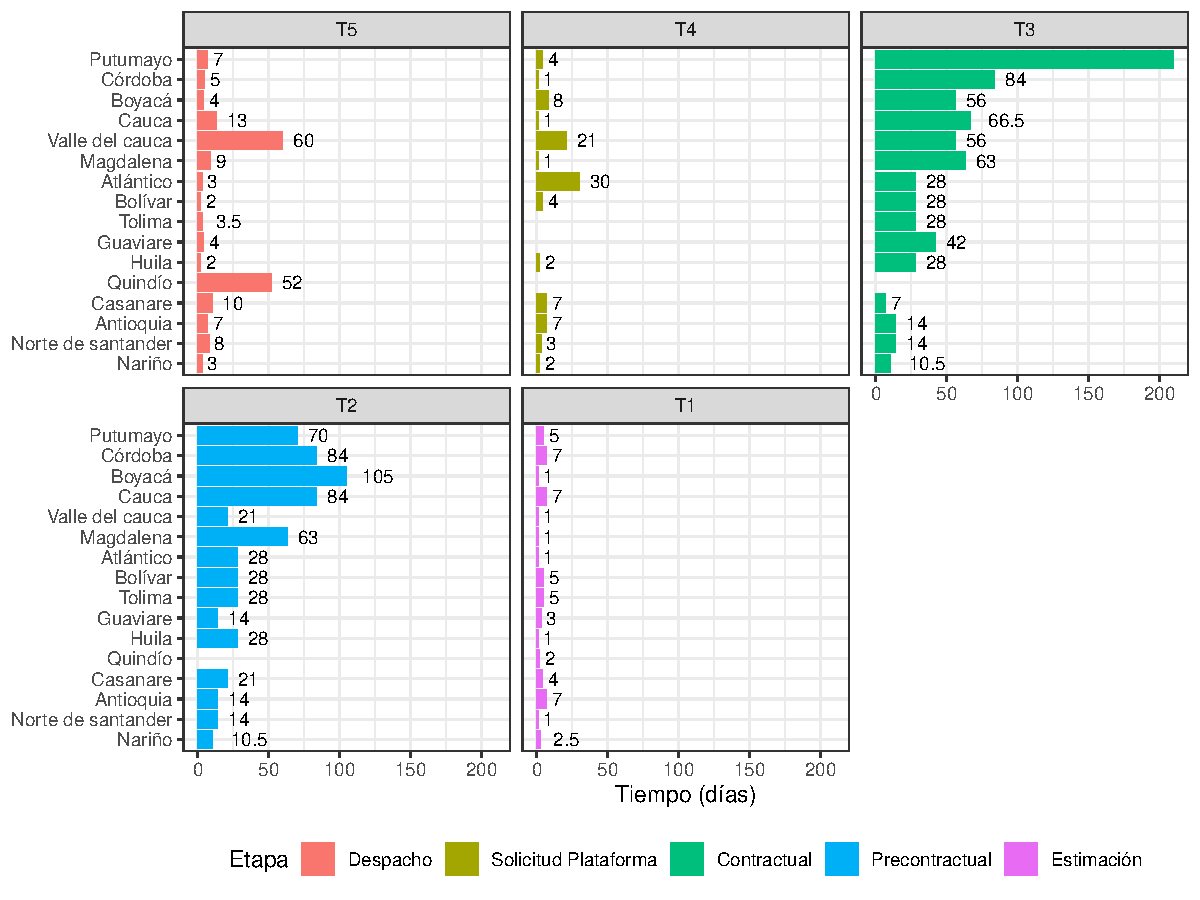
\includegraphics[width=0.95\linewidth]{InformeFinal_files/figure-latex/EtapasProcesoAdquisicionDetalle-1} 

}

\caption{Histogramas de tiempos en el proceso de adquisición por departamento. Línea negra segmentada mediana, líneas grises segmentadas primer y tercer cuartil.}\label{fig:EtapasProcesoAdquisicionDetalle}
\end{figure}

Por lo general, la documentación pertinente de la fase precontractual es revisada y corregida en varias ocasiones por diferentes áreas en una misma entidad, lo que conlleva a largos tiempos de espera en la fase precontractual. Estas demoras se dan especialmente cuando el área encargada de aprobar la documentación o de llevar a cabo el proceso contractual no pertenece a la secretaría de salud, como es el caso de Atlántico, pues los funcionarios de otras áreas de las gobernaciones no están inmersos en el contexto de las necesidades de salud pública y específicamente en la importancia que tiene el abastecimiento de MME para la población, por lo que muchas veces el proceso de adquisición de medicamentos queda a merced de la voluntad de otras áreas, propiciando incluso el desabastecimiento en los departamentos.

La etapa de solicitud en la plataforma tecnológica toma en promedio 6 días (mediana de 4 días). Los departamentos que reportan las mayores demoras en esta etapa son Atlántico (30 días) y Valle del Cauca (21 días), estos departamentos describieron problemas durante el proceso de compra mediante la plataforma. El resto de departamentos presentaban tiempos menores a 7 días para esta etapa.

La etapa de despacho tomó en promedio 10.4 días (mediana de 7 días). Los departamentos de Valle del Cauca (60 días), Quindío (52 días), y San Andrés (30 días) presentaron la mayor demora en esta etapa, estos tiempos reportados no parecen tener una relación cercana con la distancia física entre la oficina del FRE y el centro de despacho desde el FNE.

Los procesos relacionados a medicamentos esenciales como los son muchos MME no deben tener barreras que aumenten el riesgo de desabastecimientos\textsuperscript{\protect\hyperlink{ref-OMS2021}{37}}, estas barreras pueden estar relacionadas con los tiempos de demora. De acuerdo con lo evaluado se tiene que las etapas precontractuales y contractuales son las que más toman tiempo.

Los FRE deben propender por sensibilizar más a sus gobernaciones para que los procesos se realicen en tiempos más prudentes. Es deber de todos los actores relacionados a los procesos de medicamentos garantizar el acceso a los mismos por parte de la población, acorde a las políticas implementadas por el gobierno nacional\textsuperscript{\protect\hyperlink{ref-PDSPMinSalud2019}{38}}.

\hypertarget{plataforma-de-compra-estatal}{%
\subsection{Plataforma de compra estatal}\label{plataforma-de-compra-estatal}}

La plataforma Colombia Compra es el ente rector en materia de contratación pública y desde 2013 se puso en marcha la tienda virtual del Estado colombiano como herramienta en línea del sistema de compra pública. Esta plataforma permite hacer compras a través de acuerdos marco, instrumentos de agregación de demanda y catálogo de bienes de las grandes superficies. En concordancia con lo anterior, Colombia Compra Eficiente dispuso un documento en su plataforma denominado \emph{``Estudios y Documentos Previos de la contratación con el Fondo Nacional de Estupefacientes para la adquisición de Medicamentos de Control Especial de Monopolio del Estado''} donde afirma que se promueve un Instrumento de Agregación de Demanda de Precios para la adquisición de MME mediante contratación directa con el FNE, con el objetivo de aumentar la eficiencia en los procesos de cada FRE y aprovechar las economías a escala. Pese a su implementación y sus objetivos algunos FRE no perciben su uso como una ventaja.

De esta manera los FRE adquieren los MME a través de esta herramienta, por tal motivo se indagó sobre el uso de la plataforma y la opinión que tenían los FRE sobre la misma. Se encuentra que en términos generales (ver la Figura \ref{fig:EtapasProcesoAdquisicionDetalle}), que los FRE consideran que el tiempo invertido en el uso y trámite que se realiza a través de la plataforma, no es tan dispendioso como las etapas precontractuales y contractuales del proceso.

La mayoría de los departamentos hace uso de esta plataforma, encontrándose diferentes percepciones sobre ella. Por ejemplo, el FRE del Cauca indica alta satisfacción con el uso de la plataforma al considerar que es muy organizada, por otra parte el FRE del Valle del Cauca que indica inconformidad en el uso porque consideran que el mismo implica un extenso proceso precontractual y esto puede ser ineficiente y poco intuitivo. El FRE Meta afirma que en la plataforma existen factores que tardan en actualizarse como por ejemplo firmas de la secretaría de salud o incongruencias en el despacho de medicamentos comprados, y el FRE de Santander menciona que los precios en la plataforma suelen encontrarse desactualizados respecto a los del FNE.

Si bien el uso del Instrumento de Agregación de Demanda de precios dispuesto por Colombia Compra Eficiente para la adquisición de MME por parte de los FRE es de obligatoriedad, según la Circular Externa 005 de 2019 emitida por el FNE\textsuperscript{\protect\hyperlink{ref-FNE005-2019}{39}}, no todos llevan a cabo este proceso. Un caso podría ser el FRE Guainía que no ha utilizado la plataforma por falta de conocimiento sobre la misma y tiempo para capacitar a su personal respecto a ello, o el FRE Meta que expresa varias inconformidades sobre el uso de esta.

De otra parte, es necesario mencionar que, si bien casi todos los departamentos hacen uso de la plataforma, este proceso no siempre está a cargo del FRE, como en el caso del departamento del Atlántico, donde el proceso se lleva a través de Secretaría General y por ello su percepción sobre la misma es \emph{``ni conforme ni inconforme''}. Es así como en la Figura \ref{fig:ColombiaCompra} se identifica como la segunda respuesta más frecuente \emph{``Ni conforme ni inconforme''} con el uso de esta plataforma. De otra parte, el FRE Putumayo comenta que el uso de la plataforma depende en gran medida de otras áreas de la gobernación, evidenciando varias dificultades en su uso y aumentando el tiempo en los procesos de contratación.

\begin{figure}[t]

{\centering 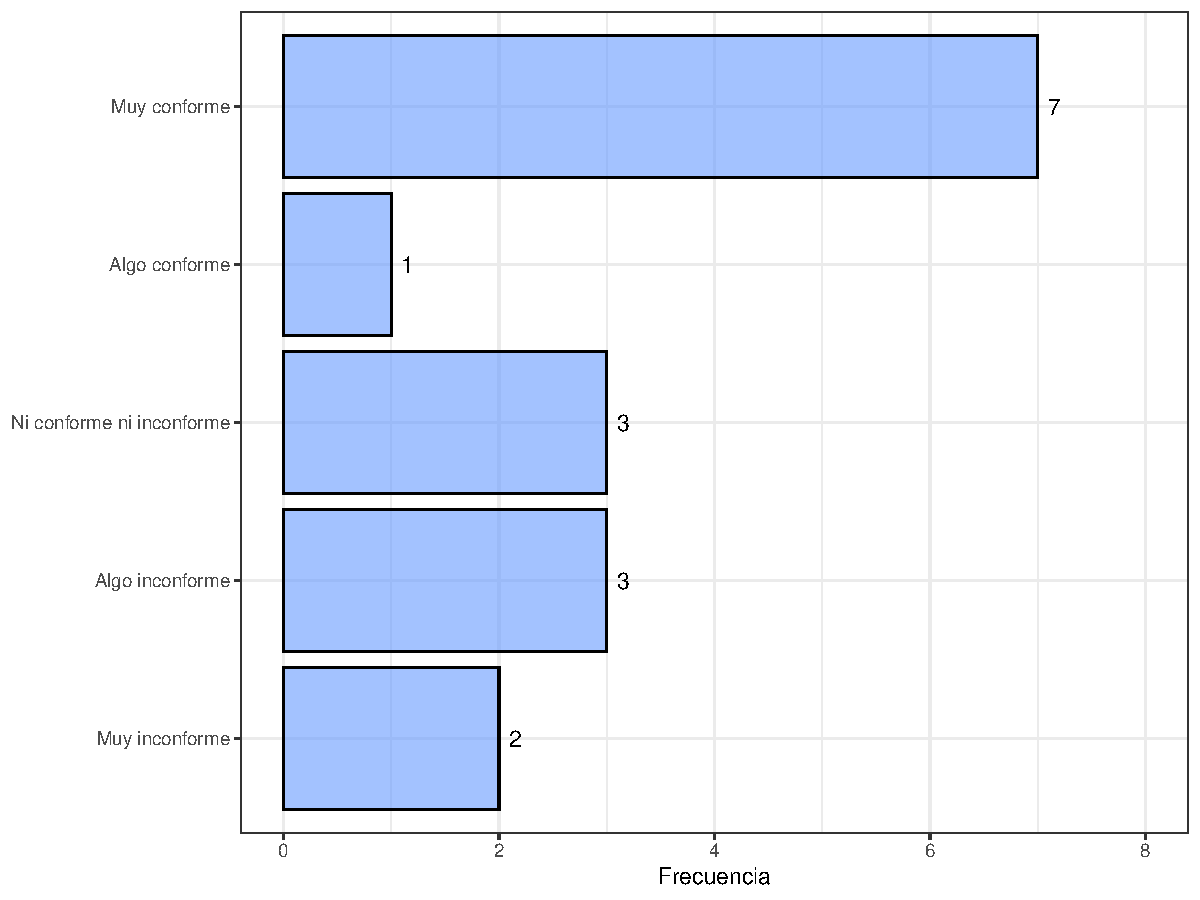
\includegraphics[width=1\linewidth]{InformeFinal_files/figure-latex/ColombiaCompra-1} 

}

\caption{Opinión sobre la plataforma Colombia Compra Eficiente.}\label{fig:ColombiaCompra}
\end{figure}

En algunos casos, los FRE manifestaron la necesidad de recibir capacitación sobre el uso de esta herramienta, pues el desconocimiento sobre la misma por parte del personal puede ocasionar demoras en el proceso de compra de MME. Por ejemplo, como ocurre en el caso del FRE Sucre que si bien tienen un método eficiente para realizar la estimación de compra, se ve retrasado en la etapa que implica el uso de esta plataforma.

Si bien la plataforma Colombia Compra Eficiente buscan hacer más eficiente el proceso de adquisición de bienes y servicios para entidades estatales se observa que en algunos territorios no hay adherencia al uso de la plataforma por desconocimiento de esta. Se recomienda que los FRE fortalezcan el conocimiento de uso de la plataforma.

\hypertarget{recepciuxf3n-de-medicamentos}{%
\subsection{Recepción de medicamentos}\label{recepciuxf3n-de-medicamentos}}

A nivel nacional se cuenta con el \emph{``Manual de condiciones esenciales y procedimientos del Servicio Farmacéutico''} que está determinado por la Resolución 1403 del 2007\textsuperscript{\protect\hyperlink{ref-MinisteriodeSaludyProteccionSocial2007}{34}} emitida por el INVIMA, que en el título ``Recepción y Almacenamiento de Medicamentos y Dispositivos Médicos'', establece que la persona encargada de recibir los medicamentos en la institución debe realizar el siguiente procedimiento:

\begin{enumerate}
\def\labelenumi{\arabic{enumi}.}
\item
  estudiar la documentación propia de la institución que realiza la recepción, con el fin de establecer los productos a recibir y qué condiciones requieren los mismos para su recepción.
\item
  verificar la documentación de quien hace la entrega, p.ej. guía de entrega. Las cantidades solicitadas deben corresponder con las aprobadas tras el pedido.
\item
  realizar una inspección de los medicamentos para verificar las (i) unidades, (ii) número de lote, (iii) fechas de vencimiento, (iv) registro sanitario, (v) laboratorio fabricante, (vi) condiciones de almacenamiento durante el transporte, (vii) manipulación, (viii) embalaje, (ix) material de empaque / envase y (x) condiciones administrativas y técnicas establecidas en la negociación.
\end{enumerate}

Después de la inspección, se realiza un muestreo para determinar si los productos recibidos cumplen con especificaciones de calidad. Existen planes de muestreo de aceptación por atributos en el que se suele utilizar la Tabla Militar Estándar MIL-STD-105E\textsuperscript{\protect\hyperlink{ref-AmericanNationalStandardsInstitute2013}{40},\protect\hyperlink{ref-GutierrezPulido2008}{41}}, con el fin de seleccionar el tamaño de una muestra aleatoria de acuerdo al tamaño total del pedido, nivel de inspección requerido y otros factores. En casos con un tamaño total de lote pequeño y altos niveles de inspección se suele realiza una inspección completa de los productos recibidos.

Al terminar la inspección se pasa a documentar la recepción y se procede a realizar un ``acta de recepción'' donde se detalla la información del procedimiento como:

\begin{itemize}
\item
  fecha y hora de entrega
\item
  cantidad de unidades
\item
  número de lote
\item
  registro sanitario
\item
  fechas de vencimiento
\item
  condiciones de trasporte, manipulación y embalaje
\item
  material de empaque y envase
\item
  condiciones administrativas y técnicas establecidas en la negociación así como la trazabilidad
\end{itemize}

El acta es firmada por las persona que reciben y entregan para ser archivada. Como parte final se ingresan como parte del inventario a todos los productos pedidos que cumplan con las especificaciones de calidad.

En el caso de los distintos FRE a nivel nacional (ver Figura \ref{fig:TiemposRecepcionAlmacenamientob}), se observa que el FRE Antioquia es el que más días invierte en realizar el proceso de recepción, esto se debe a que sus pedidos son de gran tamaño para cubrir la demanda, lo que conlleva a que deba dispensarse 5 días en todo el proceso de recepción técnica, desde el momento de recepción del producto proveniente del FNE, hasta el ingreso de la misma al sistema, incluyendo la realización del acta.

\begin{figure}

{\centering 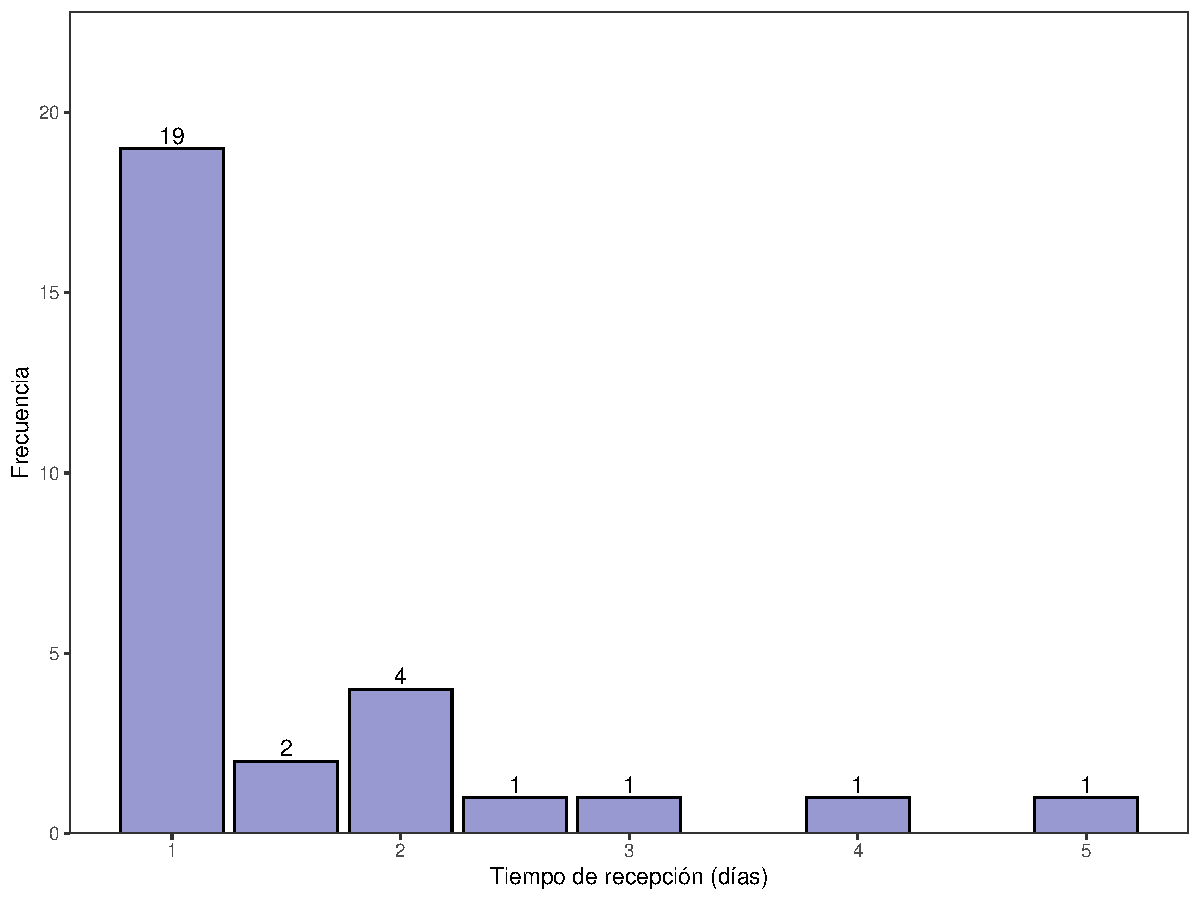
\includegraphics[width=1\linewidth]{InformeFinal_files/figure-latex/TiemposRecepcionAlmacenamientob-1} 

}

\caption{Tiempos en la recepción técnica y almacenamiento de MME. (A) Gráfico de barras con frecuencia. (B) Mapa con tiempos para la recepción técnica de MME.}\label{fig:TiemposRecepcionAlmacenamientob}
\end{figure}

En segundo lugar se encuentra el FRE Boyacá, el cual presenta un uso de 3 días en todo el proceso, se observa que el volumen de inscritos es alto y que en este caso lo llevan dos regentes de farmacia dando paso a la realización de acta con el transportador y luego una revisión completa de cada medicamentos y correcto almacenamiento con su acta correspondiente.

Como otro atributo que se puede resaltar en la Figura \ref{fig:TiemposRecepcionAlmacenamientob}, es que cinco territorios Atlántico, Quindío, Sucre, Tolima y Bolívar se demoran entre 2-2.5 días para la recepción técnica, debido a su tamaño y a la cantidad de personas disponibles para llevar a cabo este proceso y como ultima observación, se puede ver que 24 de los 31 FRE realizan la recepción técnica durante un día y por máximo un día y medio, debido a que los pedidos realizados no son muy grandes, o como en el caso del Valle del cauca, Cauca y Santander, que son territorios grandes con bastantes inscritos, se determina la prioridad de esta acción donde se establece las personas que llevan a cabo este procedimiento y se ha observado que no sobrepasa un día y medio en esta labor.

\hypertarget{traslados-interdepartamentales}{%
\subsection{Traslados interdepartamentales}\label{traslados-interdepartamentales}}

La cadena de suministro de MME está planteada de manera que los FRE realizan compras de MME al FNE, y los establecimientos en los departamentos realizan compras al FRE, en ambos casos sin intermediaciones\textsuperscript{\protect\hyperlink{ref-MSPS1478-2006}{1}}. Sin embargo, existe un mecanismo conocido como \textbf{traslado interdepartamental} mediante el cual un departamento puede realizar la compra de MME a otro departamento. En logística, se le conoce a este tipo de transacciones como \textbf{transbordos laterales}\textsuperscript{\protect\hyperlink{ref-Silver2017}{29}}.

Los traslado interdepartamental/transbordos laterales en su modalidad reactiva se utilizan cuando existe un riesgo de desabastecimiento inminente y se hace un pedido de medicamentos al FRE de un departamento cercano\textsuperscript{\protect\hyperlink{ref-Paterson2011}{42}}, esto puede reducir los costos sí se utiliza en emergencias, o aumentarlos sí se utiliza de forma excesiva\textsuperscript{\protect\hyperlink{ref-Silver2017}{29}}. Es importante mencionar que los traslados interdepartamentales sólo se pueden llevar a cabo previa autorización del FNE.

En el traslado interdepartamental de medicamentos se observa que los territorios más descentralizados son los que presentan mayor demora para recibir los traslados de MME, siendo los casos más demorados San Andrés y Amazonas. Como se observa en la Figura \ref{fig:TiemposTranslados} las regiones más afectadas son Amazonía, Orinoquía, Pacífico a excepción del Valle del Cauca y algunos departamentos del Caribe. Sin embargo, el departamento que más demora presenta es San Andrés, pues al estar alejado de la zona continental del país, tiene un tiempo de traslado de medicamentos más largo.

\begin{figure}[t]

{\centering 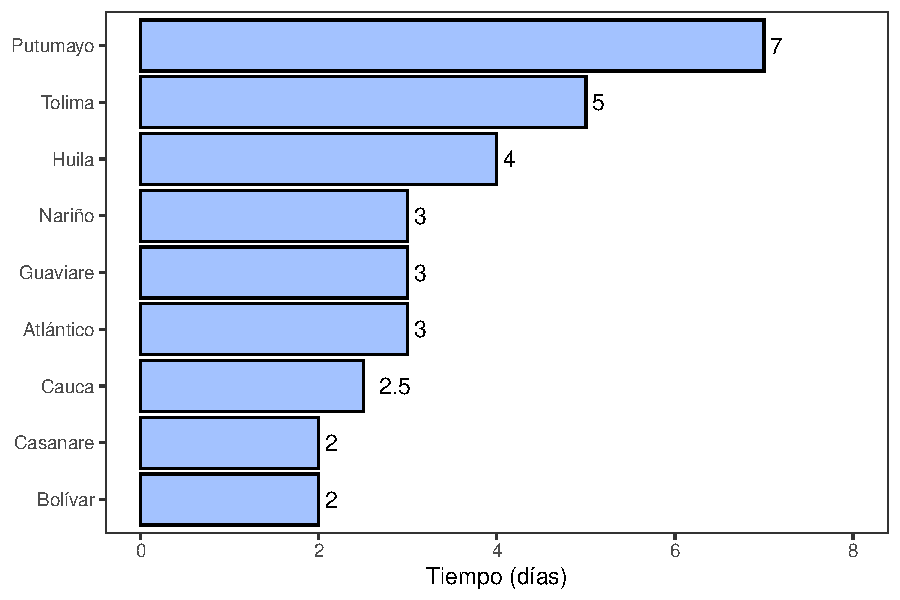
\includegraphics[width=1\linewidth]{InformeFinal_files/figure-latex/TiemposTranslados-1} 

}

\caption{Caracterización en demoras de traslados interdepartamentales. (A) Gráfico de tiempos de traslados interdepartamentales reportados para los departamentos. (B) Mapa de tiempos de traslados interdepartamentales.}\label{fig:TiemposTranslados}
\end{figure}

\hypertarget{venta-de-mme}{%
\section{Venta de MME}\label{venta-de-mme}}

\maxdeadcycles=1000

La venta de MME a instituciones en los departamentos se da según lo establecido por cada FRE y las necesidades de cada departamento, p.ej. en el departamento de Vaupés cuyo abastecimiento se enfoca en satisfacer la demanda del Hospital, no se realiza venta a otras IPS y por lo tanto ni si quiera tienen necesidad de almacenar los medicamentos en el FRE, las compras se destinan inmediatamente al Hospital. Se presenta un caso diferente en departamentos con mayor población y necesidad de medicamentos como Risaralda donde la venta de MME es frecuente, sin embargo, se ha establecido a las IPS que deben proyectar sus necesidades mensualmente.

\begin{figure}[t]

{\centering 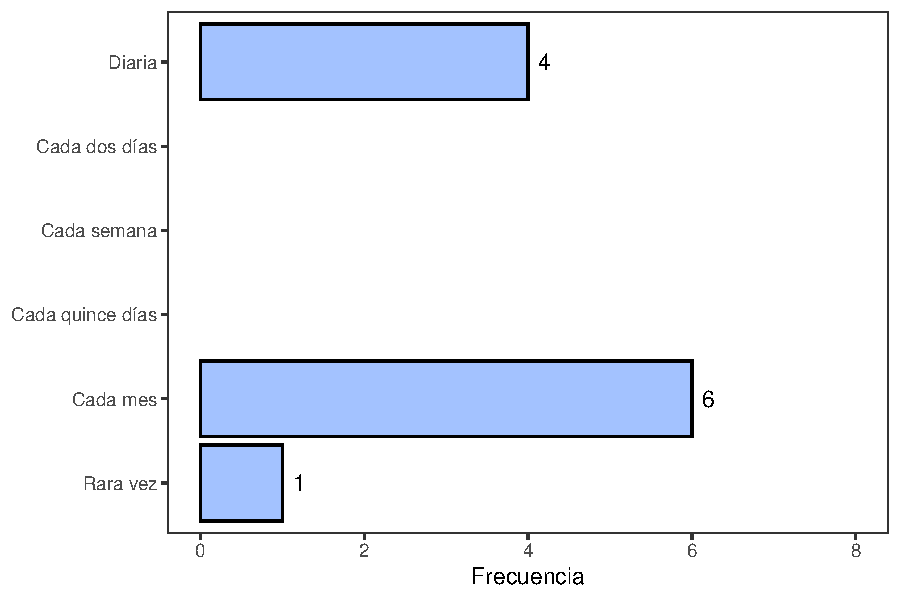
\includegraphics[width=0.85\linewidth]{InformeFinal_files/figure-latex/FrecVentaInstituciones-1} 

}

\caption{Frecuencia de venta de MME a instituciones en el departamento.}\label{fig:FrecVentaInstituciones}
\end{figure}

En el departamento del Atlántico antes de la pandemia la venta de medicamentos se hacía diariamente, sin embargo, por la contingencia en salud se decidió que solo se despachan medicamentos dos días a la semana. Otro departamento que hace venta diaria de MME es Choco y afirma que las necesidades de MME pueden variar en el departamento gracias al traslado no esperado de pacientes de zonas muy distantes a las capitales de los departamentos de Antioquia y Valle del Cauca.

\hypertarget{controles-en-venta-directa-a-paciente}{%
\subsection{Controles en Venta Directa a Paciente}\label{controles-en-venta-directa-a-paciente}}

En la Figura \ref{fig:ControlesVentasFRE} se tienen las medidas adoptadas como controles en la venta directa de MME a pacientes. La más común es la revisión exhaustiva del recetario (realizada por 22 de 30 FRE), seguido de la solicitud de identificación a los pacientes (realizada por 21 de 30 FRE). Existen otras medidas aplicadas como revisión de registro del prescriptor, revisión de historias clínicas y llamada al médico prescriptor. Por último, existen medidas menos poco frecuentes como visitas domiciliarias, llamadas al servicio farmacéutico, llamada al paciente o posposición de la entrega. Se tienen algunos FRE que no realizan controles, debido a que no realizan dispensación a los pacientes como Quindío, Valle del Cauca, Putumayo, Nariño o Risaralda.

\begin{figure}[t]

{\centering 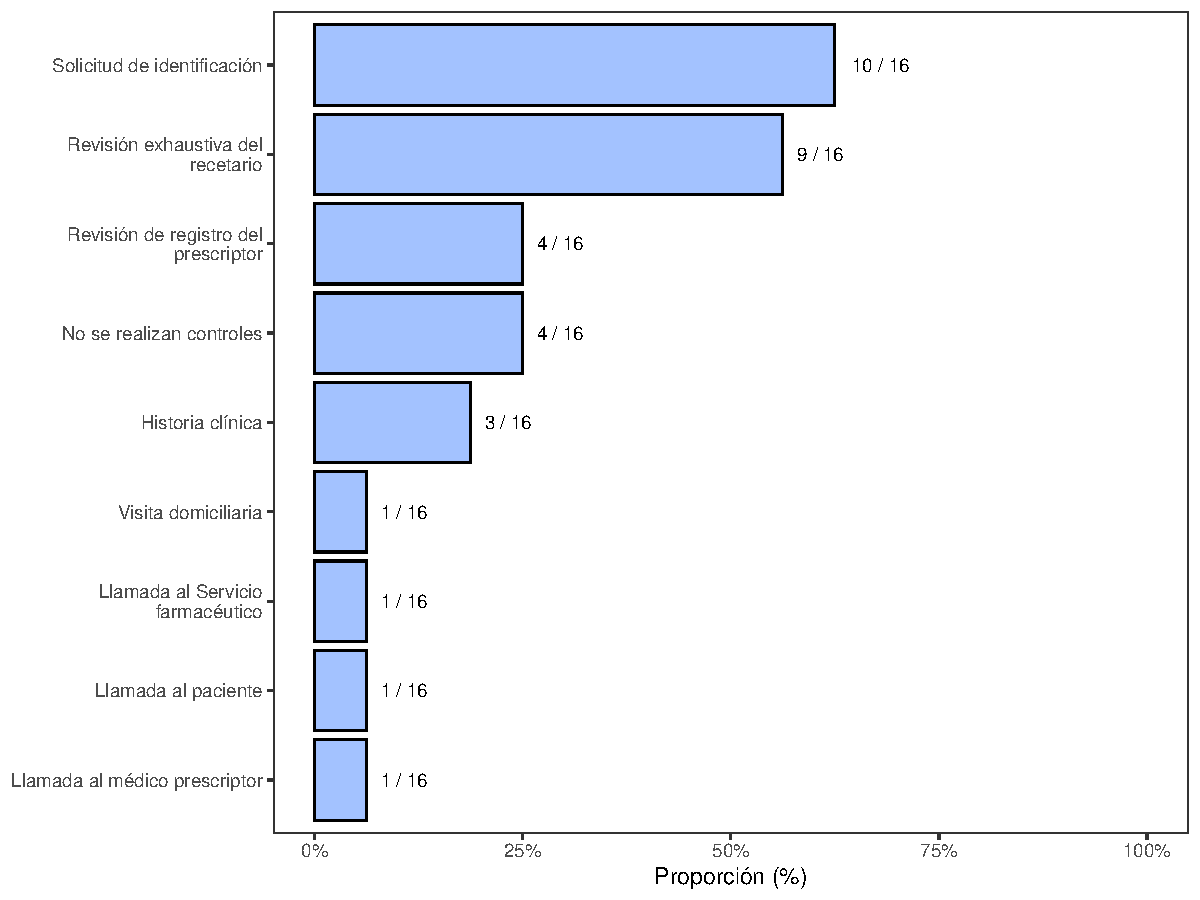
\includegraphics[width=0.85\linewidth]{InformeFinal_files/figure-latex/ControlesVentasFRE-1} 

}

\caption{Controles en las ventas directas a pacientes.}\label{fig:ControlesVentasFRE}
\end{figure}

En la Figura \ref{fig:InstitucionesAdicionales} se muestra sí en el departamento existen otras instituciones que realicen ventas de MME a instituciones a parte del FRE. Se observa que len la mayoría de departamentos sólo el FRE vende MME, la venta por parte de otras instituciones ocurre en los departamentos de Antioquía, Atlántico, Santander, Caldas, Quindío, Nariño, y San Andrés, Providencia y Santa Catalina. La mayoría de los establecimientos autorizados son mayoristas, aunque en algunos casos estos establecimientos tienen autorización para cubrir horarios en que el FRE no se encuentra activo.

\begin{figure}

{\centering 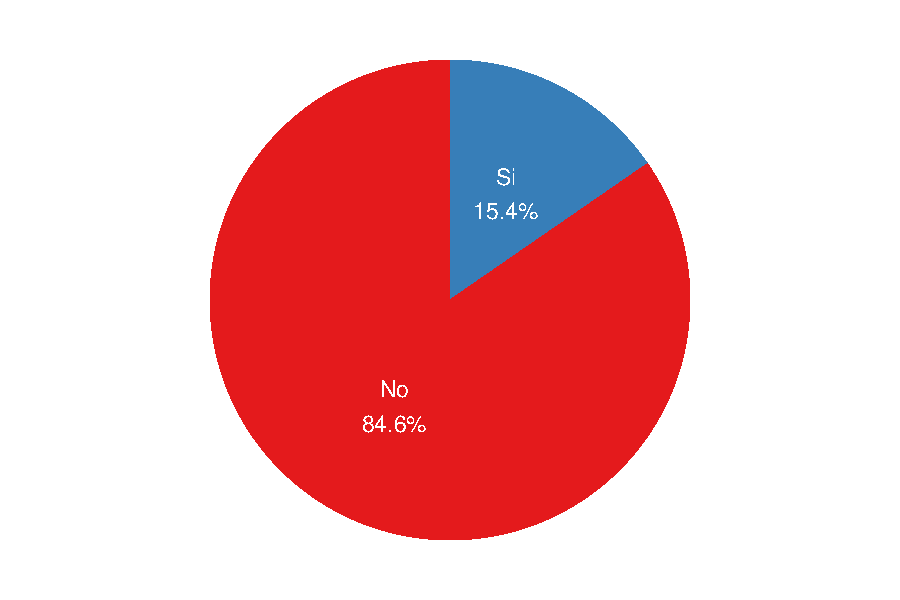
\includegraphics[width=0.85\linewidth]{InformeFinal_files/figure-latex/InstitucionesAdicionales-1} 

}

\caption{Existencia de otras instituciones que realizan ventas a instituciones a MME.}\label{fig:InstitucionesAdicionales}
\end{figure}

\hypertarget{almacenamiento}{%
\section{Almacenamiento}\label{almacenamiento}}

\hypertarget{medidas-de-seguridad-para-el-almacenamiento}{%
\subsection{Medidas de seguridad para el almacenamiento}\label{medidas-de-seguridad-para-el-almacenamiento}}

\maxdeadcycles=1000

En la Figura \ref{fig:MedidasSeguridadAlmacenamientoMME} se listan las medidas de seguridad adoptadas por los FRE para disminuir la posibilidad de robo con fines de desvío de los MME. Las medidas más adoptadas por parte de los FRE consisten en: (i) el acceso de seguridad restringido a cierto personal (con respuesta afirmativa por parte de 18 de 26 FRE), seguido de (ii) gabinetes con llaves simple (en 14 de 26 FRE), (iii) almacenamiento en oficina privada (14 de 26 FRE responden que lo aplican), (iv) inventarios físicos diarios, y (v) protección en gabinetes hechos de materiales resistentes.

\begin{figure}[!t]

{\centering 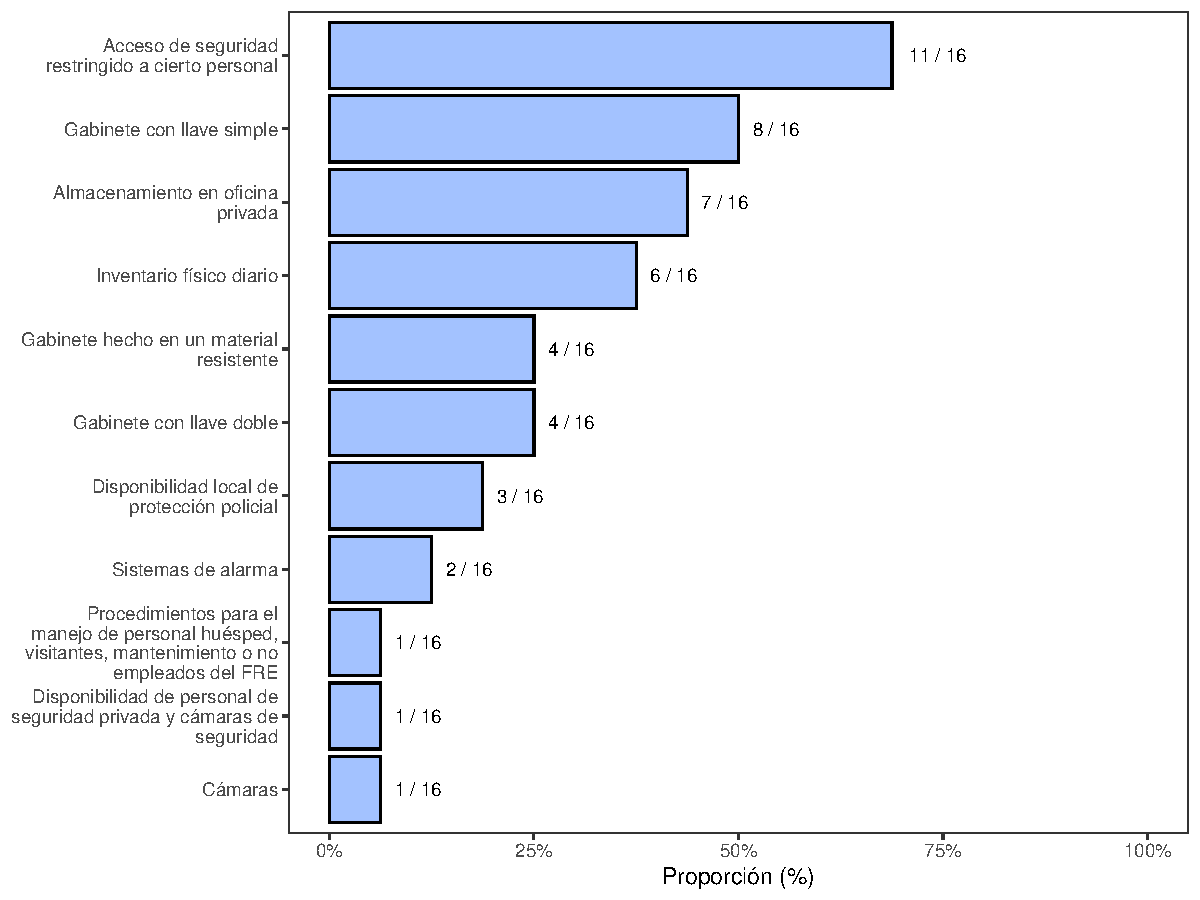
\includegraphics[width=0.95\linewidth]{InformeFinal_files/figure-latex/MedidasSeguridadAlmacenamientoMME-1} 

}

\caption{Medidas de seguridad en el almacenamiento de MME.}\label{fig:MedidasSeguridadAlmacenamientoMME}
\end{figure}

El departamento que reporta la mayor cantidad de medidas de seguridad es César con 7 medidas como: (i) acceso de seguridad restringido a cierto personal, (ii) procedimientos para el manejo de personal huésped, (iii) visitantes, (iv) mantenimiento o no empleados del FRE, (v) almacenamiento en oficina privada, (vi) inventario físico diario, y (vii) Disponibilidad local de protección policial. Entre los FRE con mayor número de medidas de seguridad reportadas se tiene Casanare (con 6 medidas reportadas), y Córdoba, Antioquia, Norte de Santander, Valle del Cauca, Guaviare y Risaralda con 5 medidas reportadas. Los FRE de Atlántico, Magdalena, Huila, Quindío, y Amazonas sólo reportan una medida de seguridad.

Sólo los FRE de Valle del Cauca y Córdoba reportan la existencia de un sistema de monitoreo por cámaras para los medicamentos. Sólo los FRE de Córdoba y Vichada reportan la presencia de seguridad privada como medida de seguridad para los FRE. Se recomienda la adopción de una o varias medidas de seguridad por parte de los FRE frente a posibles robos con intenciones de desvío o tráfico de medicamentos MME.

\hypertarget{revisiuxf3n-de-condiciones-ambientales}{%
\subsection{Revisión de condiciones ambientales}\label{revisiuxf3n-de-condiciones-ambientales}}

En la Figura \ref{fig:FrecRevCondiciones} se muestra la frecuencia de revisión de condiciones ambientales en el almacenamiento de MME. Se tienen que la práctica más frecuente en los FRE es la realización de verificación de condiciones ambientales por lo menos dos veces al día. Sólo algunos FRE afirman que no hacen revisión de condiciones ambientales como Bolívar, Sucre, Chocó, Norte de Santander, Amazonas y Vichada.

\begin{figure}[!b]

{\centering 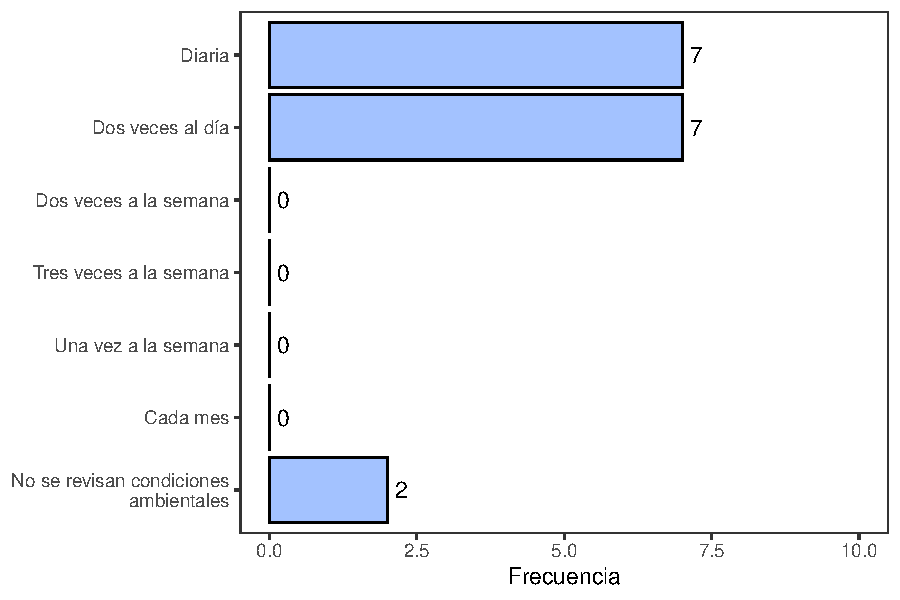
\includegraphics[width=0.9\linewidth]{InformeFinal_files/figure-latex/FrecRevCondiciones-1} 

}

\caption{Frecuencia de revisión de condiciones ambientales.}\label{fig:FrecRevCondiciones}
\end{figure}

En el panel izquierdo de la Figura \ref{fig:MetodosSeguimientoControlAmbiental} se presentan los métodos o tecnologías utilizadas en la monitorización de los medicamentos. En la Figura \ref{fig:MetodosSeguimientoControlAmbiental} se observa que al menos 25 de 30 fondos rotatorios cuentan con un termohigrómetro para la evaluación de condiciones ambientales. La práctica de diligenciar registros cuenta con una menor adopción por parte de los fondos rotatorios, se tiene que 7 y 4 de los fondos rotatorios realiza el diligenciamiento de estos formatos de manera manual y electrónica de manera respectiva.

\begin{figure}[t]

{\centering \includegraphics[width=1\linewidth]{InformeFinal_files/figure-latex/MetodosSeguimientoControlAmbiental-1} 

}

\caption{(A) Tecnologías de control y seguimiento de condiciones ambientales y (B) Frecuencia de calibración y mantenimiento de equipos de seguimiento ambiental.}\label{fig:MetodosSeguimientoControlAmbiental}
\end{figure}

En sólo dos FRE (Chocó y Norte de Santander) se reporta el uso de aire acondicionado como una medida para el seguimiento de condiciones ambientales. En el panel derecho de la Figura \ref{fig:MetodosSeguimientoControlAmbiental} se tiene que la práctica más común es realizar la calibración de los equipos de monitoreo por lo menos una vez al año, y hasta en 11 se tiene que no hay un procedimiento de calibración de los equipos. La mayoría de departamentos que no realizan el proceso de calibración se encuentran en la región central.

\hypertarget{espacio-de-almacenamiento}{%
\subsection{Espacio de almacenamiento}\label{espacio-de-almacenamiento}}

En la Figura \ref{fig:ProductosCompartidos1} se muestra la frecuencia de varias categorías de productos con los cuales se comparten los MME en el almacén de los FRE. Se tiene que en casi la mitad de los FRE se comparten los MME con medicamentos de salud pública, en 7 de 30 casos se reporta la utilización del espacio en conjunto con papelería (7/30) o recetarios oficiales (3/30). Algunos FRE tienen otros items como vacunas, medicamentos de carros de paro y medicamentos incautados. En 9 de 30 casos se tiene que el FRE tiene un espacio dedicado únicamente a MME.

\begin{figure}

{\centering \includegraphics[width=0.85\linewidth]{InformeFinal_files/figure-latex/ProductosCompartidos1-1} 

}

\caption{Productos compartidos en el almacén de MME.}\label{fig:ProductosCompartidos1}
\end{figure}

En la Figura \ref{fig:PropOcupacionAlmacen} se tiene una estimación del promedio de ocupación de medicamentos MME en los almacenes frente a otros productos. Se tiene que la práctica más común es la utilización de un espacio destinado exclusivo para estos medicamentos y esto se da en 12 FREs.

\begin{figure}

{\centering \includegraphics[width=0.85\linewidth]{InformeFinal_files/figure-latex/PropOcupacionAlmacen-1} 

}

\caption{Ocupación promedio del MME frente a otros medicamentos o ítems almacenados en el FRE.}\label{fig:PropOcupacionAlmacen}
\end{figure}

Se considera que existen dos tipos de métodos de control de inventario conocidos como sistemas perpetuos o periódicos\textsuperscript{\protect\hyperlink{ref-Silver2017}{29}}.
En la Figura \ref{fig:FrecControlExistencias} se tiene una caracterización de la frecuencia de control de existencias de los MME. En la mayoría de los FRE se realiza esta verificación de manera mensual, o de forma diaria. La frecuencia de monitoreo de existencias parece estar relacionada con el nivel medio de inventario.

\begin{figure}

{\centering \includegraphics[width=1\linewidth]{InformeFinal_files/figure-latex/FrecControlExistencias-1} 

}

\caption{Frecuencia del control de existencias de medicamentos MME.}\label{fig:FrecControlExistencias}
\end{figure}

Entre los FRE que afirman realizar el monitoreo de niveles de inventarios de forma diaria se encuentran Antioquia, Córdoba, Bolívar, San Andrés, Casanare, Meta y Caldas. El FRE de Cesar afirma realizar el control de existencias varias veces al día. Los FRE que realizan monitoreo cada mes parecen encontrarse en las regiones más periféricas del territorio, y esto se podría deber a la presencia de niveles de inventario promedio bajos.

\hypertarget{control-de-fechas-de-vencimiento}{%
\subsection{Control de fechas de vencimiento}\label{control-de-fechas-de-vencimiento}}

De acuerdo a la Resolución 1403 de 2007 del MSPS\textsuperscript{\protect\hyperlink{ref-MinisteriodeSaludyProteccionSocial2007}{34}}, el control de fechas de vencimiento es un procedimiento importante enmarcado en el proceso de Recepción y Almacenamiento de Medicamentos y Dispositivos Médicos dentro del Modelo de Gestión del Servicio Farmacéutico. Los servicios farmacéuticos deben contar con criterios procedimientos y recursos que le permitan verificar y recursos que permitan verificar continuamente la fecha de vencimiento de los medicamentos\textsuperscript{\protect\hyperlink{ref-MinisteriodeSaludyProteccionSocial2007}{34}}.

Entre estos recursos se encuentra la \emph{semaforización}, que es una herramienta que permite identificar y determinar en el momento oportuno que medicamentos están próximos a vencer. De forma común, esta herramienta se aplica mediante la rotulación de las unidades con colores de los medicamentos de acuerdo al tiempo esperado hasta la fecha de vencimiento\textsuperscript{\protect\hyperlink{ref-HernandezVera2017}{43}}. La semaforización también se podría aplicar mediante sistemas de alertas electrónica.

La adopción de esta práctica sólo se ha realizado en 40\% de los FRE. Esta práctica se lleva a cabo teniendo en cuenta tres colores:

\begin{itemize}
\item
  Rojo: medicamento que se encuentra próximo a vencer.
\item
  Amarillo: medicamento que se encuentra en riesgo moderado de vencimiento.
\item
  Verde: medicamento que no tiene riesgo de vencimiento. En ocasiones, no se genera ningún tipo de alerta cuando el producto está en esta condición.
\end{itemize}

Los umbrales adoptados por la mayoría de las entidades ha sido \texttt{6\textbar{}12} que indica colocar una etiqueta roja sí el medicamento se encuentra a 6 meses de vencerse, y una etiqueta amarilla sí el medicamento se encuentra a 12 meses de vencerse. Algunos FRE también tienen umbrales de \texttt{3\textbar{}6} meses para el proceso de semaforización.

En la Figura \ref{fig:CasosVencimiento1}A se observa que el 71\% de los FRE han presentado casos de medicamentos vencidos lo que constituye a 22 de 31 FRE existentes en el país, y esto indica que los vencimientos son una situación frecuente para los FRE. En la Figura \ref{fig:CasosVencimiento1}B se muestran los medicamentos más involucrados en casos de vencimientos. En primer lugar, se tiene al Metilfenidato Tableta x 10 mg ya que 13 de los 31 FRE han presentado vencimientos relacionados a este producto. La razón para estos vencimientos podría deberse a varios factores como:

\begin{itemize}
\item
  El producto cuenta con una vida útil de 18 meses.
\item
  Este medicamento es importado y en ocasiones la casa matriz entrega el producto con una vida útil efectiva menor a los 18 meses mencionados.
\item
  Debido a la emergencia sanitaria producida por el coronavirus se ha presentado una contracción importante de la demanda que se encuentra posiblemente relacionada a los cambios en la movilidad de los ciudadanos y las restricciones de presencialidad en instituciones escolares.
\end{itemize}

El segundo medicamento más involucrado en casos de vencimiento es Primidona Tableta x 250 mg debido a que 4 de los 31 FRE reportan casos de vencimientos, seguido de los vencimientos de Meperidina de 100mg/2mL, Fenobarbital Solución inyectable x 40 mg/mL y Fenobarbital Solución inyectable x 200 mg/mL que fueron reportados por 3 de 31 FREs a nivel nacional que se puede explicar debido a que son productos de baja rotación, y es posible que los FRE no hayan recibido una adecuada asistencia por parte del FNE para el manejo de ítems de este tipo.

\begin{figure}[t]

{\centering \includegraphics[width=1\linewidth]{InformeFinal_files/figure-latex/CasosVencimiento1-1} 

}

\caption{Vencimiento de medicamentos. (A) Presentación de casos de vencimiento de MME. (B) Medicamentos implicados en casos de vencimiento de MME.}\label{fig:CasosVencimiento1}
\end{figure}

\hypertarget{transporte}{%
\section{Transporte}\label{transporte}}

El transporte de medicamentos por parte del FNE, es un proceso importante dentro de la cadena de suministro de MME. Los costos de transporte de medicamentos por parte del FNE están cubiertos dentro del precio de los MME, para la distribución mediante el canal FRE. El FNE contrata a una empresa especializada en distribución logística de mercancías y bienes para la entrega del producto a nivel nacional.

En la Figura \ref{fig:TransporteProductos} se tiene una descripción de la opinión del servicio de distribución por parte del FNE. Se tiene que las opiniones se encuentran divididas con algunas respuestas positivas (66.6\%) y otras negativas (33.3\%).

\begin{figure}

{\centering \includegraphics[width=1\linewidth]{InformeFinal_files/figure-latex/TransporteProductos-1} 

}

\caption{Opinión del servicio de la distribución de los medicamentos MME.}\label{fig:TransporteProductos}
\end{figure}

En cuanto a las opiniones negativas se tiene como principal queja a las averías en los productos causadas por el transporte. Se tienen también quejas relacionadas con (i) problemas en el enrutamiento de los envíos, (ii) demoras, (iii) disposición de los medicamentos en la entrada de las secretarías sin entregarlos de forma directa a los encargados, (iv) falta de cobertura en todo el territorio y (v) condiciones de almacenamiento inadecuadas.

\begin{quote}
\emph{``Problemas de embalaje y muchos problemas de averías''}
\end{quote}

Los problemas en el transporte de medicamentos han generado inconvenientes relacionados a sobrecostos en este mismo rubro, de manera que algunos FRE han tenido que recurrir a otros convenios, por ejemplo como aquellos utilizados por medicamentos de salud pública.

En cuanto a las respuestas positivas se tiene que la mayoría de los FRE que responden de esta manera no han tenido inconvenientes con la entrega de los productos. Algunos de estos FRE manifiestan que la empresa hace llegar el producto dentro de 5 días después del despacho, así mismo que los medicamentos llegan en buenas condiciones y que no se han tenido problemas. Sólo algunos de los FRE no tienen registros de inconvenientes con el transportador previamente. Un ejemplo de respuesta positiva ha sido:

\begin{quote}
\emph{``No hemos tenido inconvenientes con el transporte de MME. Cuando surge un caso de producto no conforme, el FNE siempre responde y efectúa la devolución de estos productos con averías.''}
\end{quote}

Se tiene que pese a que más del 50\% de los respondientes de la encuesta tienen una opinión positiva del transporte de los medicamentos, casi 1 de cada 3 FRE no están satisfechos con el servicio. El alto grado de insatisfacción y las causas que justifican la opinión se deben tener en cuenta como aspectos para el mejoramiento del proceso.

\hypertarget{precioMedicamentos}{%
\section{Precio de medicamentos}\label{precioMedicamentos}}

\maxdeadcycles=1000

El gasto farmacéutico es una parte importante del gasto público en salud, y por esto se vuelve importante su control. Por otra parte, la definición de los precios de los medicamentos genera tensiones entre la libertad económica de los laboratorios, distribuidores y comercializadores de medicamentos frente al derecho a la salud de los pacientes que requieren de los beneficios de las tecnologías en salud\textsuperscript{\protect\hyperlink{ref-AvilaRoncancio2019}{44}}.

En Colombia se ha establecido un modelo de regulación de precios de medicamentos por lo cual existen tres regímenes de regulación: (i) Libertad regulada, (ii) Libertad vigilada y (iii) Control directo\textsuperscript{\protect\hyperlink{ref-CongresodelaRepublicadeColombia1988}{45}}. De estos se tiene que la Comisión Nacional de Precios de Medicamentos y Dispositivos Médicos (CNPMDM) sólo utiliza la Libertad Vigilada y el Control Directo\textsuperscript{\protect\hyperlink{ref-SecretariaTecnicaCNPDM-2019}{46}}.

De acuerdo al ABC de la Regulación de Precios de Medicamentos, se ha observado un margen entre el precio ex-fábrica y el precio de distribuidor de aproximadamente el 7\% teniendo en cuenta los datos internacionales, y se sugiere este márgen para referencia en el mercado colombiano\textsuperscript{\protect\hyperlink{ref-SecretariaTecnicaCNPDM-2019}{46}}.

En la gestión de operaciones de distribución de MME por parte del FNE, se consideran dos canales de distribución principales los cuales son: (i) canal de distribución a FRE y (ii) canal de distribución mediante compra directa. Se considera que el canal de compra directa constituye una excepción, en los casos en donde no existe un Fondo Rotatorio que realice la distribución en un departamento determinado. Debido a esto, se debe considerar un precio de venta mayor en la utilización del canal de compra directa. En el caso de MME se realiza la estimación del precio de venta a FRE y se adiciona un margen del 12\% para las operaciones en canal de compra directa.

En la Figura \ref{fig:precioVentasDepartamentos} se observa una comparación de los precios de ventas reportados como oficiales por los FRE en sus respectivos departamentos para la vigencia 2021. El precio se muestra para cada medicamento en una escala de color diferente en pesos colombianos. En la Figura \ref{fig:precioVentasDepartamentos} se puede observar que los medicamentos más costosos corresponden a Metilfenidato 36 mg (entre \(\$300.000\) y \(\$900.000\)) y Metilfenidato 36 mg (entre \(\$200.000\) y \(\$600.000\) pesos).

\begin{figure}[t!]
\includegraphics[width=1\linewidth]{InformeFinal_files/figure-latex/precioVentasDepartamentos-1} \caption{Precio de venta de medicamentos en los FRE.}\label{fig:precioVentasDepartamentos}
\end{figure}

En la línea de anticonvulsivantes se tiene que el medicamento más costoso es Fenobarbital 200 mg/mL con precios entre \(\$75.000\) a \(\$150.000\), mientras que en la línea de narcóticos se tiene al producto importado de Metadona tabletas 40mg como el más costoso (con precios que rondan \(\$100.000\) y \(\$200.000\)). Se tiene algunos departamentos con un color gris, lo que indicaría que el medicamento no hace parte del portafolio de MME que es distribuido en el departamento. Por otra parte, se tienen departamentos con un color de relleno blanco lo que indicaría casos en los que no se presenta un reporte activo de los precios de ventas en esos departamentos, se tienen como casos a Bolívar, Risaralda, Meta, Vichada, y Guainía.

Se realizó una comparación de márgenes de precios de venta frente a los precio de compra de MME por parte de los FRE, se tiene como referencia a los precios indicados en la plataforma de compra eficiente.

\[\mathrm{M}~(\%) = \frac{p}{v} \cdot 100\%\]

Donde, \(\mathrm{M}\) es el márgen de beneficio sobre el costo de adquisición \(v\) por parte del FRE (precio de venta del FNE), y \(p\) es el precio de venta desde el FRE. En el panel A de la Figura \ref{fig:boxplotComparativoPVTA} se tiene una comparación de los márgenes de precio de venta frente a precio de compra de los MME. En verde, se tienen los medicamentos con una mediana de precios de ventas en departamentos menor al margen de venta mediante el canal de compra directa correspondiente a (112\%), en estos medicamentos se tiene a Morfina solución oral 3\%, Morfina HCl 50mg/mL, Metilfenidato tableta x 36mg, y Meperidina 100mg/2mL (estos medicamentos no tendrían sobrecostos respecto al canal de compra directa).

\begin{figure}[t]
\includegraphics[width=1\linewidth]{InformeFinal_files/figure-latex/boxplotComparativoPVTA-1} \caption{Comparativo de márgenes de precio de venta para: (A) Medicamentos y (B) Departamentos.}\label{fig:boxplotComparativoPVTA}
\end{figure}

En azul se tienen los departamentos con un margen de precios entre 112\% y 120\%, en este casos se constituirían sobrecostos respecto al canal de compra directa para 11 medicamentos. Por último, en rojo se tienen medicamentos con margenes de precios de ventas mayores al 20\% del precio de compra, se tienen los casos de Morfina hcl 10mg/mL, Hidrato de cloral 10\% solución oral y Fenobarbital tabletas x 50mg.

En el panel B de la Figura \ref{fig:boxplotComparativoPVTA} se tienen los márgenes de precio de venta sobre precio de compra de acuerdo a los departamentos, se tienen en verde departamentos con una mediana de márgenes de precio menores al 112\%, en estos departamentos se tiene Atlántico, Córdoba, Boyacá, Tolima, Cauca, Valle del Cauca, Amazonas y Guaviare. En el otro extremo se tienen departamentos que tienen margenes de más del 20\% sobre el precio de compra como Casanare, Sucre, Cesar, La Guajira, Putumayo, Norte de Santander, Chocó, Caquetá, y Arauca.

Por último, se realizó una comparación entre los márgenes de precio de venta en los departamentos y sus distancia física relativa a Bogotá (ver Figura \ref{fig:relacionMargenesCosto}) mediante regresión lineal. Parece existir una relación entre las dos variables, sin embargo la presencia de casos anómalos que se muestran como etiquetas en la figura impiden que se puede establecer una relación con significancia estadística (\(p = .513\)).

También se evaluaron otros factores cómo el número de instituciones que realizaron compras en la vigencia anterior (\(p = .667\)) y la proporción de ingresos constituida por venta de medicamentos (\(p = .429\)) pero no se encontró una relación significativa entre las variables (ver paneles B y C de la Figura \ref{fig:relacionMargenesCosto}.

\begin{figure}[b!]

{\centering \includegraphics[width=0.95\linewidth]{InformeFinal_files/figure-latex/relacionMargenesCosto-1} 

}

\caption{Relación de márgen de ganancia y otras variables. (A) Distancia física en kilómetros, (B) N.° de entidades que realizado compras al FRE durante el último año, y (C) Proporción de ingreso correspondiente a ventas de medicamentos.}\label{fig:relacionMargenesCosto}
\end{figure}

Se debe reconocer que un mal control de precios a nivel de laboratorio y distribuidores puede ocasionar distorsiones importantes en la cadena de suministro de manera que no se produce un beneficio óptimo al considerar toda la cadena. En este caso se podría esperar que precios de venta no competitivos a nivel de FRE generen un aumento en la proporción de compra directa por parte de instituciones en el territorio correspondiente.

Se debe tener en cuenta que un precio de venta alto no siempre garantiza un beneficio neto ya que este depende de la demanda así como las cantidades adquiridas y el nivel de desabastecimiento esperado\textsuperscript{\protect\hyperlink{ref-Silver2017}{29}}. Se deben revisar a profundidad los precios de los medicamentos en el territorio de manera que se articule una política de precios de medicamentos monopolio del Estado.

\hypertarget{ruta-tecnoluxf3gica}{%
\chapter{Ruta Tecnológica}\label{ruta-tecnoluxf3gica}}

\maxdeadcycles=1000

La infraestructura tecnológica de cada FRE es un elemento importante en el avance y cumplimiento de la mayoría de las funciones que tiene como ente territorial. La Figuras \ref{fig:PropHerramientasManejoInventarios} muestra la proporción de herramientas en el manejo de inventarios a nivel nacional y herramientas que usa el FRE para consolidar los informes (Anexos) de la Resolución 1479 de 2006\textsuperscript{\protect\hyperlink{ref-MSPS1479-2006}{2}}. A partir de esta información se detalla el paquete ofimático Microsoft Excel, como la principal herramienta que emplea la mayoría de los FRE departamentales.

\begin{figure}

{\centering \includegraphics[width=0.85\linewidth]{InformeFinal_files/figure-latex/PropHerramientasManejoInventarios-1} 

}

\caption{Proporción de Herramientas en el manejo de inventarios.}\label{fig:PropHerramientasManejoInventarios}
\end{figure}

Así mismo, se encuentran diferentes soportes tecnológicos empleados por el personal de los FRE como Softwares, donde se adelantan estas actividades de inventario y consolidación de informes. Según el panorama, la mayoría de FRE departamentales cuentan con alguna percepción o conocimiento profundo de las herramientas digitales que abarca la infraestructura tecnológica adecuada para el desarrollo de sus principales actividades.

No obstante, se mantiene un grupo numeroso de FRE que permanecen con su gestión manual y evitan la transición de sus procesos manuales a alguna herramienta digital tecnológica. En un mediano futuro, con la implementación del ROE, se deben contemplar estos FRE que se resisten al cambio y eluden su adaptación al mundo digital, en virtud de que el ROE será manejado desde una plataforma tecnológica y el personal del FRE deberá adoptar estos recursos tecnológicos de alguna manera.

Las condiciones en la infraestructura tecnológica de cada FRE, logran evidenciar la capacidad operativa y técnica que tiene el ente territorial, en los procesos internos que realiza referente al manejo de los medicamentos de control especial, la consolidación y envío de informes de la Resolución 1478 de 2006\textsuperscript{\protect\hyperlink{ref-MSPS1478-2006}{1}} y Resolución 1479 de 2006\textsuperscript{\protect\hyperlink{ref-MSPS1479-2006}{2}}. Este componente tecnológico es un elemento crítico para determinar las condiciones actuales de cada FRE. Inicialmente, el canal de comunicación que mantiene el FRE con los usuarios precisa que tan cercano se encuentra el FRE con la población del territorio.

\hypertarget{canales-de-comunicaciuxf3n}{%
\section{Canales de comunicación}\label{canales-de-comunicaciuxf3n}}

De acuerdo con la Figura \ref{fig:MediosComunicacion}, se evidencia que los canales más frecuentes que manejan los FRE para comunicarse con los usuarios corresponden al teléfono y el correo electrónico. Incluso estos medios de comunicación toman mayor relevancia en estos tiempos actuales de distanciamiento social, a causa de la reciente pandemia referente a la COVID-19. En ese orden de ideas, cada vez son menos los FRE que mantienen la atención presencial en sus instalaciones, al igual que la correspondencia. Estos canales de comunicación fueron reemplazados por el mundo moderno y la digitalización, en función del uso correcto del correo electrónico. Este análisis permite demostrar cierta aceptabilidad por los medios digitales que han surgido en la actualidad, por parte del personal del FRE y los usuarios inscritos en el territorio.

\begin{figure}[t!]

{\centering \includegraphics[width=0.9\linewidth]{InformeFinal_files/figure-latex/MediosComunicacion-1} 

}

\caption{Canales de comunicación FRE con clientes.}\label{fig:MediosComunicacion}
\end{figure}

Por otro lado, la Figura \ref{fig:ConexionInternet} exhibe la velocidad de conexión a internet en cada zona del país, donde se encuentran ubicados los FRE de cada departamento. Cerca de la mitad de los FRE cuentan con una concepción ``Buena o excelente'' del internet en su territorio. No obstante, la otra porción equivalente a la mitad de los FRE, afirma una ``Aceptable, mala o muy mala'' señal del internet en su sitio de trabajo. Esto podría representar varios inconvenientes en la conectividad a la red y el desarrollo adecuado de los procesos digitales en muchos FRE departamentales.

La apuesta a futuro de la modernización en los procesos de manejo de recetarios oficiales y MME, por ejemplo, la implementación del ROE, mostraría cierta deficiencia en el acceso a internet para un sector grande en la población colombiana. Esta transformación digital debe considerar principalmente, aquellos territorios que mantienen falencias en la conectividad a internet, con el fin de evitar barreras al acceso de medicamentos en estas zonas del país.

\begin{figure}[b!]

{\centering \includegraphics[width=0.85\linewidth]{InformeFinal_files/figure-latex/ConexionInternet-1} 

}

\caption{Velocidad de conexión de internet.}\label{fig:ConexionInternet}
\end{figure}

\hypertarget{equipos-de-cuxf3mputo}{%
\section{Equipos de cómputo}\label{equipos-de-cuxf3mputo}}

Según la Figura \ref{fig:EquiposComputo}, más de la mitad de los FRE poseen únicamente hasta dos (2) computadores para el desarrollo de sus funciones como ente territorial. En dos casos particulares, FRE Guaviare y FRE San Andrés, no cuentan con equipo de cómputo actualmente y esto influye desfavorablemente en el cumplimiento de sus obligaciones como FRE. En esa misma línea, podemos encontrar nueve FRE que poseen solo un (1) equipo de cómputo, perjudicando igualmente el avance de sus actividades laborales y funciones principales como ente territorial, responsable del control de MME en el departamento. Incluso, según las experiencias y observaciones del personal vinculado a los FRE, disponer de dos (2) computadores sigue siendo una limitante en las herramientas del trabajo, condicionado el adecuado desarrollo laboral. Sin contar que, en la mayoría de departamentos, los equipos de cómputo son insuficientes para el personal del FRE o deben ser cambiados por obsolescencia, según la Figura \ref{fig:OpinionEquiposComputo}.

\begin{figure}

{\centering \includegraphics[width=0.85\linewidth]{InformeFinal_files/figure-latex/EquiposComputo-1} 

}

\caption{N.° de equipos en el FRE.}\label{fig:EquiposComputo}
\end{figure}

Únicamente 6 FRE a nivel nacional, cuentan con cuatro (4) o más computadores en su área de trabajo, cuya índole permite mejores condiciones laborales al personal de apoyo del FRE. Por consiguiente, estos 6 entes territoriales conservan excelentes condiciones de infraestructura tecnológica, cuyo factor facilita la atención de la necesidad de MME en su territorio y favorece en la proyección de la demanda de MME y recetarios oficiales. Si el personal del FRE cuenta con equipos de cómputo suficiente para la gestión apropiada de los MME y los recetarios oficiales, se puede afirmar que estos entes territoriales están sintonizados con la infraestructura tecnológica necesaria para cumplir las funciones de FRE.

Adicionalmente en la Figura \ref{fig:RelacionEquiposPersonal} se presenta la relación entre el requerimiento de equipos y el número de personas en cada FRE. La figura muestra una alta dispersión de los datos y por consiguiente se podría determinar que no hay alguna tendencia permanente entre el número de equipos y el personal vinculado por cada FRE. No obstante, es importante resaltar algunos casos particulares de los FRE que poseen notoriamente más personas vinculadas que equipos de cómputo, correspondiendo a los casos de los FRE Guaviare, Norte de Santander, Boyacá, Guainía, Meta, Risaralda y Tolima. Este factor tecnológico crítico representa gran importancia en estos territorios y se debe prestar mayor atención en la gestión de los MME y recetarios oficiales.

\begin{figure}

{\centering \includegraphics[width=0.85\linewidth]{InformeFinal_files/figure-latex/RelacionEquiposPersonal-1} 

}

\caption{Relación entre el requerimiento de equipos y el número de personas en el FRE.}\label{fig:RelacionEquiposPersonal}
\end{figure}

De acuerdo a la Figura \ref{fig:OpinionEquiposComputo} se puede evidenciar que aproximadamente la mitad de los FRE manifiestan que los equipos de cómputo de la entidad territorial son adecuados para las actividades y funciones del FRE. No obstante, una gran porción de los entes territoriales, mantienen opiniones negativas respecto a su infraestructura tecnológica, cuyo elemento es asociado, en algunos casos, con una negligencia en las actividades internas del FRE por falta de estas herramientas tecnológicas. Como se mencionó anteriormente, la modernización en los procesos referentes al manejo de recetarios oficiales y MME, tendrá que considerar principalmente, aquellos FRE cuyos territorios muestran obstáculos en la disponibilidad tecnológica, representada principalmente por el estado actual de los equipos de cómputo a lo largo del territorio nacional.

\begin{figure}

{\centering \includegraphics[width=0.85\linewidth]{InformeFinal_files/figure-latex/OpinionEquiposComputo-1} 

}

\caption{Opinión sobre los equipos de cómputo del FRE.}\label{fig:OpinionEquiposComputo}
\end{figure}

Si los inconvenientes relacionados a la infraestructura tecnológica, se presentan actualmente en las zonas más alejadas del país, el escenario para la implementación del ROE no podría aspirar a grandes cambios en cada territorio. Lo anterior, podría originar una barrera al acceso de medicamentos desde cada Secretaria de Salud o Dirección departamental de salud. A continuación, se presenta una opinión obtenida durante las visitas técnicas a los FRE:

\begin{quote}
\emph{``Actualmente el FRE \ldots{} está en proceso de cotización y compra de computadores, para las funciones y actividades que debe cumplir el mismo. Se espera contar con 3 equipos de cómputo con funcionalidad completa.''}
\end{quote}

\hypertarget{control-de-la-informaciuxf3n}{%
\section{Control de la información}\label{control-de-la-informaciuxf3n}}

\hypertarget{seguridad-de-la-informaciuxf3n}{%
\subsection{Seguridad de la información}\label{seguridad-de-la-informaciuxf3n}}

La seguridad de la información que manejan los FRE a nivel nacional, es un tema de alta importancia a nivel interno, ya que comprende las medidas preventivas de la institución u organización, que permiten resguardar y proteger la información por medio de sistemas tecnológicos, buscando mantener la confidencialidad, disponibilidad e integridad de los datos. Adicionalmente, se debe contemplar que todos los FRE deben ser capaces de resguardar y proteger la información proveniente de todo el departamento, lo cual dispone un reto mayor referente a la seguridad de la información.

La Figura \ref{fig:GarantiaInformacion} muestra la manera como se garantiza la seguridad de la información en los FRE departamentales. A partir de los datos de la figura, se puede evidenciar que medios emplea el personal del FRE para resguardar y proteger la información por medio de sistemas tecnológicos. La restricción de acceso es el principal recurso que tienen los FRE para mantener la confidencialidad, disponibilidad e integridad de los datos.

\begin{figure}[t!]

{\centering \includegraphics[width=0.95\linewidth]{InformeFinal_files/figure-latex/GarantiaInformacion-1} 

}

\caption{Medidas para garantizar la seguridad de la información.}\label{fig:GarantiaInformacion}
\end{figure}

Cabe resaltar que en la Figura \ref{fig:GarantiaInformacion} cuándo se habla de restricción de acceso, se refiere al restringido acceso que se tiene a estos informes, aunque particularmente algunos FRE cómo La Guajira, si tienen una restricción de acceso a los informes presentados, por medio de contraseñas y bloqueo de columnas. En general una gran parte de los FRE maneja bases de datos combinadas (Bitácoras manuales y hojas de cálculo) para el manejo de Recetarios Oficiales y MME. Esto causa una trazabilidad fragmentada en la información del FRE, además de un re-proceso que tiene que asumir el personal del FRE, relacionado con la transcripción a medios digitales, contemplando los errores humanos de digitación.

\hypertarget{bases-de-datos}{%
\subsection{Bases de datos}\label{bases-de-datos}}

En la Figura \ref{fig:InformInscritos} se muestra la proporción de FRE que cuentan con bases de datos de información de inscritos y pacientes a los cuales se les dispensa MME.

\begin{figure}[b!]

{\centering \includegraphics[width=1\linewidth]{InformeFinal_files/figure-latex/InformInscritos-1} 

}

\caption{Proporción de FRE que cuenta con: (A) bases de datos con información de inscritos, o (B) bases de datos con información de pacientes a los que se les dispensa MME.}\label{fig:InformInscritos}
\end{figure}

\hypertarget{reporte-de-informes}{%
\chapter{Reporte de informes}\label{reporte-de-informes}}

\maxdeadcycles=1000

La Resolución 1479 de 2006 del Ministerio de Salud y la Protección Social\textsuperscript{\protect\hyperlink{ref-MSPS1479-2006}{2}} por la cual se expiden normas para la creación y funcionamiento de los fondos rotatorios de estupefacientes en su artículo 5 expone que los FRE deben rendir informes al FNE. Entre estos informes se tienen\textsuperscript{\protect\hyperlink{ref-MSPS1479-2006}{2}}:

\begin{itemize}
\item
  Informe mensual sobre la distribución de medicamentos monopolio del Estado, dentro de los diez (10) primeros días calendario de cada mes según el formato prescrito en el Anexo número 1 de la presente resolución.
\item
  Informe mensual sobre consumo de medicamentos monopolio del Estado, dentro de los diez (10) primeros días calendario de cada mes según el formato prescrito en el Anexo número 2 de la presente resolución.
\item
  Consolidado mensual sobre el Consumo de medicamentos franja violeta en su jurisdicción, dentro de los treinta (30) días calendario siguientes de recibir la información de los Establecimientos Farmacéuticos, IPS inscritos en su jurisdicción, diferenciando el consumo humano del veterinario, conforme al formato contenido en el Anexo número 2 de la presente resolución.
\item
  Novedades sobre la inscripción de los Establecimientos Farmacéuticos e IPS autorizados, de acuerdo al formato (Anexo número 3) de la presente resolución.
\item
  Consolidado semestral de las destrucciones de sustancias sometidas a fiscalización, medicamentos y/o productos que las contengan en su jurisdicción, dentro de los diez (10) primeros días calendarios de los meses de enero y julio.
\item
  Informe mensual consolidado sobre las transformaciones realizadas en el mes inmediatamente anterior, dentro de los diez (10) primeros días calendarios de cada mes. (Anexo número 4)
\item
  Informe trimestral de anomalías presentadas en su jurisdicción tales como, contrabando, decomiso e incautaciones de sustancias sometidas a fiscalización, aparición de medicamentos reportados como robados, distribución a establecimientos no autorizados, establecimientos que no rinden informes, y los demás que consideren necesarios para una efectiva labor de vigilancia, seguimiento y control.
\item
  Informe trimestral de sanciones impuestas por infracciones administrativas en la fabricación, distribución y dispensación de medicamentos de Control Especial.
\item
  Consolidado semestral del registro de Farmacodependientes de productos sometidos a fiscalización.
\end{itemize}

Es preciso resaltar que en este capítulo se presentará un análisis del informe mensual sobre la distribución de MME, correspondiente al Anexo 1 de la Resolución 1479 de 2006\textsuperscript{\protect\hyperlink{ref-MSPS1479-2006}{2}}, informe mensual sobre consumo de MME, referente al Anexo 2 de la Resolución 1479 de 2006, y finalmente el informe de consumo de MCE de los establecimientos minoristas, relacionado con el Anexo 13 de la Resolución 1478 de 2006\textsuperscript{\protect\hyperlink{ref-MSPS1478-2006}{1}}.

\hypertarget{diligenciamiento-de-anexos}{%
\section{Diligenciamiento de anexos}\label{diligenciamiento-de-anexos}}

Para el correcto diligenciamiento de estos anexos o informes que deben presentarse ante el FNE, los FRE departamentales suelen determinar esta consolidación de información como un proceso interno en la entidad territorial, cuya prioridad se concede de acuerdo con la disponibilidad de personal de apoyo que tiene el FRE. Frecuentemente, la misma persona que diligencia el Anexo 1 \emph{``informe mensual sobre la distribución de medicamentos monopolio del Estado''}, también diligencia el Anexo 2 \emph{``informe mensual sobre consumo de medicamentos monopolio del Estado''}. No obstante, en algunos territorios, estos anexos son consolidados por dos personas diferentes, debido a la cantidad de instituciones inscritas en el departamento.

Incluso en algunos FRE departamentales, este proceso de diligenciamiento del Anexo 1 y Anexo 2 se encuentra desatendido, debido al limitado recurso humano que tiene vinculado el FRE. En otros casos, el personal del FRE se olvida de consolidar y enviar el Anexo 2 y solo se preocupan por enviar al FNE el Anexo 1 ``informe mensual sobre la distribución de medicamentos monopolio del Estado'', confiriendo mayor relevancia a este informe. De cualquier manera, los inconvenientes en el cumplimiento del envío de estos Anexos, radica en el limitado número de personas vinculadas al FRE.

Por otra parte, las herramientas tecnológicas son un elemento primordial para recibir, consolidar y almacenar los Anexos de la Resolución 1479 de 2006. En la Figura \ref{fig:HerramientasDiligA1} se tiene una descripción de las herramientas utilizadas para el diligenciamiento de los Anexos 1 y 2 de la Resolución 1479 de 2006, respectivamente\textsuperscript{\protect\hyperlink{ref-MSPS1479-2006}{2}}. La mayoría de los FRE utilizan hojas de cálculo para el diligenciamiento de estos informes, teniendo en cuenta que la información puede provenir de documentos físicos.

\begin{figure}[t!]

{\centering \includegraphics[width=0.9\linewidth]{InformeFinal_files/figure-latex/HerramientasDiligA1-1} 

}

\caption{Herramientas en el diligenciamiento del Anexo 1 de la Resolución 1479 de 2006-}\label{fig:HerramientasDiligA1}
\end{figure}

Sobre la consolidación de estos informes que aparecen en la Resolución 1479 de 2006\textsuperscript{\protect\hyperlink{ref-MSPS1479-2006}{2}}, el Grupo de Regionalización que hace parte del Grupo Interno de Trabajo de Medicamentos Monopolio del Estado (GIT-ME) del FNE, se encarga de la recepción, consolidación y verificación de estos informes. Por lo tanto, se ha definido una hoja estandarizada de Excel, cuyo formato fue compartido a todos los FRE departamentales para la consolidación del consumo y distribución de los MME. Por esta misma razón, hay uniformidad a nivel nacional, en la forma como se diligencian y presentan estos anexos de la Resolución 1479 de 2006. Adicionalmente, el Grupo de Regionalización lleva el control sobre las cantidades de consumo y distribución que presentan todos los departamentos.

\hypertarget{diligenciamiento-de-anexo-1}{%
\subsection{Diligenciamiento de Anexo 1}\label{diligenciamiento-de-anexo-1}}

Para la consolidación de la información del informe mensual sobre la distribución de medicamentos monopolio del Estado, concerniente al Anexo 1 de la Resolución 1479 de 2006\textsuperscript{\protect\hyperlink{ref-MSPS1479-2006}{2}}, se observa una tendencia en este proceso a nivel nacional, por parte de los FRE departamentales. Generalmente, esta información de distribución es obtenida a partir de la base de datos o herramienta que emplea el personal del FRE para hacer el control de salida de los MME. Así se lleve esta base de datos en medios físicos y/o medios digitales, el personal del FRE se apoya en este recurso para la consolidación de la información del Anexo 1 de la Resolución 1479 de 2006\textsuperscript{\protect\hyperlink{ref-MSPS1479-2006}{2}}.

Algunos FRE departamentales aún mantienen este control por medio de libro físico y otros FRE lo realizan en una hoja de cálculo Excel. No obstante, sea cual sea esta herramienta en el territorio, el personal del FRE presta mucha atención en el diligenciamiento de este formato, con el fin de llevar el control adecuado referente a la distribución de MME. En este orden de ideas, el personal del FRE, finalizando cada mes, consolida esta información de distribución de MME en el territorio, a partir de la base de datos referente al control de salida de MME.

La información es dispuesta en la hoja estandarizada de Excel del Anexo 1 de la Resolución 1479 de 2006, discriminada por medicamento y unidad comercial de cada MME. Después, los primeros 10 días del mes es enviada al FNE. Posteriormente, estos datos de distribución de Medicamentos Monopolio del Estado a nivel nacional, son analizados en el FNE, con el fin de proyectar la distribución de MME el siguiente año. Este análisis nacional es tenido en cuenta para la importación de materia prima y fabricación de estos medicamentos.

Por esta razón, debe resaltarse la gran importancia y calidad de la información contenida en los Anexos 1 de la Resolución 1479 de 2006\textsuperscript{\protect\hyperlink{ref-MSPS1479-2006}{2}} en cada departamento del país. La Figura \ref{fig:procesoA1-1479} muestra el proceso de consolidación del Anexo 1 de la Resolución 1479 de 2006.

\begin{figure}

{\centering \includegraphics[width=0.8\linewidth]{figures/Consolidacion_A1_Res_1479_2006} 

}

\caption{Proceso de consolidación de Anexo 1 de la Resolución 1479 de 2006.}\label{fig:procesoA1-1479}
\end{figure}

Por otro lado, en la Figura \ref{fig:HerramientasDiligA1} se tiene una descripción de las herramientas utilizadas particularmente para el diligenciamiento del Anexo 1 de la Resolución 1479 de 2006. A partir de la figura se observa que la mayoría de los FRE departamentales se apoyan en hojas de cálculo de Excel para consolidar la información, brindando más precisión en los datos de distribución de MME en su territorio. Por otro lado, se observan tres FRE departamentales que utilizan herramientas digitales y manuales para el diligenciamiento de este informe. Mientras que sólo dos FRE en todo el país, sustentan esta actividad mediante procedimientos manuales (como lo son Guainía y La Guajira).

Algunos FRE como Antioquia, Bolívar, Córdoba, Cesar, Quindío y Valle del Cauca tienen plataformas desarrolladas dentro de la gobernación que son utilizadas para el diligenciamiento del Anexo 1, cuya condición favorece en la efectividad del proceso y la continuidad que recibe esta actividad al interior del FRE. Adicionalmente, esta ventaja informática brinda mayor precisión en el manejo de datos de la distribución de MME en estos departamentos.

El tiempo de consolidación del informe mensual sobre la distribución de MME, referente al Anexo 1 de la Resolución 1479 de 2006 es una variable importante para determinar la capacidad operativa en este proceso interno del FRE. A partir de la Figura \ref{fig:TiemposConsolidacionA1}, se observa una tendencia en el tiempo de consolidación de la información de distribución de medicamentos.

Como se discutió anteriormente, el grupo de Regionalización, encargado de la consolidación y verificación de estos informes, definió una hoja estandarizada de Excel para la presentación del Anexo 1. Por esta razón, la Figura \ref{fig:TiemposConsolidacionA1} resalta una tendencia en el tiempo de preparación del informe mensual sobre la distribución de MME (Anexo 1), a nivel nacional.

\begin{figure}[t!]

{\centering \includegraphics[width=0.85\linewidth]{InformeFinal_files/figure-latex/TiemposConsolidacionA1-1} 

}

\caption{Tiempo en la consolidación del Anexo 1 de la Resolución 1479 de 2006.}\label{fig:TiemposConsolidacionA1}
\end{figure}

La gran mayoría de FRE departamentales manifestaron un tiempo mayor en la consolidación de la información del Anexo 1, respecto al tiempo de consolidación del Anexo 2, considerando la Figura \ref{fig:TiemposConsolidacionA1} y Figura 8.5. No obstante, esta percepción del tiempo que tarda el personal del FRE para la consolidación del Anexo 1, incluye igualmente la consolidación del Anexo 2. Así las cosas, la Figura \ref{fig:TiemposConsolidacionA1} muestra un tiempo extremadamente largo para la consolidación de ambos informes, cuya extensa duración puede atribuirse a la forma como reciben los informes de las instituciones inscritas, indispensable para el primer paso del diligenciamiento del Anexo 2.

Algunas instituciones entregan este informe de manera electrónica al FRE, mientras otros aportan este informe en medio físico. Esta particularidad influye en el tiempo de consolidación, dado que, si estos son allegados de forma presencial o física, se necesita una transcripción, que podría traducirse en un proceso engorroso que toma mucho más tiempo. Esta razón puede ser causa del retraso en el envío de los informes mensuales, referente al Anexo 2 de la Resolución 1479 de 2006. Esta problemática puede evidenciarse mucho más, en las regiones con elevada cantidad de instituciones inscritas, considerando la cantidad de personal vinculado al FRE, encargado de este proceso.

En la Figura \ref{fig:TiemposConsolidacionA1-1} se muestra una comparación entre los tiempos de diligenciamiento del Anexo 1 y el número de instituciones en el departamento. De acuerdo a esta comparación no se tiene una relación clara entre el tiempo que toma cumplir con este requerimiento y el número de instituciones que realizan compras en el departamentos.

\begin{figure}[t!]

{\centering \includegraphics[width=0.9\linewidth]{InformeFinal_files/figure-latex/TiemposConsolidacionA1-1-1} 

}

\caption{Tiempo en la consolidación del Anexo 1 de la Resolución 1479 de 2006 vs N° de instituciones que realizan compra en un año.}\label{fig:TiemposConsolidacionA1-1}
\end{figure}

\hypertarget{diligenciamiento-de-anexo-2}{%
\subsection{Diligenciamiento de Anexo 2}\label{diligenciamiento-de-anexo-2}}

Para la consolidación de la información del informe mensual sobre consumo de medicamentos monopolio del Estado, referente al Anexo 2 de la Resolución 1479 de 2006, se observa una uniformidad en este proceso a nivel nacional por parte de los FRE departamentales. Inicialmente, las instituciones inscritas en cada territorio, envían el \emph{``informe de consumo de medicamento de control especial de los establecimientos minoristas''} presente en el Anexo 13 de la Resolución 1478 de 2006, cuya información involucra el consumo de MCE, resaltando principalmente el consumo de MME. Posteriormente, el establecimiento autorizado debe consolidar y enviar este formato estándar al FRE respectivo en cada territorio.

Luego, el ente territorial recibe todos los informes y procede a revisar cada uno de estos, en función de forma y validación de la información contenida. Si algún informe no es conforme, el personal del FRE devuelve dicho informe para su posterior subsanación por parte de la institución. Una vez sean conformes todos los informes para el FRE departamental, el personal consolida la información aportada por todo el departamento, referente al consumo de MME, en el formato estándar del Anexo 2 de la Resolución 1479 de 2006. Por último, este formato Anexo 2 es enviado al Grupo de Regionalización del FNE, donde se archivan todos los Informes mensuales departamentales.

La Figura \ref{fig:procesoA2-1479} muestra el proceso de consolidación del Anexo 2 de la Resolución 1479 de 2006\textsuperscript{\protect\hyperlink{ref-MSPS1479-2006}{2}}.

\begin{figure}

{\centering \includegraphics[width=0.8\linewidth]{figures/Consolidacion_A2_Res_1479_2006} 

}

\caption{Proceso de consolidación de Anexo 2 de la Resolución 1479 de 2006.}\label{fig:procesoA2-1479}
\end{figure}

En contraste a la manera cómo los FRE realizan la consolidación del Anexo 1, hay una diferencia en la consolidación del Anexo 2, sobre la forma en la que algunos FRE reciben los Anexos 13 que es entregado al FRE por parte de los inscritos (Anexo de consumo por institución inscrita), con los cuales se alimenta el Anexo 2 de consumo departamental. La Figura \ref{fig:TiemposConsolidacionA1} permite ver un tiempo relativamente corto en la consolidación de la información del Anexo 1, respecto al tiempo de consolidación del Anexo 2. La recepción de los informes de consumo de medicamento de control especial de cada establecimiento autorizado (Anexo 13 de la Resolución 1478 de 2006), es el insumo primordial para diligenciar los datos del Anexo 2 de la Resolución 1479 de 2006\textsuperscript{\protect\hyperlink{ref-MSPS1479-2006}{2}}.

Algunas instituciones entregan este informe al FRE, de manera electrónica, mientras otros aportan este informe en medios físicos. Esta particularidad influye en el tiempo de consolidación, dado que, si estos son allegados de forma presencial o física, se necesita una transcripción, que podría traducirse en un proceso engorroso que toma mucho más tiempo. Esta razón puede ser causa del retraso en el envío de los informes mensuales, referente al Anexo 2 de la Resolución 1479 de 2006\textsuperscript{\protect\hyperlink{ref-MSPS1479-2006}{2}}. Esta problemática puede evidenciarse mucho más, en las regiones con elevada cantidad de instituciones inscritas, considerando la cantidad de personal vinculado al FRE, encargado de este proceso interno.

La Figura \ref{fig:RecepcionA13} muestra los diferentes tipos de documentos que reciben los FRE, por parte de las instituciones autorizadas en el territorio, referente al Anexo 13 de la Resolución 1478 de 2006\textsuperscript{\protect\hyperlink{ref-MSPS1478-2006}{1}}. Esto muestra diversas formas en que el FRE recibe este informe y la condición de transcribir toda esta información departamental para que quede ajustada en la hoja estandarizada de Excel.

\begin{figure}

{\centering \includegraphics[width=0.85\linewidth]{InformeFinal_files/figure-latex/RecepcionA13-1} 

}

\caption{Medio para consolidación de Anexo 13 de la Resolución 1478 de 2006.}\label{fig:RecepcionA13}
\end{figure}

La Figura \ref{fig:TiemposConsolidacionA2} muestra los recursos utilizados por los FRE para el diligenciamiento del Anexo 2 en los departamentos. El diligenciamiento del Anexo 2 de la Resolución 1479 de 2006\textsuperscript{\protect\hyperlink{ref-MSPS1479-2006}{2}} suele ser llevado a cabo por una persona en la mayoría de FRE (n = 26), pero en algunos FRE reportan que pueden llegar a necesitar 2 personas (p.ej. Tolima, Boyacá, y Guaviare), sólo el FRE de Cauca reporta que se requiere a todo el equipo para el diligenciamiento del informe.

\begin{figure}

{\centering \includegraphics[width=1\linewidth]{InformeFinal_files/figure-latex/TiemposConsolidacionA2-1} 

}

\caption{Recursos en la consolidación del Anexo 2 de la Resolución 1479 de 2006. (A) N.° de personas involucradas, (B) Comparación de tiempo de diligenciamiento frente a N.° de instituciones.}\label{fig:TiemposConsolidacionA2}
\end{figure}

En el panel B de la Figura \ref{fig:TiemposConsolidacionA2} se muestra una comparación entre el tiempo de diligenciamiento del Anexo 2 y el número de inscritos en el departamento. Se tienen casos como Putumayo y Casanare que tienen tiempos de diligenciamiento mayores a lo esperado de acuerdo al número de instituciones. Así como el caso de Antioquia que reporta un tiempo muy rápido de diligenciamiento pese a que cuenta con muchos inscritos:

\begin{quote}
\emph{Un regente realiza el proceso en aproximadamente 30 minutos}
\end{quote}

Adicionalmente, la base de datos entregada por el grupo de Regionalización, referente a los informes enviados por todos los FRE, muestra que al menos 10 departamentos no han entregado un solo informe de consumo para lo corrido del año 2021. Además, se evidencia un rezago de aproximadamente dos meses, en la entrega de este informe, incluso para los FRE que tienen mayor cantidad de informes entregados.

\hypertarget{archivo-del-anexo-13-de-la-resoluciuxf3n-1478-de-2006}{%
\subsection{Archivo del Anexo 13 de la Resolución 1478 de 2006}\label{archivo-del-anexo-13-de-la-resoluciuxf3n-1478-de-2006}}

En la Figura \ref{fig:ArchivoInformesFRE} se muestra que la práctica más común es realizar el archivo de los Anexo 13 de la Resolución 1479 de 2006 por al menos 5 años, aunque 6 FRE realizan este archivo de informes en períodos de tiempo entre 2 a 5 años.

\begin{figure}

{\centering \includegraphics[width=0.9\linewidth]{InformeFinal_files/figure-latex/ArchivoInformesFRE-1} 

}

\caption{Tiempo de archivo de Anexo 13 de la Resolución 1478 de 2006.}\label{fig:ArchivoInformesFRE}
\end{figure}

\hypertarget{seguimiento-de-envuxedo-de-informes}{%
\section{Seguimiento de envío de informes}\label{seguimiento-de-envuxedo-de-informes}}

En la Figura \ref{fig:SeguimientoEnvioInformes} se muestran los mecanismos de seguimiento del FRE frente a las instituciones para el envío de los informes requeridos por la normativa. Se muestra que una proporción importante de los FRE (14/31) realiza el seguimiento de envío de reportes mediante visitas personales a las instituciones. Sólo los FRE de Magdalena, Tolima, Boyacá y Guainía realizan este seguimiento mediante visitas personales.

\begin{figure}[t!]

{\centering \includegraphics[width=0.9\linewidth]{InformeFinal_files/figure-latex/SeguimientoEnvioInformes-1} 

}

\caption{Mecanismo de seguimiento de instituciones de envío de informes.}\label{fig:SeguimientoEnvioInformes}
\end{figure}

Los FRE también reportan la utilización de recursos como llamadas (41.9\%) o correos (41.9\%) para la realización de esta actividad. Los FRE de Putumayo, Sucre, Caquetá, San Andrés, Meta, Caldas y Vichada utilizan llamadas telefónicas de forma exclusiva para la realización del seguimiento. Mientras que los FRE de Huila, Nariño, Chocó, La Guajira, Amazonas y Santander utilizan el correo electrónico de forma exclusiva para realizar el seguimiento. Sólo 3 FRE reportan no realizar un seguimiento de envío de informes como lo son Córdoba, Norte de Santander y Risaralda.

\hypertarget{manejo-de-incumplimientos}{%
\section{Manejo de incumplimientos}\label{manejo-de-incumplimientos}}

La Figura \ref{fig:IncumplimientoEnvioInformes}, muestra la manera como el FRE recuerda o hace seguimiento al envío de los informes de consumo a las instituciones autorizadas para el manejo de MME. Aquí se evidencia que el llamado de atención es el principal recurso que emplea el personal del FRE para recordarle a las instituciones el envío de los informes, referente al Anexo 13 de la Resolución 1478 de 2006\textsuperscript{\protect\hyperlink{ref-MSPS1478-2006}{1}}. Por otro lado, las multas y amonestaciones son muy poco frecuentes en los FRE. Esta medida correctiva no es adoptada por todos los FRE.

\begin{figure}[b!]

{\centering \includegraphics[width=0.9\linewidth]{InformeFinal_files/figure-latex/IncumplimientoEnvioInformes-1} 

}

\caption{Medidas por incumplimiento de envío de informes.}\label{fig:IncumplimientoEnvioInformes}
\end{figure}

Lo anterior es otro motivo para explicar las circunstancias por las cuáles los FRE no presentan estos informes a tiempo. En la Figura \ref{fig:IncumplimientoEnvioInformes}, se muestra que 23 de los 31 FRE solo se quedan en un llamado de atención en caso de incumplimiento en las fechas de entrega de informes de consumo. Este comportamiento se relaciona con la forma en la que el área de IVC de cada departamento realiza procesos administrativos o medidas sancionatorias a las instituciones que no hacen entrega de estos documentos.

\hypertarget{lineamientos-y-recomendaciones}{%
\chapter{Lineamientos y Recomendaciones}\label{lineamientos-y-recomendaciones}}

\hypertarget{estructura-de-los-fre}{%
\subsection{Estructura de los FRE}\label{estructura-de-los-fre}}

A partir de los datos recolectados a nivel nacional y según el análisis relacionado a la estructura de los FRE, se presentan algunos lineamientos técnicos para tener en cuenta y ser adoptados dentro de los entes territoriales. El recurso humano calificado es imprescindible para el buen funcionamiento del FRE, así como su continuidad a lo largo del año. Además, la infraestructura física es indispensable para un adecuado progreso en las actividades internas de los FRE.

A continuación, se muestran algunas recomendaciones referente a estructura de los FRE:

\begin{itemize}
\item
  Asegurar un manejo correcto de los MME y los recetarios oficiales en cada departamento, con un equipo de trabajo que debería estar constituido por personal idóneo en los temas administrativos, técnicos, operativos y jurídicos, referentes a los MME. Tanto el profesional encargado del FRE, como el personal de apoyo deberá corresponder a personal calificado. Además, en el equipo de trabajo del FRE se debe contar permanentemente con un (1) Químico Farmacéutico o en su defecto Tecnólogos en regencia en farmacia, con el fin de cumplir con las funciones de farmacovigilancia e IVC del FRE, cuyas competencias sólo corresponden a los profesionales mencionados.
\item
  Mantener vinculado continuamente al encargado del FRE, con el fin de conservar personal por todo el año. Lo ideal es que el encargado del FRE sea nombrado o en su defecto, sostener el contrato todo el año, garantizando la continuidad de los procesos internos que desarrolla el FRE.
\item
  Disponer continuamente de personal de apoyo en el FRE, con el fin de evitar el abandono de los procesos misionales que tiene el ente territorial y mantener una capacidad mínima de recurso humano en el FRE (mínimo vital de funcionamiento). Esto teniendo en cuenta las guías de contratación de Colombia Compra Eficiente, para una eventual re-evaluación de los manuales de contratación en cada territorio.
\item
  Disponer de al menos un (1) escritorio o los suficientes para que todo el personal vinculado al FRE trabaje en condiciones óptimas. El escritorio es un elemento indispensable para que los profesionales del FRE adelanten sus actividades de una manera cómoda y conveniente para el cumplimiento de las responsabilidades que tiene el FRE.
\item
  Conocer integralmente todas las fuentes de ingreso del FRE, tal como lo expresa la norma. Si esta cuenta bancaria no es administrada por el personal del FRE, el encargado debe tener conocimiento frecuente sobre los estados de cuenta y esta información debe ser facilitada por la Gobernación o la Dirección Departamental de Salud, en su defecto.
\end{itemize}

\hypertarget{recetarios-oficiales-1}{%
\subsection{Recetarios Oficiales}\label{recetarios-oficiales-1}}

Tras la recolección de información en el territorio nacional, se encontró que hay fortalezas y debilidades en los departamentos respecto al manejo de los recetarios. Por ende, se hace necesario realizar unos lineamientos técnicos para tener en cuenta y ser adoptados dentro de los entes territoriales, de los cuales se resaltan:

\begin{itemize}
\item
  Tener una espacio exclusivo y seguro para el almacenamiento de los recetarios, en el cual sólo se tenga acceso cierto personal del FRE.
\item
  Realizar un seguimiento de los recetarios por medio de la codificación al momento de venderse, puesto que al no llevar registro de los mismos hay una posibilidad de falsificación y/o desvío.
\item
  Tratar de implementar medidas de seguridad más altas, elevando el nivel de confianza del recetario. En los departamentos donde sólo hay 1 o 2 litografías, se aconseja hablar con dichos proveedores para llegar a un acuerdo de que medidas pueden adicionarse en el recetario. Por ejemplo, adicionar microtextos en cada copia del recetario.
\item
  Seguir las circulares emitidas por el FNE relacionado con el almacenamiento de los recetarios diligenciados, liberándose de espacio en los entes territoriales y teniendo un lugar de trabajo más óptimo.
\item
  Tener niveles de seguridad para realizar la compra de nuevos recetarios, evitando desabastecimientos y llegando a planes de contingencia que pueden llegar a ser reprocesos en los entes territoriales.
\end{itemize}

\hypertarget{medicamentos}{%
\subsection{Medicamentos}\label{medicamentos}}

Los procesos relacionados con medicamentos monopolio del Estado son una parte fundamental de las actividades de los FRE. A partir del diagnóstico de varios aspectos operativos de estos procesos se realizan las siguientes recomendaciones.

\begin{itemize}
\item
  Usar herramientas informáticas que permitan tener un mejor manejo de trazabilidad del inventario.
\item
  Revisar las cantidades de pedido de los productos teniendo en cuenta consideraciones de demanda, costos, y nivel de servicio, y en la medida de lo posible coordinar el manejo de inventario con el FNE.
\item
  Actualizar los equipos de cómputo en el FRE que deben estar en cantidad suficiente de forma que permitan realizar un control del inventario.
\item
  Mejorar la coordinación entre FRE y sus gobernaciones correspondientes para disminuir los tiempos relacionados al proceso de adquisición (p.ej. contratación de bienes y el uso de la plataforma Colombia Compra Eficiente).
\item
  Implementar un adecuado proceso de recepción técnica con inspección a niveles de 100\% o utilización de planes de muestreo como el expuesto por la tabla militar estándar.
\item
  Seguir con buenas prácticas de almacenamiento de los medicamentos evitando utilizar los lugares destinados para esto con otros fines.
\item
  Comunicar de manera eficiente y oportuna sobre problemas relacionados con la distribución de MME por parte del FNE.
\item
  Realizar ajustes en los esquemas de precios por parte del FNE para disminuir la utilización del canal de compra directa.
\item
  Establecer mecanismos para la armonización de los precios de ventas de medicamentos de acuerdo a factores como distancia, costos de transporte o mantenimientos ya que los resultados no indican aumentos en los precios debido a este tipo de variables.
\end{itemize}

\hypertarget{informes}{%
\subsection{Informes}\label{informes}}

El diligenciamiento de los informes por parte de las instituciones inscritas en cada territorio y los FRE, es un elemento importante para conocer la distribución y consumo de MME en cada departamento. Por lo tanto, las recomendaciones enlistadas a continuación están enfocadas a optimizar este proceso interno en cada FRE, cuyo resultado es el insumo fundamental para el análisis de la proyección de consumo de MME a nivel nacional.

\begin{itemize}
\item
  Exigir a las instituciones inscritas un formato único estandarizado digital para enviar los informes mensuales, referentes al Anexo 13 de la Resolución 1478 de 2006. Preferiblemente, se debe enviar el archivo en formato PDF y Excel para la revisión de los datos, por parte del personal del FRE. Además, con este requisito se asegura la integridad de la información.
\item
  Designar la consolidación de los informes y el diligenciamiento de anexos como una responsabilidad exclusiva del FRE. Si esta actividad es asignada al personal nombrado del FRE, deben incluir la responsabilidad en su nombramiento. Por el contrario, si esta actividad es responsabilidad de algún contratista, se debe garantizar la suficiente vigencia del contrato y que la actividad y diligenciamiento de anexos, se contemple desde el objeto del mismo. Lo anterior, asegura un seguimiento y control adecuado en la consolidación de los informes.
\item
  Asegurar que el envío de informes mensuales, se haga en el tiempo estipulado según la Resolución 1479 de 2006. Esta actividad debe considerándose como un indicador de buena gestión al interior del ente territorial.
\end{itemize}

\hypertarget{ruta-tecnoluxf3gica-y-control-de-la-informaciuxf3n}{%
\subsection{Ruta tecnológica y control de la información}\label{ruta-tecnoluxf3gica-y-control-de-la-informaciuxf3n}}

La infraestructura tecnológica es otro aspecto primordial para el desarrollo de las actividades internas de los FRE, cumpliendo con sus funciones misionales como ente territorial. Los recursos tecnológicos permiten que el personal del FRE se apoye en buenos sistemas de información, los cuales brindan mayor precisión y exactitud en las actividades internas del ente territorial. A continuación, se muestran los lineamientos y recomendaciones referente la infraestructura tecnológica de los FRE:

\begin{itemize}
\item
  Adecuar un (1) computador en óptimas condiciones, para adelantar las principales tareas y cumplir las funciones estipuladas en la Resolución 1479 del 2006.
\item
  Garantizar la exclusividad que deben tener los equipos de cómputo del FRE. Este recurso no debe ser compartido con otras dependencias de la Dirección Departamental de Salud. Lo anterior, asegura la disponibilidad completa del equipo de cómputo para el personal del FRE, contemplando igualmente los requisitos mínimos referentes a la seguridad de la información.
\item
  Armonizar las bases de datos de los FRE para que, en la medida de la posibilidad, toda la información este en formato digital y exista un respaldo de la misma por medio de Backups en el FRE. Lo anterior, con el fin de evitar pérdida de la información o enmiendas en documentos físicos.
\end{itemize}

\hypertarget{glosario}{%
\chapter*{Glosario}\label{glosario}}
\addcontentsline{toc}{chapter}{Glosario}

\begin{itemize}
\item
  \textbf{Alerta Sanitaria}: toda sospecha de una situación de riesgo potencial para la salud de la población y/o de trascendencia social, frente a la cual sea necesario el desarrollo de acciones de Salud Pública urgentes y eficaces\textsuperscript{\protect\hyperlink{ref-INVIMA2021-ALERTAS}{47}}.
\item
  \textbf{Compra Directa}: compra de medicamentos monopolio del Estado por parte de entidades administradoras de planes de beneficios, prestadores de servicios de salud o establecimientos farmacéuticos, cuando el respectivo FRE no cuenta con inventario suficiente de los MME que se necesitan.
\item
  \textbf{Desabastecimiento}: situación en la cual se presenta una insuficiente oferta para satisfacer la demanda de un producto farmacéutico que ya ha sido aprobado por el INVIMA y comercializado en el país\textsuperscript{\protect\hyperlink{ref-INVIMA2018-Desabast}{25}}.
\item
  \textbf{Disponibilidad}: condición en la cual se cuentan con existencias del medicamento en el territorio nacional.
\item
  \textbf{Farmacovigilancia}: ciencia y actividades relacionadas con la detección, evaluación, comprensión y prevención de eventos adversos o de cualquier otro problema relacionado con medicamentos\textsuperscript{\protect\hyperlink{ref-INVIMA2006-FV}{48}}.
\item
  \textbf{Fondo Nacional de Estupefacientes}: es una Unidad Administrativa Especial creada por la Ley 36 de 1939 con asignaciones dadas por el Decreto-Ley 257 de 1969, según el Decreto 205 de 2003 funciona como una UAE adjunta de la Dirección de Medicamentos y Tecnologías en Salud. El FNE (Fondo Nacional de Estupefacientes) tiene como objetivo la vigilancia y control sobre la importación, la exportación, la distribución y venta de drogas, medicamentos, materias primas o precursores de control especial, a que se refiere la Ley 30 de 1986 y las demás disposiciones que expida el Ministerio de la Protección Social, así como apoyar a los programas contra la farmacodependencia que adelanta el Gobierno Nacional.
\item
  \textbf{Fondo Rotatorio de Estupefacientes (FRE)}: es la oficina encargada dentro de la Secretaría, Instituto o Dirección de Salud a nivel departamental, que ejerce la vigilancia, seguimiento y control a las entidades públicas, privadas y personas naturales que procesen, manipulen, sinteticen, fabriquen, distribuyan, vendan, consuman, dispensen sustancias sometidas a fiscalización y medicamentos que las contengan; así como garantizar la disponibilidad de medicamentos monopolio del Estado a través de la dispensación y distribución en su jurisdicción y las demás funciones que le sean asignadas por el Ministerio de la Protección Social, o la institución competente\textsuperscript{\protect\hyperlink{ref-MSPS1479-2006}{2}}.
\item
  \textbf{Materia Prima de Control Especial o Sustancia Sometida a Fiscalización}: es toda sustancia cualquiera que sea su origen, que produce efectos mediatos e inmediatos de dependencia psíquica o física en el ser humano; aquella que por su posibilidad de abuso, pueda tener algún grado de peligrosidad en su uso, o aquella que haya sido catalogada como tal, en los convenios internacionales, por el Ministerio de la Protección Social, o la Comisión Revisora del Invima. Dentro de estas se incluyen los estándares de referencia, patrones y reactivos\textsuperscript{\protect\hyperlink{ref-MSPS1478-2006}{1}}.
\item
  \textbf{Medicamento de Control Especial (MCE)}: producto farmacéutico obtenido a partir de sustancias que tienen alto potencial de dependencia y abuso, que actúan sobre el sistema nervioso central produciendo efectos neuro-psicofisiológicos y aquellas consideradas por el gobierno nacional\textsuperscript{\protect\hyperlink{ref-MSPS1478-2006}{1}}.
\item
  \textbf{Medicamento Monopolio del Estado (MME)}: producto farmacéutico de adquisición, distribución y venta exclusiva del Fondo Nacional de Estupefacientes y los Fondos Rotatorios de Estupefacientes o los establecimientos facultados por el FNE para estas actividades.
\item
  \textbf{Medicamento Sometido a Fiscalización de Uso Humano o Veterinario}: es el preparado farmacéutico obtenido a partir de uno o más principios activos de control especial, catalogados como tal en las convenciones de estupefacientes (1961), precursores (1988) y psicotrópicos (1971), o por el Gobierno Nacional, con o sin sustancias auxiliares presentado bajo forma farmacéutica definida, que se utiliza para la prevención, diagnóstico, tratamiento, curación o rehabilitación de las enfermedades de los seres vivos\textsuperscript{\protect\hyperlink{ref-MSPS1478-2006}{1}}.
\item
  \textbf{Monopolio del Estado}: derecho poseído de exclusividad por el Estado\textsuperscript{\protect\hyperlink{ref-MSPS1478-2006}{1}}.
\item
  \textbf{Principio Activo}: compuesto o mezcla de compuestos que tienen acción farmacológica\textsuperscript{\protect\hyperlink{ref-MSPS1478-2006}{1}}.
\item
  \textbf{Recetario Oficial (RO)}: documento oficial autorizado por la entidad competente, de carácter personal e intransferible que utilizan los prescriptores de salud para la formulación de los medicamentos de control especial y de Monopolio del Estado\textsuperscript{\protect\hyperlink{ref-MSPS1478-2006}{1}}.
\item
  \textbf{Recetario Oficial Electrónico (ROE)}: documento electrónico que se pretende parametrizar en todos los FRE, con el fin de fortalecer el seguimiento a las prescripciones de MME, encaminados al uso racional de estos medicamentos en todo el territorio nacional\textsuperscript{\protect\hyperlink{ref-CuervoBustamante2021}{13}}.
\item
  \textbf{Servicio Farmacéutico}: es el servicio de atención en salud responsable de las actividades, procedimientos e intervenciones de carácter técnico, científico y administrativo, relacionado con los medicamentos y los dispositivos médicos utilizados en la promoción de la salud y la prevención, diagnóstico, tratamiento y rehabilitación de la enfermedad, con el fin de contribuir en forma armónica e integral al mejoramiento de la calidad de vida individual y colectiva\textsuperscript{\protect\hyperlink{ref-MSPS1478-2006}{1}}.
\item
  \textbf{Sustancia Monopolio del Estado}: sustancia química cuya adquisición, manejo y destrucción es exclusiva del Fondo Nacional de Estupefacientes y es destinada para la fabricación de medicamentos monopolio del Estado.
\item
  \textbf{Traslado Interdepartamental}: es la actividad en la cual se autoriza por parte del FNE, de manera excepcional, el traslado interdepartamental de medicamentos monopolio del Estado por parte de diferentes filiales de la misma entidad, si el Fondo Rotatorio no cuenta con inventario suficiente de los medicamentos monopolio del Estado que se necesitan.
\item
  \textbf{Préstamo entre los FRE}: es la modalidad en la cual se autoriza a los FRE a prestarse entre ellos medicamentos monopolio del Estado sin la necesidad de la autorización del FNE, con el fin de suplir los riesgos de desabastecimiento que hubiere a lugar y dar rotación a medicamentos que estén próximos a vencerse.
\end{itemize}

\hypertarget{cruxe9ditos}{%
\chapter*{Créditos}\label{cruxe9ditos}}
\addcontentsline{toc}{chapter}{Créditos}

\hypertarget{grupo-desarrollador}{%
\subsection*{Grupo Desarrollador}\label{grupo-desarrollador}}
\addcontentsline{toc}{subsection}{Grupo Desarrollador}

\textbf{Coordinación}

\begin{itemize}\item  Diego Alejandro Socha Cuitiva (Dirección de proyecto)\item  Hillary Andrea Gómez Guerra (Coordinación de proyecto)\end{itemize}

\textbf{Apoyo}

\begin{itemize}\item  Carlos Andres Acosta Pinto (Profesional de Apoyo Operativo)\item  Daniela del Pilar Carvajal Latorre (Profesional de Apoyo Operativo)\end{itemize}

\textbf{Realización de encuestas}

\begin{itemize}\item  Carlos Guillermo Leal Jimenez (Profesional de equipo técnico territorial)\item  Jhonathan Felipe Venegas Parra (Profesional de equipo técnico territorial)\item  Nicolás Alexander Cadena Ayala (Profesional de equipo técnico territorial)\item  Wilder Estiben Meneses Garavito (Profesional de equipo técnico territorial)\end{itemize}

\textbf{Estadística}

\begin{itemize}\item  Daniel Sebastián Parra González (Contratista - Profesional universitario)\end{itemize}

\textbf{Comunicación}

\begin{itemize}\item  Julieth Fernanda Contreras Garcia (Coordinadora de Equipo de Comunicación)\item  Fabian Oswaldo Millán Ibarra (Profesional de Equipo de Comunicación)\end{itemize}

\hypertarget{agradecimientos}{%
\subsection*{Agradecimientos}\label{agradecimientos}}
\addcontentsline{toc}{subsection}{Agradecimientos}

Agradecemos profundamente al Departamento Nacional de Planeación (DNP) por la inversión realizada a través del Proyecto de Inversión BPIN 2020011000020.

Agradecemos a nuestra directora la Dra. Zoraya López Díaz por su compromiso con los proyectos de inversión y su entusiasmo por el trabajo territorial llevado a cabo por nuestro equipo.

Agradecemos a Jonathan Alberto Peñaranda Téllez, Daniela Martínez Castillo y Aida Murma Cabezas Quintero del grupo de Regionalización del FNE por el acompañamiento durante la realización de estas encuestas.

Agradecemos a Cesar Chavarro del Grupo Interno de Medicamentos del Estado del FNE por las ideas aportadas en la formulación del proyecto y realización de esta encuesta.

Agradecemos a los Grupos Interno de Trabajo del Fondo Nacional de Estupefacientes por brindarnos su apoyo en las diversas actividades relacionadas a acceso, contratación, viáticos, desplazamientos, y apoyo técnico en general.

Agradecemos profundamente a los siguientes funcionarios por recibir y contestar de manera atenta las preguntas de la encuesta:

\begin{itemize}
\item
  Heliodoro Kerguelen y Erick Novoa (FRE Córdoba)
\item
  Jovana Vitola Julio, Leidy Llorente Villadiego y Dilia Borge Bonadiez (FRE Atlántico)
\item
  Paola Andrea Gómez Llano (FRE Antioquia)
\item
  Rafael Tapia Buendia (FRE Magdalena)
\item
  Maria Eugenia Barrios (FRE Bolivar)
\item
  Amilcar Marquez (FRE Norte De Santander)
\item
  Diana Carolina Valbuena Sterling y Edimer Covaleda Yustres (FRE Huila)
\item
  Julieta Palacios Pinzón y Jonathan Sánchez Mateus (FRE Casanare)
\item
  Marly Julieth Espitia y Stella Torres Sanabria (FRE Tolima)
\item
  Adriana María Murillo (FRE Quindío)
\item
  Sara Bacares y Pilar Pacheco (FRE Boyacá)
\item
  Andrea Porras (FRE Valle Del Cauca)
\item
  Juan David Apraez (FRE Putumayo)
\item
  Andrés Alexander Benavides Salazar y Zully Bolaños Guerrero (FRE Nariño)
\item
  Silvia Espitia Vergara y Greici Castilla (FRE Cauca)
\item
  Sara Ramírez Acosta (FRE Vichada)
\item
  Enith Del Carmen Gil y Milena Arnero (FRE Sucre)
\item
  Carlos Manuel Cantillo (FRE Chocó)
\item
  Dina Luz Gómez Mena y Dairys Isabel Medina Cujia (FRE Cesar)
\item
  Armando Pulido y Libardo Padilla Molina (FRE La Guajira)
\item
  Yudislay Prado Restrepo (FRE Caquetá)
\item
  Marcia Medina y Camilo Tananta (FRE Amazonas)
\item
  Luz Marina Hernández (FRE Risaralda)
\item
  Lourdres Cristina Tous Tous (FRE San Andrés, Providencia y Santa Catalina)
\item
  Brenda Colina Moreno y Kiara Bolívar (FRE Arauca)
\item
  Enna Rossana Ruiz (FRE Meta)
\item
  Ludy Rivera y Luis Felipe Salamanca (FRE Santander)
\item
  Ener Mauricio Hernández y Dany Leandro Hidalgo Méndez (FRE Guainia)
\item
  Gilberto Jimenez Jaramillo y Juan David Cadavid Rendón (FRE Caldas)
\item
  Gregorio Figueroa Cruz y Juan Pablo Arias (FRE Guaviare)
\item
  Leyda Lugo y Carlos Guzman (FRE Vaupés)
\end{itemize}

\hypertarget{referencias}{%
\chapter*{Referencias}\label{referencias}}
\addcontentsline{toc}{chapter}{Referencias}

\hypertarget{refs}{}
\begin{CSLReferences}{0}{0}
\leavevmode\vadjust pre{\hypertarget{ref-MSPS1478-2006}{}}%
\CSLLeftMargin{1. }
\CSLRightInline{Ministerio de la Protección Social. {Resoluci{ó}n 1478 de 2006. Por la cual se expiden normas para el control, seguimiento y vigilancia de la importaci{ó}n, exportaci{ó}n, procesamiento, s{í}ntesis, fabricaci{ó}n, distribuci{ó}n, dispensaci{ó}n, compra, venta, destrucci{ó}n y uso de sustancias sometidas a f}. 2006.}

\leavevmode\vadjust pre{\hypertarget{ref-MSPS1479-2006}{}}%
\CSLLeftMargin{2. }
\CSLRightInline{Ministerio de la Protección Social. {Resoluci{ó}n 1479 de 2006. Por la cual se expiden normas para la creaci{ó}n y funcionamiento de los fondos rotatorios de estupefacientes, de las secretar{í}as, institutos o direcciones departamentales de salud y dem{á}s disposic}. 2006.}

\leavevmode\vadjust pre{\hypertarget{ref-CongresodelaRepublica1974}{}}%
\CSLLeftMargin{3. }
\CSLRightInline{Congreso de la República de Colombia. {Ley 13 de 1974. Por medio de la cual se aprueba la "Convenci{ó}n {Ú}nica sobre estupefacientes", hecho, en Nueva York el 30 de marzo de 1961, y su Protocolo de Modificaciones, hecho en Ginebra el 25 de marzo de 1972}. 1974.}

\leavevmode\vadjust pre{\hypertarget{ref-CongresodelaRepublicadeColombia1986}{}}%
\CSLLeftMargin{4. }
\CSLRightInline{Congreso de la República de Colombia. {Ley 30 de 1986. Por la cual se adopta el Estatuto Nacional de Estupefacientes y se dictan otras disposiciones.} 1986.}

\leavevmode\vadjust pre{\hypertarget{ref-FederacionNacionaldeDepartamentos2021}{}}%
\CSLLeftMargin{5. }
\CSLRightInline{Federación Nacional de Departamentos. {Sitio Web de la Federaci{ó}n Nacional de Departamentos}. 2021.}

\leavevmode\vadjust pre{\hypertarget{ref-DANE2021}{}}%
\CSLLeftMargin{6. }
\CSLRightInline{Departamento Administrativo Nacional de Estadística (DANE). {P{á}gina web del DANE}. 2021.}

\leavevmode\vadjust pre{\hypertarget{ref-DireccionPrestaciondeServiciosyAtencionPrimaria2021}{}}%
\CSLLeftMargin{7. }
\CSLRightInline{Dirección Prestación de Servicios y Atención Primaria. {Registro Especial de Prestadores de Servicios de Salud - REPS.} 2021.}

\leavevmode\vadjust pre{\hypertarget{ref-MSPS2200-2005}{}}%
\CSLLeftMargin{8. }
\CSLRightInline{Ministerio de la Protección Social. {Decreto 2200 de 2005. Por el cual se reglamenta el servicio farmac{é}utico y se dictan otras disposiciones.} 2005.}

\leavevmode\vadjust pre{\hypertarget{ref-MinisteriodeRelacionesExteriores2014}{}}%
\CSLLeftMargin{9. }
\CSLRightInline{Ministerio de Relaciones Exteriores., Ministerio de Transporte. {R{é}gimen Contractual en Colombia}. 1.ª edición. Colombia; 2014.}

\leavevmode\vadjust pre{\hypertarget{ref-ColombiaCompraEficiente2019}{}}%
\CSLLeftMargin{10. }
\CSLRightInline{Colombia Compra Eficiente. {Manual de la Modalidad de Selecci{ó}n de M{í}nima Cuant{í}a}. 1.ª edición. Bogot{á}, Colombia; 2019.}

\leavevmode\vadjust pre{\hypertarget{ref-FNE2015-9}{}}%
\CSLLeftMargin{11. }
\CSLRightInline{Fondo Nacional de Estupefacientes. {Circular Externa 009 de 2015. Conservaci{ó}n de copias del recetario oficial.} 2015.}

\leavevmode\vadjust pre{\hypertarget{ref-PresidenciadelaRepublicadeColombia2012}{}}%
\CSLLeftMargin{12. }
\CSLRightInline{Presidencia de la República de Colombia. {Decreto 2578 de 2012. Por el cual se reglamenta el Sistema Nacional de Archivos, se establece la Red Nacional de Archivos, se deroga el Decreto n{ú}mero 4124 de 2004 y se dictan otras disposiciones relativas a la administraci{ó}n de los archivos del Estado.} 2012.}

\leavevmode\vadjust pre{\hypertarget{ref-CuervoBustamante2021}{}}%
\CSLLeftMargin{13. }
\CSLRightInline{Cuervo Bustamante J., Acosta Pinto CA. {Proyecto Recetario Oficial - MiPRES: Informe T{é}cnico de Requerimientos Funcionales}. 2021:1-0.}

\leavevmode\vadjust pre{\hypertarget{ref-MSPS262-2009}{}}%
\CSLLeftMargin{14. }
\CSLRightInline{Ministerio de la Protección Social. {Resoluci{ó}n 262 de 2009. Por la cual se adiciona el art{í}culo 6o de la Resoluci{ó}n 1478 de 2006, modificado por el art{í}culo 1o de la Resoluci{ó}n 940 de 2007.} 2009:1-2.}

\leavevmode\vadjust pre{\hypertarget{ref-MSPS940-2007}{}}%
\CSLLeftMargin{15. }
\CSLRightInline{Ministerio de la Protección Social. {Resoluci{ó}n 940 de 2007. Por la cual se modifican los art{í}culos 6° y 7° de la Resoluci{ó}n 001478 de 2006}. 2007.}

\leavevmode\vadjust pre{\hypertarget{ref-ColombiaCompraEficiente2021}{}}%
\CSLLeftMargin{16. }
\CSLRightInline{Colombia Compra Eficiente. {Adquisici{ó}n de Medicamentos de Control Especial de Monopolio del Estado II}. 2021.}

\leavevmode\vadjust pre{\hypertarget{ref-LeonDelgado2018}{}}%
\CSLLeftMargin{17. }
\CSLRightInline{León Delgado MX., Sánchez Cárdenas MA., Rodríguez Campos LF., Castañeda Álvarez E., Quintero Muñoz E. {Disponibilidad y accesibilidad a medicamentos opioides en Colombia}. 2018.}

\leavevmode\vadjust pre{\hypertarget{ref-Pastrana2020}{}}%
\CSLLeftMargin{18. }
\CSLRightInline{Pastrana T., De Lima L., Pons JJ., Centeno C. {Atlas de Cuidados Paliativos en Latinoam{é}rica 2020 2a edicion}. 2020.}

\leavevmode\vadjust pre{\hypertarget{ref-WatsonLewis2014}{}}%
\CSLLeftMargin{19. }
\CSLRightInline{Watson Lewis G., Vásquez H., Gaviria A., Ruiz LF., Ospina M., Osorio E de J., et~al. {Gu{í}a de Practica cl{í}nica sobre diagnostico y tratamiento de epilepsia}. Minsalud. 2014:8-66.}

\leavevmode\vadjust pre{\hypertarget{ref-VergaraAguilar2019}{}}%
\CSLLeftMargin{20. }
\CSLRightInline{Vergara Aguilar JP., Ladino L., Castro CA., Gómez Arias B., Forero E., Vargas J., et~al. {Tratamiento del estado epil{é}ptico, consenso de expertos. Asociaci{ó}n Colombiana de Neurolog{í}a, Comit{é} de Epilepsia}. Acta Neurol{ó}gica Colombiana. 2019;35(2):74-88, doi: \href{https://doi.org/10.22379/24224022237}{10.22379/24224022237}.}

\leavevmode\vadjust pre{\hypertarget{ref-Johannessen2020}{}}%
\CSLLeftMargin{21. }
\CSLRightInline{Johannessen SI., Johannessen Landmark C. {Anti-Convulsant Agents: Phenobarbital and Primidone}. NeuroPsychopharmacotherapy. 2020:1-0, doi: \href{https://doi.org/10.1007/978-3-319-56015-1_302-1}{10.1007/978-3-319-56015-1\_302-1}.}

\leavevmode\vadjust pre{\hypertarget{ref-Pineda2001}{}}%
\CSLLeftMargin{22. }
\CSLRightInline{Pineda DA., Lopera F., Henao GC., Palacio JD., Castellanos FX. {Confirmation of the high prevalence of attention deficit disorder in a Colombian community}. Revista de Neurologia. 2001;32(3):217-22, doi: \href{https://doi.org/10.33588/rn.3203.2000499}{10.33588/rn.3203.2000499}.}

\leavevmode\vadjust pre{\hypertarget{ref-Llanos-Lizcanoa2019}{}}%
\CSLLeftMargin{23. }
\CSLRightInline{Llanos-Lizcanoa LJ., García-Ruiza DJ., González-Torres HJ., Puentes-Rozo P., Llanos Lizcano LJ., García Ruiz DJ., et~al. {Trastorno por d{é}ficit de atenci{ó}n e hiperactividad (TDAH) en ni{ñ}os escolarizados de 6 a 17 a{ñ}os}. Revista Pediatria Atenci{ó}n Primaria. 2019;21(83):e101-8.}

\leavevmode\vadjust pre{\hypertarget{ref-LopezLopez2021}{}}%
\CSLLeftMargin{24. }
\CSLRightInline{López López JS. {An{á}lisis de factores asociados a las alertas de desabastecimiento de medicamentos presentadas en Colombia entre 2012 y 2018}. Tesis doctoral, Universidad Nacional de Colombia, 2021.}

\leavevmode\vadjust pre{\hypertarget{ref-INVIMA2018-Desabast}{}}%
\CSLLeftMargin{25. }
\CSLRightInline{INVIMA (Instituto de Vigilancia de Medicamentos y alimentos). {Informe de gesti{ó}n del desabastecimiento de medicamentos en Colombia 2013-2018}. 2018:1-4.}

\leavevmode\vadjust pre{\hypertarget{ref-FDA2014}{}}%
\CSLLeftMargin{26. }
\CSLRightInline{Food and Drug Administration (FDA). {CDER Manual of Policies and Procedures on Drug Shortage Management}. 2014.}

\leavevmode\vadjust pre{\hypertarget{ref-Barbosa-Povoa2019}{}}%
\CSLLeftMargin{27. }
\CSLRightInline{Barbosa-Póvoa AP., Jenzer H., Miranda JL de. {Pharmaceutical Supply Chains - Medicines Shortages}. 2019.}

\leavevmode\vadjust pre{\hypertarget{ref-Pettit2013}{}}%
\CSLLeftMargin{28. }
\CSLRightInline{Pettit TJ., Croxton KL., Fiksel J. {Ensuring supply chain resilience: Development and implementation of an assessment tool}. Journal of Business Logistics. 2013;34(1):46-76, doi: \href{https://doi.org/10.1111/jbl.12009}{10.1111/jbl.12009}.}

\leavevmode\vadjust pre{\hypertarget{ref-Silver2017}{}}%
\CSLLeftMargin{29. }
\CSLRightInline{Silver EA., Pyke DF., Thomas DA. {Inventory and Production Management in Supply Chains}. 4ed edición. Boca Raton, FL, USA: CRC Press; 2017.}

\leavevmode\vadjust pre{\hypertarget{ref-Cachon2007}{}}%
\CSLLeftMargin{30. }
\CSLRightInline{Cachon GP., Randall T., Schmidt GM. {In search of the bullwhip effect}. Manufacturing and Service Operations Management. 2007;9(4):457-79, doi: \href{https://doi.org/10.1287/msom.1060.0149}{10.1287/msom.1060.0149}.}

\leavevmode\vadjust pre{\hypertarget{ref-Hollmann2015}{}}%
\CSLLeftMargin{31. }
\CSLRightInline{Hollmann RL., Scavarda LF., Tavares Thomé AM. {Collaborative planning, forecasting and replenishment: a literature review}. International Journal of Productivity and Performance Management. 2015;64(11):971-93.}

\leavevmode\vadjust pre{\hypertarget{ref-Nahmias2007}{}}%
\CSLLeftMargin{32. }
\CSLRightInline{Nahmias S. {An{á}lisis de la Producci{ó}n y las Operaciones}. M{é}xico: McGraw Hill Interamericana; 2007.}

\leavevmode\vadjust pre{\hypertarget{ref-Krajewski2016}{}}%
\CSLLeftMargin{33. }
\CSLRightInline{Krajewski LJ., Malhotra MK., Ritzman LP. {Operations Management Processes and Supply Chains}. 11.ª edición. Harlow, EN: Pearson Education Ltd; 2016.}

\leavevmode\vadjust pre{\hypertarget{ref-MinisteriodeSaludyProteccionSocial2007}{}}%
\CSLLeftMargin{34. }
\CSLRightInline{Ministerio de Salud y Protección Social. {Resoluci{ó}n 1403 de 2007. Por la cual se determina el Modelo de Gesti{ó}n del Servicio Farmac{é}utico, se adopta el Manual de Condiciones Esenciales y Procedimientos y se dictan otras disposiciones}. 2007.}

\leavevmode\vadjust pre{\hypertarget{ref-CongresodelaRepublicadeColombia1993}{}}%
\CSLLeftMargin{35. }
\CSLRightInline{Congreso de la República de Colombia. {Ley 80 de 1993: Por la cual se expide el Estatuto General de Contrataci{ó}n de la Administraci{ó}n P{ú}blica}. 1993.}

\leavevmode\vadjust pre{\hypertarget{ref-CongresodelaRepublicadeColombia2007}{}}%
\CSLLeftMargin{36. }
\CSLRightInline{Congreso de la República de Colombia. {Ley 1150 de 2007: Por medio de la cual se introducen medidas para la eficiencia y la transparencia en la Ley 80 de 1993 y se dictan otras disposiciones generales sobre la contrataci{ó}n con Recursos P{ú}blicos.} 2007.}

\leavevmode\vadjust pre{\hypertarget{ref-OMS2021}{}}%
\CSLLeftMargin{37. }
\CSLRightInline{Organización Mundial de la Salud (OMS). {Lista Modelo de Medicamentos esenciales de la OMS 2021}. 2021.}

\leavevmode\vadjust pre{\hypertarget{ref-PDSPMinSalud2019}{}}%
\CSLLeftMargin{38. }
\CSLRightInline{Ministerio de Salud. {Plan Decenal de Salud P{ú}blica - PDSP. Plan Decenal de Salud P{ú}blica 2012-2021}. Ministerio de Salud. 2019;(32):2012-21.}

\leavevmode\vadjust pre{\hypertarget{ref-FNE005-2019}{}}%
\CSLLeftMargin{39. }
\CSLRightInline{Fondo Nacional de Estupefacientes. {Circular Externa 009 del 2019. Compra de Medicamentos Monopolio del Estado a trav{é}s de la Tienda Virtual del Estado Colombiano con el Instrumento de Agregaci{ó}n de Demanda}. 2019.}

\leavevmode\vadjust pre{\hypertarget{ref-AmericanNationalStandardsInstitute2013}{}}%
\CSLLeftMargin{40. }
\CSLRightInline{American National Standards Institute., American Society for Quality. {Sampling Procedures and Tables for Inspection by Attributes ASQ/ANSI Z1.4-2003 (R2018)}. 2013;2003(October).}

\leavevmode\vadjust pre{\hypertarget{ref-GutierrezPulido2008}{}}%
\CSLLeftMargin{41. }
\CSLRightInline{Gutierrez Pulido H., De la Vara Salazar R. {Control Estad{í}stico De la calidad y seis sigma}. 2.ª edición. Mc Graw Hill; 2008.}

\leavevmode\vadjust pre{\hypertarget{ref-Paterson2011}{}}%
\CSLLeftMargin{42. }
\CSLRightInline{Paterson C., Kiesmüller G., Teunter R., Glazebrook K. {Inventory models with lateral transshipments: A review}. European Journal of Operational Research. 2011;210(2):125-36, doi: \href{https://doi.org/10.1016/j.ejor.2010.05.048}{10.1016/j.ejor.2010.05.048}.}

\leavevmode\vadjust pre{\hypertarget{ref-HernandezVera2017}{}}%
\CSLLeftMargin{43. }
\CSLRightInline{Hernandez Vera EF., Rosas Camargo LA. {Dise{ñ}o de los procesos administrativos del servicio farmac{é}utico del Hospital Regional de Sogamoso E.S.E.} Tesis doctoral, Universidad Pedag{ó}gica y Tecnol{ó}gica de Colombia (UPTC), 2017.}

\leavevmode\vadjust pre{\hypertarget{ref-AvilaRoncancio2019}{}}%
\CSLLeftMargin{44. }
\CSLRightInline{Ávila Roncancio DA. {La Fijaci{ó}n de los Precios de Medicamentos en Colombia con Base en su Aporte Terap{é}utico}. Tesis doctoral, Pontificia Universidad Javeriana, 2019.}

\leavevmode\vadjust pre{\hypertarget{ref-CongresodelaRepublicadeColombia1988}{}}%
\CSLLeftMargin{45. }
\CSLRightInline{Congreso de la República de Colombia. {Ley 81 de 1988. Por la cual se reestructura el Ministerio de Desarrollo Econ{ó}mico, se determinan las funciones de sus dependencias, se deroga el Decreto legislativo n{ú}mero 0177 de 1o. de febrero de 1956, se dictan normas relativas a los contratos de fabri}. 1988.}

\leavevmode\vadjust pre{\hypertarget{ref-SecretariaTecnicaCNPDM-2019}{}}%
\CSLLeftMargin{46. }
\CSLRightInline{Secretaría Técnica de la Comisión Nacional de Precios de Medicamentos y Dispositivos Médicos -- Dirección de Medicamentos y Tecnologías en Salud. {ABEC{É}: Regulaci{ó}n de Precios de Medicamentos}. 2019:4.}

\leavevmode\vadjust pre{\hypertarget{ref-INVIMA2021-ALERTAS}{}}%
\CSLLeftMargin{47. }
\CSLRightInline{Instituto Nacional de Vigilancia de Medicamentos y Alimentos (INVIMA). {Alertas Sanitarias e Informes de seguridad}. 2021.}

\leavevmode\vadjust pre{\hypertarget{ref-INVIMA2006-FV}{}}%
\CSLLeftMargin{48. }
\CSLRightInline{Instituto Nacional de Vigilancia de Medicamentos y Alimentos (INVIMA). {Conceptos B{á}sicos de Farmacovigilancia}. Bolet{í}n de Farmacovigilancia. 2006;12(4).}

\end{CSLReferences}

\end{document}
